
\documentclass[a4paper,punct,space,heading=true,AutoFakeBold]{ctexrep}
\usepackage[top=2.5cm,bottom=2.5cm,left=3cm,right=2.5cm]{geometry}%页面设置
\usepackage{ctex}%中文支持
\usepackage{CJK}
\usepackage[OT1]{fontenc}
\usepackage{booktabs}%三线表
\usepackage{subfig}
\usepackage{latexsym, bm, amsmath, amssymb}%数学公式宏包
\usepackage{wasysym}%数学直立积分号
\usepackage{times}%Time New Roman字体
\usepackage{titlesec}%设置章节标题格式
\usepackage{graphicx}%图
\usepackage[CJKbookmarks=true,hidelinks]{hyperref}%目录超链接
\usepackage{cleveref}%使引用更方便
\usepackage{fancyhdr}%页眉页脚页码
\usepackage{appendix}%附录
\usepackage{listings}%插入附录的文档
\usepackage{color}%red, green, blue, yellow, cyan, magenta, black, white
\usepackage[super,square,compress,comma]{natbib}
\usepackage{CJKnumb}%把阿拉伯数字转化为中文数字
\usepackage{setspace}%行间距
\usepackage{afterpage}%处理浮动对象
\usepackage{float}
\usepackage{multirow}%复杂表格排版
\usepackage{subfig}%多图
\usepackage{tikz}%绘图
\usepackage{caption}
\usepackage{booktabs}
\usepackage{titletoc}
\usepackage{setspace}
%\usepackage{pdfpages}

 
\titlecontents{chapter}[0pt]{\heiti\zihao{-4}}{\thecontentslabel\quad}{}
        {\titlerule*[10pt]{$\ldots$}\contentspage}

\titlecontents{section}[0pt]{\songti\zihao{-4}}{\quad\quad\thecontentslabel\quad}{}
        {\titlerule*[10pt]{$\ldots$}\contentspage}

\newcommand{\hei}{\CJKfamily{hei}}
\newcommand{\song}{\CJKfamily{song}}
\newcommand{\sanhao}{\fontsize{15.75pt}{\baselineskip}\selectfont}
\newcommand{\sihao}{\fontsize{14pt}{\baselineskip}\selectfont}
\newcommand{\xiaosi}{\fontsize{12pt}{\baselineskip}\selectfont}
\newcommand{\wuhao}{\fontsize{10.5pt}{\baselineskip}\selectfont}
\newcommand{\xiaowu}{\fontsize{9pt}{\baselineskip}\selectfont}
\newcommand{\timu}{\fontsize{16pt}{\baselineskip}\selectfont\CJKfamily{hei}}%题目格式
\newcommand{\zhaiyao}{\fontsize{16pt}{\baselineskip}\selectfont\CJKfamily{li}}%摘要格式
\newcommand{\upcite}[1]{\textsuperscript{\textsuperscript{\cite{#1}}}}%引用标在右上角
\renewcommand{\contentsname}{\sanhao\heiti目\quad 录}
\definecolor{mygreen}{RGB}{28,172,0} % color values Red, Green, Blue
\definecolor{mylilas}{RGB}{170,55,241}
\renewcommand{\thesection}{\arabic{chapter}.\arabic{section}}%一级标题前序号用中文序号
\renewcommand{\thesubsection}{\arabic{chapter}.\arabic{section}.\arabic{subsection}}%二级标题
\renewcommand{\thesubsubsection}{\arabic{chapter}.\arabic{section}.\arabic{subsection}.\arabic{subsubsection}}%三级标题
\captionsetup[figure]{font={normalsize,rm},name={图},labelsep=quad} %设置图标题标号后面有一个空格
\captionsetup[subfigure]{font={normalsize,rm},name={图},labelsep=quad} %设置图标题标号后面有一个空格
\captionsetup[table]{font={normalsize,rm},name={表},labelsep=quad} %设置表标题标号后面有一个空格

%自定义命令

\setlength{\baselineskip}{20pt}
\setlength{\topmargin}{-0.94cm}  %页眉高度1.5cm-1in
\setlength{\footskip}{0.5552cm}  %页角高度1.75: 下边距2.5-0.0376*10.5-1.75
\pagestyle{empty}
\chead{\zihao{5}中国民航大学本科毕业设计(论文)}% 使用rhead 定义右侧上方页眉
\rhead{~}% 设置左侧页眉为空
\lhead{~}% 设置右侧页眉为空
\cfoot{\thepage}% 设定页脚为页码
\renewcommand{\headrulewidth}{0.5pt}
\setlength{\headsep}{0.624cm}


\begin{document}

\CTEXoptions[contentsname={\textnormal\heiti\zihao{3}目~~~录}]
\CTEXsetup[nameformat+={\bfseries\zihao{3}}]{chapter}
\CTEXsetup[titleformat+={\bfseries\zihao{3}}]{chapter}
\CTEXsetup[number={\arabic{chapter}}]{chapter}
\CTEXsetup[aftername={\quad}]{chapter}
\CTEXsetup[name={第~,~章},beforeskip=-5pt,afterskip=30pt]{chapter}
\CTEXsetup[name={,}]{section}
\CTEXsetup[name={,}]{subsection}
\CTEXsetup[format={\bfseries\zihao{4}}]{section}
\titlespacing{\section}{0pt}{7pt}{7pt}%设置章节标题间距
\titlespacing{\subsection}{0pt}{7pt}{7pt}%设置章节标题间距
\titlespacing{\subsubsection}{0pt}{7pt}{7pt}%设置章节标题间距

\CTEXsetup[aftername={\quad}]{section}
\CTEXsetup[format={\heiti\zihao{-4}}]{subsection}
\CTEXsetup[aftername={\quad}]{subsection}
\CTEXsetup[format={\zihao{-4}}]{paragraph}

\renewcommand {\thefigure} {\thechapter{}-\arabic{figure}}
\renewcommand {\thetable} {\thechapter{}-\arabic{table}}
\renewcommand {\theequation} {\thechapter{}-\arabic{equation}}

\begin{titlepage}
\setlength{\headsep}{1.3cm}
{

          \begin{center}
          
\includegraphics[]{./pic/pic1.jpg}
          \end{center}
}
          \vspace{-12mm}
        \begin{center}\setlength{\baselineskip}{0pt}\bfseries\lishu\zihao{0} 本科毕业设计(论文)\end{center}

        \vspace{-3.8mm}
          \begin{center}
          
\includegraphics[height=5.45cm,width=5.9cm]{./pic/pic2.png}
          \end{center}
        \vspace{-1pt}
        \begin{center}\heiti\zihao{-1}民用喷气飞机性能计算与仿真平台开发\end{center}
        \vspace{8ex}

\begin{center}
\songti
\zihao{3}
\bfseries

\setlength{\baselineskip}{32pt} %3号字单倍行距

学生姓名:{\underline{\qquad\quad 王孜淳 \qquad\quad}}~~~~~%理学院:秦绍萌

专\qquad 业:{\underline{\qquad~~ 交通运输 \quad\quad~}}~~~~

学\qquad 号:{\underline{\qquad~ 171542129 ~~~~~~~~}}~~~

指导教师:{\underline{\qquad\quad 庄南剑 \qquad\quad}}~~~

所属学院:{\underline{~ 空中交通管理学院 ~~}}~~

\vspace{1em}

\qquad 二〇二一年六月
\end{center}
\newpage
\setlength{\headsep}{3.1cm}
        \begin{center}
            \lishu
            \zihao{-0}
            \setlength{\baselineskip}{47pt} %小初号字36pt 单倍行距
            中国民航大学\\
            本科毕业设计(论文)
            %\showthe\baselineskip
        \end{center} %隶书小初字
        \vspace{1.6cm}
        \begin{center}
            \heiti
            \zihao{-1}
            \setlength{\baselineskip}{33pt} %小初号字36pt 单倍行距
            民用喷气飞机性能计算与仿真平台开发

\rm         \bfseries Civil Jet Aircraft Performance Calculation and Development of Simulation Platform
            %\showthe\baselineskip
        \end{center}

        \vspace{5.4cm}
\begin{center}
\songti
\zihao{-3}
\bfseries
\setlength{\baselineskip}{31pt} %3号字单倍行距

~~学生姓名:{{\quad~~ 王孜淳 \qquad\quad}}

~~专\qquad 业:{{~~~~ 交通运输 \quad\quad~}}

~~学\qquad 号:{{~~~ 171542129 \quad\quad}}

~~~指导教师:{{\quad~~ 庄南剑 \qquad\quad}}

~~~~学\qquad 院:{{ 空中交通管理学院 }}

\vspace{2em}

\quad~2021~年~6~月~~~~~~~~\quad
\end{center}


        \newpage
\setlength{\headsep}{0.9cm}

        \begin{center}
            \heiti
            \zihao{-2}
            %\bfseries
            \setlength{\baselineskip}{18pt} %行间距18
            创见性声明
            %\showthe\baselineskip
        \end{center} %隶书小初字
        \vspace{0.2cm}
        \fangsong
        \zihao{-3}
        \setlength{\baselineskip}{28pt} %仿宋小三 行间距28
        
        本人声明:所呈交的毕业论文是本人在指导教师的指导下进行的工作和取得的成果,论文中所引用的他人已经发表或撰写过的研究成果,均加以特别标注并在此表示致谢。与我一同工作的同志对本论文所做的任何贡献也已在论文中作了明确的说明并表示谢意。

        \vspace{3.8em}

        毕业论文作者签名:\quad\quad\quad 签字日期:\qquad\qquad 年\quad 月\quad 日

        \vspace{1.8em}


        \begin{center}
            \heiti
            \zihao{-2}
            %\bfseries
            \setlength{\baselineskip}{18pt} %行间距18
            \qquad 本科毕业设计(论文)版权使用授权书
            %\showthe\baselineskip
        \end{center} %隶书小初字

        \vspace{0.5em}
        {
        \fangsong
        \zihao{-3}
        \setlength{\baselineskip}{28pt} %仿宋小三 行间距28
        本毕业设计(论文)作者完全了解中国民航大学有关保留、使用毕业设计(论文)的规定。特授权中国民航大学可以将毕业设计(论文)的全部或部分内容编入有关数据库进行检索,并采用影印、缩印或扫描等复制手段保存、汇编以供查阅和借阅。同意学校向国家有关部门或机构送交毕业设计(论文)的复印件和磁盘。

        (保密的毕业论文在解密后适用本授权说明)

        \vspace{1.8em}

        毕业论文作者签名:\quad\quad\quad\qquad 指导教师签名:

\vspace{1.8em}

签字日期:\qquad 年\quad 月\quad 日  \qquad  签字日期:\qquad 年\quad 月\quad 日



        }
\end{titlepage}
\thispagestyle{empty}
\newpage
\setlength{\headsep}{1.224cm}
\begin{center}
\zihao{3}\heiti 摘\quad 要
\end{center}
\vspace{21pt}
\zihao{-4}


\setlength{\baselineskip}{20pt}
在飞机性能工程的学习与教学中,缺少定量的、可调参的实证性能图册。为此,研究飞机性能计算模型,编写计算函数代码,并结合性能工程中各图线的计算公式绘制性能曲线,最后开发仿真平台。

文中利用BADA 3.7模型进行高速性能计算,以及飞机设计阶段的起飞与着陆模型进行低速性能计算,编写飞机性能计算的基本类。使用空客300-600飞机基本数据计算性能数据,与BADA使用手册中的性能表格比对验证。将基本类的计算结果绘制成性能曲线,开发一款飞机性能计算的仿真平台,在导入机型的基本参数后即可绘制该机型的性能图册。

使用平台绘制时可以调节曲线参数,弥补了教学图册无法获得其他情况下图线的不足。仿真平台的应用对飞机性能工程的学习和教学将起到很好的辅助作用。
\newline
\newline
\indent\zihao{-4}\songti\textbf{关键词:}\zihao{-4}\song 性能计算;性能工程图册;仿真平台
\newpage

\setlength{\headsep}{1.224cm}
\begin{center}
\zihao{3}\hei \bfseries Abstract
\end{center}
\vspace{21pt}
\zihao{-4}

Due to the lack of quantitative and adjustable empirical performance atlas in flight performance education, performance calculation models are studied to get performance data then to draw performance curves according to equations in flight performance. A performance simulation platform is then developed.

The high speed performance calculation model in this paper is BADA 3.7, and take-off and landing model used in aircraft design for low speed performance. A basic programming class is established. Its validity has been verified by comparing output A306 performance results with those in BADA user manual. Combining performance data, various flight performance curves can be achieved. The simulation platform developed can draw flight performance atlas of any aircraft type as long as it has read aircraft basic data successfully.

The parameters can be adjusted when drawing performance curves, remedying for shortcoming of teaching atlas which cannot obtain curves under other circumstances. Applying the simulation platform can well support learning and teaching flight performance.
\newline
\newline
\indent\zihao{-4}\textbf{Key Words: }\zihao{-4}Performance calculation; Performance atlas; Simulation platform


\newpage
\setlength{\headsep}{-0.3cm}
\setcounter{page}{1}
\pagenumbering{Roman}
\tableofcontents
\thispagestyle{plain}
\newpage
\setcounter{page}{1}
\pagenumbering{arabic}
\newpage

\setlength{\headsep}{0.624cm}
\fancypagestyle{plain}{
  \pagestyle{fancy}
}%在章节页也显示页眉
\pagestyle{fancy}
\setlength{\baselineskip}{20pt}
\chapter{绪论}
\setlength{\baselineskip}{20pt}
\section{研究背景}

飞机性能是飞机设计和运营中的重要课题之一。在飞机的设计阶段,研究飞机的性能是设计过程的基础。结合飞机的物理设计,计算各飞行阶段的性能后才能最终给所设计的飞机定型。在设计工作完成后,厂商将根据试飞情况得出准确的性能数据,编制成手册供飞机使用者查阅。在飞机的实际运营阶段,飞机性能与飞行安全紧密相关。从每次飞行的飞机性能数据可以推断飞机是否存在不安全征兆。不仅如此,在实际运营中得到的大量性能数据被反馈给厂商,用以进行该机型的性能优化,制作更加准确和普遍适用的飞行性能手册。

对于飞机性能的研究,一般按飞行的阶段划分为飞机的起飞性能、爬升性能、巡航性能、下降性能和着陆性能。其中飞机的起飞性能和着陆性能由于航空器在这两个阶段飞行速度较低、构型转变较多、运动模型较复杂,对于这两个性能的研究称为飞机的低速性能研究。而爬升、巡航、下降阶段的性能计算由于航空器的飞行速度较快、姿态较稳定、动力模型较简单,因此属于高速性能研究的范畴。

低速性能和高速性能所使用的物理学模型有很大区别,导致研究方法一般不同。一般说来,低速性能模型建立较为复杂、求解较为精细,而高速性能的模型则比较粗略、计算结果并非完全精确。

研究飞机性能不仅需要具备性能计算方面的能力,还需要诸如空气动力学、性能力学、发动机性能等其他领域的知识。由于大气环境的变化会影响实际飞行性能,则在更为精细化的性能研究中需要大量气象学与流体力学的知识。为简化模型,在对数据精度要求不高或制作普适性的手册时可以忽略大气环境的变化,转而以某种经验公式来修正变化造成的影响。

几乎所有的飞行任务都要做飞机性能的评估和计算。在实际运行中,签派人员往往采用厂商提供的性能计算软件,如波音公司的BPS(波音性能软件)与BCOP(波音爬升程序),用以确定本次飞行的各项性能参数,从而进行装载配平、油量计算等工作。而在民航院校的教学中,利用厂商提供的性能图集和性能数据库,开展有关计算推演、性能分析等方面的教学工作。

业界关于飞机性能的研究已非常成熟。众多性能模型的建立和大量性能数据的公开,使得相关人员可以轻松地完成飞行性能的评估与计算工作。

\section{研究现状}

有关飞机性能的问题一直广受民航从业者关注。电子科技集成使得飞行性能的计算不再需要纸质图表,飞机上装载的飞行管理计算机能自动处理飞行性能问题,而地面签派人员使用航空器制造厂商提供的性能软件完成飞行任务中性能计算。各所民航院校也研发出了很多辅助教学的性能计算小软件。这些计算性能的工具使得对飞行性能的理解更加直观。

郑峰敏\cite{zhengfengmin}研究了飞机的起飞性能,为飞机采用两点起飞或三点起飞的起飞方式分别建立数学模型,着重考虑了起飞过程中起落架的影响,结合具体机型气动数据编制软件,计算出该机型滑跑距离和起飞距离。之后与实际飞行数据作比对得到较为精确的起飞关键速度、抬前轮速度等关键性能数据。

郭安、周洲等\cite{guoan}对飞机的起降性能做出研究,将飞机按单发起飞、两点式起飞、三点起飞和中断起飞四种类型建立各自的飞行动力学模型,编写程序计算出起飞过程中的全部参数。同时运用仿真建模计算出飞机降落阶段的一些关键参数。

刘小川、张俐娜\cite{liuxiaochuan}探讨了初步确定飞机最大起飞重量的方法,通过对起飞过程中各种关键速度之间比值的分析,考虑起飞中飞机轮胎承受能量的限制,可以计算得到飞机最大起飞重量。并以两个机场的起飞为具体算例,验证了计算方法的有效性。

温瑞英、魏志强等\cite{wenruiying}研究了飞机的巡航性能,以B737-800为研究对象,得出飞机巡航阶段的基本动力学方程,按照LRC、MRC巡航方式求出巡航飞行速度,从初始巡航高度开始逐步计算巡航的最佳高度与该高度下的巡航航时、所需油耗。将计算过程编制程序输出,与波音公司提供的INFLT软件计算结果进行比对,验证了结果的有效性。

惠辉辉、李广文\cite{huihuihui}对飞机的巡航性能作出了更为细致的研究,得出飞机巡航的简化运动学模型,利用飞机基本数据库得到燃油里程和LRC及MRC巡航方式下的飞行马赫数,最后建立了以成本最小、耗油最少、续航最长的多目标规划模型,重新对燃油里程和巡航马赫数进行仿真模拟计算。

褚双磊、董奇等\cite{chushaunglei}为性能计算开发了一种辅助工具,使用B738 PEM手册作为基本数据库,根据低速飞行下飞机的飞行性能基本公式,将推力、耗油、气动数据编写程序计算性能参数。结合电子表格将数据输出为图表,绘制出飞行性能的基本曲线。

王锐平\cite{wangruiping}分析了民航飞机在运行中各阶段的性能计算需求,在梳理这些需求后得到了所需的性能参数,然后根据这些参数建立了一个民航飞机性能仿真平台框架。在框架里提出了性能计算和输出的程序模块,构建了较为完整的仿真平台概念模型。

刘薇、马雪等\cite{liuwei}为辅助飞机性能工程课程的教学,编写了飞机爬升、下降和机动性能的计算软件。利用飞机基本数据库进行程序编写,输出爬升推力、爬升梯度、飞行速度等性能基本参数,其中加入公式演示方便教学,也为快速评估飞行性能提供了帮助。

Junzi Sun、Jacco M. Hoekstra等\cite{sunj}在已有的飞机性能模型上进行改进,得出了一个名为“OpenAP”的飞机性能计算模型。该模型已被开源,成为研究飞行动力学、性能参数计算的一大热门基础模型。

D.K.Wasiuka、M.H.Lowenberga等\cite{Wasiuk}开发了一款APMI软件,利用全球的飞行数据和每架航班的性能参数,得到了更加精确地求解燃油消耗的方法,并进行了验证。

可以看到,飞行性能的讨论在运用层面和教学层面存在着脱节。换言之,制造厂商和学界编制出的性能软件计算结果具有很高的权威性,但与此同时出于辅助教学目的而编制出的性能小软件仅从基本的性能公式出发得出结果,未能结合制造厂商的研究经验和方法。利用现有的辅助小软件会造成学习性能工程课程和使用厂商性能软件之间的认知跳跃。

\section{设计思路}

鉴于飞机性能课程中实证软件的缺失这一情况,设计一款飞机性能的仿真平台,在通过性能计算得到数据的基础上,绘制飞机性能工程课程中的各项图表。

设计过程分为三个部分:高速性能计算、低速性能计算和性能图表绘制。高速性能部分涵盖飞行中的爬升、巡航、下降阶段,低速性能部分研究飞机的起飞和着陆阶段,性能图表制作则利用前两个部分的计算结果,根据性能工程中的公式绘制图表。

高速与低速性能的计算采用了不用的性能模型。高速性能计算使用了EUROCONTROL(欧洲空管中心)的BADA 3.7模型,低速性能使用了飞机设计阶段的运动模型。性能图表的制作则使用C\#语言编写可视化界面,利用内部控件完成绘制。

整体研究流程如图\ref{flowchart}所示。

\begin{figure}[h]
\centering
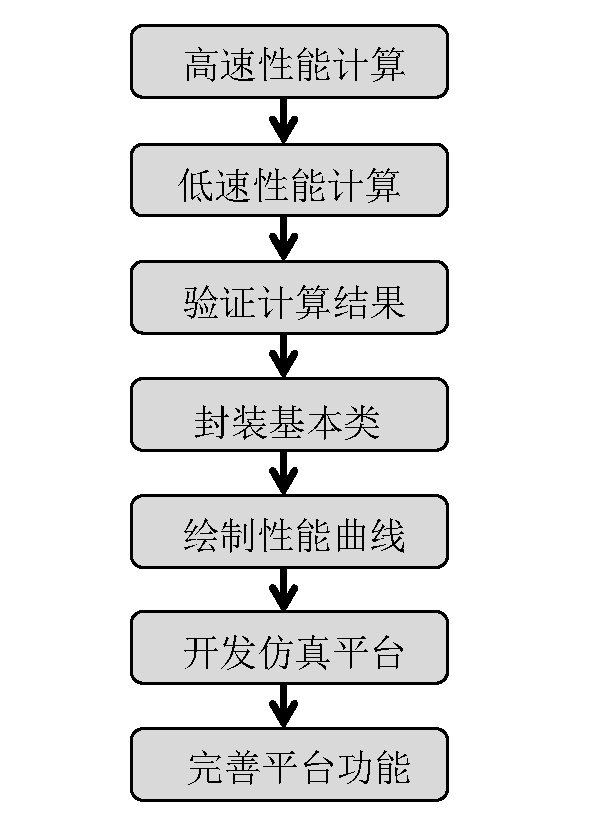
\includegraphics[width=0.32\textwidth]{pic/flow.pdf}\hspace{30pt}
\caption{研究流程图}\label{flowchart}
\end{figure}

\chapter{高速性能计算}\label{highspeedperformance}

\section{BADA模型简介}

由欧洲空管中心研究建立的BADA模型是评估航空器性能的一种基础模型\cite{BADA}。BADA(Base of Aircraft Data)模型包括一系列的基础机型参数文件,并在其提供的手册中给出了利用这些参数计算各项性能数据的公式。欧洲空管中心为提高空管工作的运行效率,收集了大量的基本数据,结合飞机制造厂商的手册,建立较为粗略的性能模型。根据使用者反馈的模型的使用情况和改进意见,逐步对BADA模型进行优化改进,发布新的BADA版本。这些基础机型参数文件包括OPF(Operations Performance File,运行性能文件)、APF(Airline Procedures File,航空公司程序文件)以及GPF(Global Parameter File,全局参数文件)。本章的高速性能计算使用的是BADA 3.7版本。

\section{BADA模型性能计算}\label{BADAModel}

按照BADA使用手册中给出的各项计算公式,整理高速性能计算模型,包括标准大气模型、航空器速度、航空器运行边界、航空器气动模型、油耗模型和航空器机动性能。

表\ref{commonparameters}给出了全文所有相关公式中所用常见变量的意义与单位。

\begin{table}[!ht]
	\caption{常见变量说明}\label{commonparameters}
	\begin{tabular*}{\hsize}{@{}@{\extracolsep{\fill}}lll@{}}
		\toprule[1.5pt]
		变量符号  &说明  &单位\\
		\midrule[0.5pt]
		$h$  &气压高度   &$\rm ft$\\
		$v_{\rm CAS}$  &校正空速  &$\rm m/s$\\
		$m$  &航空器实际重量 &$\rm kg$\\
		$\Delta \rm ISA$  &实际大气温度偏离标准大气(ISA)的值  &$\rm K(^\circ)$\\
		$\phi$  &坡度角  &$\rm degr$\\
		$e_{\rm index}$  &发动机种类(1:喷气发动机;2:涡桨发动机;3:活塞发动机)  &-\\
		\bottomrule[1.5pt]
	\end{tabular*}
\end{table}

\subsection{标准大气模型}

在标准大气模型中所用到的常量如表\ref{constantsInAtmosphereEnviroment}所示。

\begin{table}[!ht]
	\caption{标准大气模型常量说明}\label{constantsInAtmosphereEnviroment}
	\begin{tabular*}{\hsize}{@{}@{\extracolsep{\fill}}lll@{}}
		\toprule[1.5pt]
		常量符号  &说明  &数值\\
		\midrule[0.5pt]
		$P_{\rm 0}$  &标准大气海平面气压   &101325\ $\rm Pa$\\
		$T_{\rm 0}$  &标准大气海平面温度  &288.15\ $\rm K$\\
		$\rho_{\rm 0}$  &标准大气海平面空气密度 &1.225\ $\rm kg/m^3$\\
		$a_{\rm 0}$  &标准大气海平面音速  &340.29\ $\rm m/s$\\
		$g$  &重力加速度  &9.8\ $\rm m/s^2$\\
		$\gamma$  &空气等熵膨胀系数  &1.4\\
		$K_{\rm T}$  &标准大气温度垂直递减率(米)  &-0.0065 \ $\rm K(^\circ)/m$\\
		$K_{\rm T,ft}$  &标准大气温度垂直递减率(英尺) &-0.0019812 \ $\rm K(^\circ)/ft$\\
		$R$  &标准大气气体常数 &287.05287 \ $\rm m^2/(K\cdot s^2)$\\
		$\mu$  &空速转换中常量系数 &0.285714\\
		$T_{\rm trop}$  &标准大气对流层顶温度 &216.65\ $\rm K$\\
		$a_{\rm trop}$  &标准大气对流层顶音速 &295.07\ $\rm m/s$\\
		\bottomrule[1.5pt]
	\end{tabular*}
\end{table}

标准大气计算参数的方法如下。

(1)对流层顶高度$h_{\rm trop}$($\rm ft$):

\begin{equation}\label{htrop}
h_{\rm trop}=36089-\frac{\Delta \rm ISA}{K_{\rm T,ft}}
\end{equation}

其中$h_{\rm trop}$单位为$\rm ft$,$\Delta \rm ISA$为实际大气温度偏离标准大气(ISA)的值,单位为$\rm K(^\circ)$。

(2)大气温度$T$($\rm K$):

\begin{equation}
T=\left\{\begin{array}{ll}
T_{\rm 0}+h K_{\rm T,ft}   &   , h\textless h_{\rm trop},\\
T_{\rm trop}   &   , h\geq h_{\rm trop}
\end{array}\right.
\end{equation}

(3)大气压强$P$($\rm Pa$):

\begin{equation}
P=\left\{\begin{array}{ll}
P_{\rm 0}(\frac{T}{T_{\rm 0}})^{5.25583}   &   , h\textless h_{\rm trop},\\
e^{-\frac{g}{R T_{\rm trop}} \frac{h-h_{\rm trop}}{3.28}}P_{\rm trop}   &   , h\geq h_{\rm trop}
\end{array}\right.
\end{equation}

其中$P_{\rm trop}$为对流层顶大气压强,按下述公式计算:

\begin{equation}
P_{\rm trop}=P_{\rm 0}\left(\frac{T_{\rm trop}}{T_{\rm 0}}\right)^{5.25583}
\end{equation}

(4)大气密度$\rho$($\rm kg/m^3$):

\begin{equation}
\rho=\left\{\begin{array}{ll}
\rho_{\rm 0}(\frac{T}{T_{\rm 0}})^{4.25583}   &   , h\textless h_{\rm trop},\\
e^{-\frac{g}{R T_{\rm trop}} \frac{h-h_{\rm trop}}{3.28}}\rho_{\rm trop}   &   , h\geq h_{\rm trop}
\end{array}\right.
\end{equation}

其中$\rho_{\rm trop}$为对流层顶大气压强,按下述公式计算:

\begin{equation}
\rho_{\rm trop}=\rho_{\rm 0}\left(\frac{T_{\rm trop}}{T_{\rm 0}}\right)^{4.25583}
\end{equation}

(5)音速$a$($\rm m/s$):

\begin{equation}
a=\left\{\begin{array}{ll}
a_{\rm 0}\sqrt{\frac{T}{T_{\rm 0}}}   &   , h\textless h_{\rm trop},\\
a_{\rm trop}   &   , h\geq h_{\rm trop}
\end{array}\right.
\end{equation}

(6)真空速$v_{\rm TAS}$($\rm m/s$):

\begin{equation}\label{TAS}
v_{\rm TAS}=\sqrt{\frac{2}{\mu} \frac{P}{\rho} \left\{\left(1+\frac{P_{\rm 0}}{P}\left[(1+\frac{\mu}{2}\frac{\rho_{\rm 0}}{P_{\rm 0}}v_{\rm CAS}^2)^{\frac{1}{\mu}}-1\right]\right)^\mu -1\right\}}
\end{equation}

(7)校正空速$v_{\rm CAS}$($\rm m/s$):

\begin{equation}\label{CAS}
v_{\rm CAS}=\sqrt{\frac{2}{\mu} \frac{P_{\rm 0}}{\rho_{\rm 0}} \left\{\left(1+\frac{P}{P_{\rm 0}}\left[(1+\frac{\mu}{2}\frac{\rho}{P}v_{\rm TAS}^2)^{\frac{1}{\mu}}-1\right]\right)^\mu -1\right\}}
\end{equation}

(8)马赫数$M$:

\begin{equation}
M=\frac{v_{\rm TAS}}{a}
\end{equation}

(9)过渡高度$h_{\rm cross}$($\rm ft$):

\begin{equation}\label{hCross}
h_{\rm cross}=\frac{T_{\rm 0}(\theta_{\rm cross}-1)}{0.3048 K_{\rm T}}
\end{equation}

其中$\theta_{\rm cross}$由下两式确定:

\begin{equation}
\theta_{\rm cross}=\left(\delta_{\rm cross}\right)^{-\frac{K_{\rm T}R}{g}}
\end{equation}

\begin{equation}
\delta_{\rm cross}=\frac{\left[1+\frac{\gamma -1}{2} \left(\frac{v_{\rm CAS}}{a_{\rm 0}}\right)^2\right]^{\frac{\gamma}{\gamma -1}}-1}{\left[1+\frac{\gamma -1}{2} M^2\right]^{\frac{\gamma}{\gamma -1}}-1}
\end{equation}


\subsection{航空器速度}

(1)速度修正公式

\begin{equation}\label{VCorrection}
v_{\rm corrected}=v_{\rm ref}\times \sqrt{\frac{m}{m_{\rm ref}}}
\end{equation}

其中$v_{\rm corrected}$为修正重量后的速度,$v_{\rm ref}$为修正前的参考速度,两者单位一致。$m_{\rm ref}$在OPF文件中给出。


(2)爬升速度$v_{\rm climb}$($\rm kt$ CAS):

若$e_{\rm index}$为1,则

\begin{equation}
v_{\rm climb}=\left\{\begin{array}{ll}
C_{\rm V,min}\times v_{\rm stall,TO}+v_{\rm d,Cl,1}   &   , 0\leq h\leq 1499,\\
C_{\rm V,min}\times v_{\rm stall,TO}+v_{\rm d,Cl,2}   &   , 1500\leq h\leq 2999,\\
C_{\rm V,min}\times v_{\rm stall,TO}+v_{\rm d,Cl,3}   &   , 3000\leq h\leq 3999,\\
C_{\rm V,min}\times v_{\rm stall,TO}+v_{\rm d,Cl,4}   &   , 4000\leq h\leq 4999,\\
C_{\rm V,min}\times v_{\rm stall,TO}+v_{\rm d,Cl,5}   &   , 5000\leq h\leq 5999,\\
{\rm min}\left\{ v_{\rm Cl,1},250\right\}   &   , 6000\leq h\leq 10000,\\
v_{\rm Cl,2}   &   , 10000\textless h\leq h_{\rm cross},\\
M_{\rm Cl}   &   , h\textgreater h_{\rm cross}
\end{array}\right.
\end{equation}

若$e_{\rm index}$为2或3,则

\begin{equation}
v_{\rm climb}=\left\{\begin{array}{ll}
C_{\rm V,min}\times v_{\rm stall,TO}+v_{\rm d,Cl,6}   &   , 0\leq h\leq 499,\\
C_{\rm V,min}\times v_{\rm stall,TO}+v_{\rm d,Cl,7}   &   , 500\leq h\leq 999,\\
C_{\rm V,min}\times v_{\rm stall,TO}+v_{\rm d,Cl,8}   &   , 1000\leq h\leq 1499,\\
{\rm min}\left\{ v_{\rm Cl,1},250\right\}   &   , 1500\leq h\leq 9999,\\
v_{\rm Cl,2}   &   , 10000\leq h\leq h_{\rm cross},\\
M_{\rm Cl}   &   , h\textgreater h_{\rm cross}
\end{array}\right.
\end{equation}

其中$C_{\rm V,min}$、$v_{\rm stall,TO}$、$v_{\rm d,Cl,1}$至$v_{\rm d,Cl,8}$在GPF文件中给出,$v_{\rm Cl,1}$、$v_{\rm Cl,2}$及$M_{\rm Cl}$在APF文件中给出。$h_{\rm cross}$由$v_{\rm Cl,2}$和$M_{\rm Cl}$,根据式\ref{hCross}计算得到。需要注意的是,由于$v_{\rm climb}$为CAS,需要用$M_{\rm Cl}$得到TAS,再将TAS转化为CAS。另外,$v_{\rm stall,TO}$需根据航空器实际重量,按式\ref{VCorrection}进行修正。

(3)巡航速度$v_{\rm cruise}$($\rm kt$ CAS):

若$e_{\rm index}$为1,则

\begin{equation}
v_{\rm cruise}=\left\{\begin{array}{ll}
170   &   , 0\leq h\leq 2999,\\
{\rm min}\left\{ v_{\rm Cr,1},220\right\}   &   , 3000\leq h\leq 5999,\\
{\rm min}\left\{ v_{\rm Cr,1},250\right\}   &   , 6000\leq h\leq 13999,\\
v_{\rm Cr,2}   &   , 14000\textless h\leq h_{\rm cross},\\
M_{\rm Cr}   &   , h\textgreater h_{\rm cross}
\end{array}\right.
\end{equation}

若$e_{\rm index}$为2,则

\begin{equation}
v_{\rm cruise}=\left\{\begin{array}{ll}
150   &   , 0\leq h\leq 2999,\\
{\rm min}\left\{ v_{\rm Cr,1},180\right\}   &   , 3000\leq h\leq 5999,\\
{\rm min}\left\{ v_{\rm Cr,1},250\right\}   &   , 6000\leq h\leq 9999,\\
v_{\rm Cr,2}   &   , 10000\textless h\leq h_{\rm cross},\\
M_{\rm Cr}   &   , h\textgreater h_{\rm cross}
\end{array}\right.
\end{equation}

其中$v_{\rm Cr,1}$、$v_{\rm Cr,2}$及$M_{\rm Cr}$在APF文件中给出。$h_{\rm cross}$由$v_{\rm Cr,2}$和$M_{\rm Cr}$,根据式\ref{hCross}计算得到。

(4)下降速度$v_{\rm descent}$($\rm kt$ CAS):

若$e_{\rm index}$为1或2,则

\begin{equation}\label{vdescent1}
v_{\rm descent}=\left\{\begin{array}{ll}
C_{\rm V,min}\times v_{\rm stall,LD}+v_{\rm d,des,1}   &   , 0\leq h\leq 999,\\
C_{\rm V,min}\times v_{\rm stall,LD}+v_{\rm d,des,2}   &   , 1000\leq h\leq 1499,\\
C_{\rm V,min}\times v_{\rm stall,LD}+v_{\rm d,des,3}   &   , 1500\leq h\leq 1999,\\
C_{\rm V,min}\times v_{\rm stall,LD}+v_{\rm d,des,4}   &   , 2000\leq h\leq 2999,\\
{\rm min}\left\{ v_{\rm des,2},220\right\}   &   , 3000\leq h\leq 6000,\\
{\rm min}\left\{ v_{\rm des,2},250\right\}   &   , 6000\textless h\leq 10000,\\
v_{\rm des,1}   &   , 10000\textless h\leq h_{\rm cross},\\
M_{\rm des}   &   , h\textgreater h_{\rm cross}
\end{array}\right.
\end{equation}

若$e_{\rm index}$为3,则

\begin{equation}\label{vdescent2}
v_{\rm descent}=\left\{\begin{array}{ll}
C_{\rm V,min}\times v_{\rm stall,LD}+v_{\rm d,des,5}   &   , 0\leq h\leq 499,\\
C_{\rm V,min}\times v_{\rm stall,LD}+v_{\rm d,des,6}   &   , 500\leq h\leq 999,\\
C_{\rm V,min}\times v_{\rm stall,LD}+v_{\rm d,des,7}   &   , 1000\leq h\leq 1499,\\
v_{\rm des,2}   &   , 1500\leq h\leq 10000,\\
v_{\rm des,1}   &   , 10000\textless h\leq h_{\rm cross},\\
M_{\rm des}   &   , h\textgreater h_{\rm cross}
\end{array}\right.
\end{equation}

其中$v_{\rm stall,LD}$、$v_{\rm d,des,1}$至$v_{\rm d,des,7}$在GPF文件中给出,$v_{\rm des,1}$、$v_{\rm des,2}$及$M_{\rm des}$在APF文件中给出。$h_{\rm cross}$由$v_{\rm des,1}$和$M_{\rm des}$,根据式\ref{hCross}计算得到。同样地,为了计算以CAS表示的$v_{\rm des}$,需要用$M_{\rm des}$得到TAS,再将TAS转化为CAS。另外,$v_{\rm stall,LD}$需根据航空器实际重量,按式\ref{VCorrection}进行修正。

(4)等待速度$v_{\rm hold}$($\rm kt$ CAS):

\begin{equation}
v_{\rm hold}=\left\{\begin{array}{ll}
v_{\rm hold,1}   &   , 0\leq h\leq 14000,\\
v_{\rm hold,2}   &   , 14000\textless h\leq 20000,\\
v_{\rm hold,3}   &   , 20000\textless h\leq 34000,\\
M_{\rm hold}   &   , h\textgreater 34000
\end{array}\right.
\end{equation}

式中$v_{\rm hold,1}$至$v_{\rm hold,3}$及$M_{\rm hold}$在GPF文件中给出。同理,对$M_{\rm hold}$应先计算对应的TAS,再转化为CAS。


\subsection{航空器运行边界}

(1)实际最大飞行高度$h_{\rm max,actual}$($\rm ft$):

\begin{equation}\label{hmax,act}
h_{\rm max,actual}=\left\{\begin{array}{ll}
h_{\rm MO}, \text{仅当}h_{\rm max}=0\text{时},\\
{\rm min}\left\{ h_{\rm MO}, h_{\rm max}+G_t\times {\rm max}\left\{ 0, \Delta \rm ISA-C_{\rm T_{c,4}}\right\} +G_w\times \left(m_{\rm max}-m\right)\right\} 
\end{array}\right.
\end{equation}

其中,$h_{\rm max}$、$h_{\rm MO}$、$G_t$、$C_{\rm T_{c,4}}$、$G_w$、$m_{\rm max}$均在机型参数的OPF文件中给出。

(2)低速抖振马赫数$M_{\rm LBO}$

关于低速抖振马赫数的计算,BADA 3.7的使用手册给出了如下方程:

\begin{equation*}
k\times M^3-C_{\rm LBO,M=0}\times M^2+\frac{W}{0.583 S\cdot P}=0
\end{equation*}

式中的$k$为升力系数梯度,$C_{\rm LBO,M=0}$为$M=0$时初始抖振边界升力系数,$W$为航空器重($mg$),$S$为参考机翼面积,$P$为大气压强。解此方程中的$M$即可得到某一高度的低速抖振马赫数。然而,按手册附录提供的解一元三次方程方法,得到的低速抖振马赫数偏大。查阅后续版本的BADA手册发现,在解低速抖振方程时各版本所用公式存在冲突,故舍弃BADA模型中得到低速抖振边界的方法。

由于低速抖振马赫数和高速抖振马赫数为升力系数$C_{\rm L}$与马赫数$M$、最大升力系数$C_{\rm L,max}$与马赫数$M$这两条图线的左右交点处$M$的取值,故转而从图线交点获得低速抖振马赫数。

升力系数$C_{\rm L}$与马赫数间的关系如下所示:

\begin{equation}\label{CL-M}
C_{\rm L}=\frac{2mg}{\rho \left(M a\right)^2 S \cos\phi}
\end{equation}

由上式可以得到$C_{\rm L}$与$M$的曲线。$C_{\rm L,max}$与$M$之间的关系则非常复杂,很难使用公式描述两者之间的关系。考虑到各机型的$C_{\rm L,max}$差别较小,这里以波音737-800型飞机手册中提供的$C_{\rm L,max}$与$M$数据为基准,利用系数$factor$对$M$对应的$C_{\rm L,max}$进行修正,得到其他机型的$C_{\rm L,max}$\ -\ $M$曲线。在绘制完整曲线时,并未采取拟合得到函数式,使用线性插值得到了一条典型的$C_{\rm L,max}$与$M$曲线。将$C_{\rm L}$\ -\ $M$图线与之结合,两条曲线左交点对应的$M$即为低速抖振马赫数。

将各个高度上的低速抖振马赫数与对应机型性能图册的Buffet Limit Onset图线相比,发现结果符合较好。

(3)失速速度$v_{\rm stall}$($\rm kt$ CAS)

首先引入一个航空器飞行阶段的标识变量$FlightPhase$,这个变量将在后面的多个公式中使用。

\begin{equation*}
FlightPhase=\left\{\begin{array}{ll}
0   &   , \text{停机坪运行阶段},\\
1   &   , \text{滑行阶段},\\
2   &   , \text{起飞阶段},\\
3   &   , \text{爬升阶段},\\
4   &   , \text{巡航阶段},\\
5   &   , \text{下降阶段},\\
6   &   , \text{进近阶段},\\
7   &   , \text{着陆阶段},\\
8   &   , \text{执行等待阶段}
\end{array}\right.
\end{equation*}

失速速度$v_{\rm stall}$按如下方式确定:

\begin{equation}\label{vstall}
v_{\rm stall}=\left\{\begin{array}{ll}
v_{\rm stall,TO}   &   , 0\leq h\leq H_{\rm max,TO}\text{且}FlightPhase=2\text{或}3,\\                      
v_{\rm stall,IC}   &   , H_{\rm max,TO}\textless h\leq H_{\rm max,IC}\text{且}FlightPhase=3,\\  
v_{\rm stall,CR}   &   , h\textgreater H_{\rm max,IC}\text{且}FlightPhase=3,\\
				&   \ \ \text{或}h\textgreater H_{\rm max,AP}\text{且}FlightPhase=4\text{或}5,\\
				&   \ \ \text{或}h\textless H_{\rm max,AP}\text{且}FlightPhase=5\text{且}v_{\rm descent}\geq C_{\rm V,min}\times v_{\rm stall,CR}+10,\\
v_{\rm stall,AP}   &   , H_{\rm max,LD}\leq h\leq H_{\rm max,AP}\text{且}FlightPhase=5\\
  &   \ \ \ \ \ \ \ \ \ \ \ \ \ \ \ \ \ \ \ \ \ \ \ \ \ \ \ \ \ \ \ \ \ \ \ \ \ \ \ \ \ \ \text{且}v_{\rm descent}\textless C_{\rm V,min}\times v_{\rm stall,CR}+10,\\
  &   \ \ \text{或}h\textless H_{\rm max,LD}\text{且}FlightPhase=5\text{且}v_{\rm descent}\geq C_{\rm V,min}\times v_{\rm stall,AP}+10,\\
v_{\rm stall,LD}   &   , h\textless H_{\rm max,LD}\text{且}FlightPhase=5\text{且}v_{\rm descent}\textless C_{\rm V,min}\times v_{\rm stall,AP}+10
\end{array}\right.
\end{equation}

其中,$v_{\rm stall,TO}$、$v_{\rm stall,IC}$、$v_{\rm stall,CR}$、$v_{\rm stall,AP}$、$v_{\rm stall,LD}$以及$H_{\rm max,TO}$、$H_{\rm max,IC}$、$H_{\rm max,AP}$、$H_{\rm max,LD}$分别在OPF和GPF文件中给出。$v_{\rm descent}$由式\ref{vdescent1}或\ref{vdescent2}得到。

(4)飞行最低速度$v_{\rm min}$($\rm kt$ CAS)

$v_{\rm min}$是$C_{\rm V,min}$倍的失速速度$v_{\rm stall}$与低速抖振边界速度两者中较大的一个。$v_{\rm min}$按如下公式确定:

\begin{equation}
v_{\rm min}=\left\{\begin{array}{ll}
C_{\rm V,mim,TO}\times v_{\rm stall}   &   , 0\leq h\leq H_{\rm max,TO}\text{且}FlightPhase=2,\\                  
{\rm max}\left\{ C_{\rm V,mim}\times v_{\rm stall},v_{\rm CAS}\left(M_{\rm LBO}\times a\right)\right\}   &   , h\textgreater 15000\text{且}e_{\rm index}=1,\\
&   \ \ \text{或}h\textgreater 15000\text{且}C_{\rm LBO,M=0}\neq 0,\\
C_{\rm V,mim}\times v_{\rm stall}   &   , \text{其他}
\end{array}\right.
\end{equation}

其中,$C_{\rm V,mim,TO}$在GPF文件中给出。$v_{\rm stall}$由式\ref{vstall}得到。$v_{\rm CAS}()$的含义为括号中的数值为TAS,通过式\ref{CAS}换算为CAS。同理,下文中$v_{\rm TAS}()$的含义为将括号中的CAS数值根据式\ref{TAS}换算成TAS。


\subsection{航空器气动模型}\label{fM}

(1)升力系数$C_{\rm L}$

升力系数的公式由式\ref{CL-M}变形得到,如下所示。

\begin{equation}\label{CL}
C_{\rm L}=\frac{2mg}{\rho v_{\rm TAS}^2 S \cos\phi}
\end{equation}

(2)阻力系数$C_{\rm D}$

若OPF文件中的$C_{\rm D0,AP}$、$C_{\rm D2,AP}$、$C_{\rm D0,LDG}$、$C_{\rm D0,\Delta LDG}$及$C_{\rm D2,LDG}$均为0,则

\begin{equation}
C_{\rm D}=C_{\rm D0,Cr}+C_{\rm D2,Cr}C_{\rm L}^2
\end{equation}

若$C_{\rm D0,AP}$、$C_{\rm D2,AP}$、$C_{\rm D0,LDG}$、$C_{\rm D0,\Delta LDG}$及$C_{\rm D2,LDG}$均不为0,则

\begin{equation}\label{CDrag}
C_{\rm D}=\left\{\begin{array}{ll}
C_{\rm D0,AP}+C_{\rm D2,AP}C_{\rm L}^2   &   , FlightPhase=6,\\                  
C_{\rm D0,LDG}+C_{\rm D0,\Delta LDG}+C_{\rm D2,LDG}C_{\rm L}^2   &   , FlightPhase=7,\\     
C_{\rm D0,Cr}+C_{\rm D2,Cr}C_{\rm L}^2   &   , \text{其他}
\end{array}\right.
\end{equation}

其中,$C_{\rm D0,AP}$、$C_{\rm D2,AP}$、$C_{\rm D0,Cr}$、$C_{\rm D2,Cr}$均在OPF文件中给出。

(3)阻力$D$($\rm N$):

\begin{equation}\label{Drag}
D=\frac{C_{\rm D}\rho v_{\rm TAS}^2 S}{2}
\end{equation}

(4)加速下降阻力$D_{\rm des,expedite}$($\rm N$)

在下降阶段,有时航空器需要加速下降从而在规定时间内完成高高度下降。此时的阻力

\begin{equation}\label{Dexp}
D_{\rm des,expedite}=C_{\rm des,exp}\times D
\end{equation}

其中$D$由式\ref{Drag}得到,$C_{\rm des,exp}$在GPF文件中给出。

(5)最大爬升推力$T_{\rm max,climb}$($\rm N$)

最大爬升推力为航空器爬升阶段使用的最大推力。值得注意的是$T_{\rm max,climb}$并非TOGA推力,根据计算结果与性能手册中TOGA推力的大小比对,发现TOGA推力大约为$T_{\rm max,climb}$的1.1倍。$T_{\rm max,climb}$按下列式子确定:

\begin{equation}
T_{\rm max,climb,standard}=\left\{\begin{array}{ll}
C_{\rm T_{\rm C,1}}\times\left(1-\frac{h}{C_{\rm T_{\rm C,2}}}+C_{\rm T_{\rm C,3}}\times h^2\right)   &   , e_{\rm index}=1,\\        
&\\          
\frac{C_{\rm T_{\rm C,1}}\times \left(1-\frac{h}{C_{\rm T_{\rm C,2}}}\right)}{v_{\rm TAS}}+C_{\rm T_{\rm C,3}}   &   , e_{\rm index}=2,\\     
&\\
C_{\rm T_{\rm C,1}}\times\left(1-\frac{h}{C_{\rm T_{\rm C,2}}}\right)+\frac{C_{\rm T_{\rm C,3}}}{v_{\rm TAS}}   &   , e_{\rm index}=3
\end{array}\right.
\end{equation}

上式为标准大气环境下的最大爬升推力,加入修正项系数$C_{\left(\Delta \rm ISA\right)_{\rm eff}}$:

令

\begin{equation}
\left(\Delta \rm ISA\right)_{\rm eff}=\Delta \rm ISA-C_{\rm T_{\rm C,4}}
\end{equation}

若$\left(\Delta \rm ISA\right)_{\rm eff}$满足

\begin{equation}
0\leq\left(\Delta \rm ISA\right)_{\rm eff}\times C_{\rm T_{\rm C,5}}\leq 0.4
\end{equation}

则

\begin{equation}
C_{\left(\Delta \rm ISA\right)_{\rm eff}}=1-\left(\Delta \rm ISA\right)_{\rm eff}\times C_{\rm T_{\rm C,5}}
\end{equation}

最终得到的最大爬升推力为

\begin{equation}
T_{\rm max,climb}=C_{\left(\Delta \rm ISA\right)_{\rm eff}}\times T_{\rm max,climb,standard}
\end{equation}

上述式子中,$C_{\rm T_{\rm C,1}}$至$C_{\rm T_{\rm C,5}}$均在OPF文件中给出。

(6)巡航推力$T_{\rm cruise}$($\rm N$)

正常巡航推力等于巡航中航空器所受阻力,即

\begin{equation}
T_{\rm cruise}=D
\end{equation}

式中$D$为巡航阶段所受阻力,由式\ref{Drag}确定。

(7)最大巡航推力$T_{\rm max,cruise}$($\rm N$)

最大巡航推力为正常巡航推力的$C_{\rm T,Cr}$倍。$C_{\rm T,Cr}$在GPF文件中给出。

\begin{equation}
T_{\rm max,cruise}=C_{\rm T,Cr}\times T_{\rm cruise}
\end{equation}

(8)下降推力$T_{\rm des}$($\rm N$)

在高空,即$h\textgreater h_{\rm des}$且$FlightPhase=5$时,

\begin{equation}
T_{\rm des}=C_{\rm des,high}\times T_{\rm max,climb}
\end{equation}

在低空,即$h\leq h_{\rm des}$时,有

\begin{equation}
T_{\rm des}=\left\{\begin{array}{ll}
T_{\rm des}=C_{\rm des,low}\times T_{\rm max,climb}   &   , FlightPhase=5,\\        
T_{\rm des}=C_{\rm des,app}\times T_{\rm max,climb}   &   , FlightPhase=6,\\     
T_{\rm des}=C_{\rm des,ld}\times T_{\rm max,climb}   &   , FlightPhase=7
\end{array}\right.
\end{equation}

上两式中,$h_{\rm des}$、$C_{\rm des,high}$、$C_{\rm des,low}$、$C_{\rm des,app}$、$C_{\rm des,ld}$均在OPF文件中给出。

(9)推力$T$($\rm N$)

综合上述有关推力的公式,推力

\begin{equation}
T=\left\{\begin{array}{ll}
T_{\rm max,climb}   &   , FlightPhase=3,\\        
T_{\rm cruise}   &   , FlightPhase=4\text{且使用正常巡航推力},\\   
T_{\rm max,cruise}   &   , FlightPhase=4\text{且使用最大巡航推力},\\   
T_{\rm des}   &   , FlightPhase=5\text{或}6\text{或}7
\end{array}\right.
\end{equation}


(10)减推力系数$C_{\rm power,reduce}$

减推力爬升是航空器常用的爬升方式。减推力系数为最大爬升推力的折减系数,在未修正航空器实际重量时

\begin{equation}
C_{\rm power,reduce,standard}=\left\{\begin{array}{ll}
C_{\rm reduce,jet}   &   , e_{\rm index}=1,\\        
C_{\rm reduce,turbo}   &   , e_{\rm index}=2,\\     
C_{\rm reduce,piston}   &   , e_{\rm index}=3
\end{array}\right.
\end{equation}

其中$C_{\rm reduce,jet}$、$C_{\rm reduce,turbo}$和$C_{\rm reduce,piston}$在GPF文件中给出。

按航空器重量修正,

\begin{equation}
C_{\rm power,reduce}=1-C_{\rm power,reduce,standard}\frac{m_{\rm max}-m}{m_{\rm max}-m_{\rm min}}
\end{equation}

式中$m_{\rm max}$与$m_{\rm min}$在OPF文件中给出。

(11)能量转移因子(加速因子)$f\{M\}$

在爬升/下降率的计算中,能量转移因子(即加速因子)的表达式为

\begin{equation}
f\{M\}=\left[1+\frac{v_{\rm TAS}}{g}\frac{{\rm d}v_{\rm TAS}}{{\rm d}h}\right]^{-1}
\end{equation}

为简便计算,BADA模型提供了能量转移因子的另一种计算方法。首先引入航空器运动姿态的标识变量$AttitudeAndMovement$:

\begin{equation}
AttitudeAndMovement=\left\{\begin{array}{ll}
0   &   , \text{定常飞行},\\        
1   &   , \text{爬升加速},\\     
2   &   , \text{爬升减速},\\     
3   &   , \text{下降加速},\\     
4   &   , \text{下降减速}
\end{array}\right.
\end{equation}

当$AttitudeAndMovement\neq 0$时,$f\{M\}$有固定取值:

\begin{equation}
f\{M\}=\left\{\begin{array}{ll}
0.3   &   , AttitudeAndMovement=1\text{或}3,\\        
1.7   &   , AttitudeAndMovement=2\text{或}4
\end{array}\right.
\end{equation}

当$AttitudeAndMovement=0$即航空器处于定常飞行状态时,$f\{M\}$的计算区分两种飞行模式:

若航空器按等马赫数飞行,则有

\begin{equation}
f\{M\}=\left\{\begin{array}{ll}
\left(1+\frac{\gamma RK_{\rm T}}{2g}M^2\right)^{-1}   &   , 0\leq h\leq h_{\rm trop},\\        
1   &   , h\textgreater h_{\rm trop}
\end{array}\right.
\end{equation}

式中$M$为所保持的马赫数。

若航空器按等校正空速飞行,则有

\begin{equation}
M=\frac{v_{\rm TAS}\left(v_{\rm CAS}\right)}{a}
\end{equation}

式中$v_{\rm CAS}$为所保持的校正空速,

\begin{equation}
f\{M\}=\left\{\begin{array}{ll}
\left\{{1+\left(1+\frac{\gamma -1}{2}M^2\right)^{-\frac{1}{\gamma -1}}\left[\left(1+\frac{\gamma -1}{2}M^2\right)^{\frac{\gamma}{\gamma -1}}-1\right]+\frac{\gamma RK_{\rm T}}{2g}M^2}\right\}^{-1}   &   , 0\leq h\leq h_{\rm trop},\\       
\left\{{1+\left(1+\frac{\gamma -1}{2}M^2\right)^{-\frac{1}{\gamma -1}}\left[\left(1+\frac{\gamma -1}{2}M^2\right)^{\frac{\gamma}{\gamma -1}}-1\right]}\right\}^{-1}   &   , h\textgreater h_{\rm trop}
\end{array}\right.
\end{equation}

其中$h_{\rm trop}$由式\ref{htrop}确定。常量$\gamma$、$R$、$K_{\rm T}$数值见表\ref{constantsInAtmosphereEnviroment}。

(12)爬升/下降率$ROCD$($\rm ft/min$)

根据下降率计算公式

\begin{equation*}
ROCD=\frac{{\rm d}h}{{\rm d}t}=\left[\frac{\left(T-D\right)v_{\rm TAS}}{mg}\right]f\left\{M\right\}
\end{equation*}

阻力$D$按航空器的下降状态,若为加速下降,$D$按式\ref{Dexp}计算,否则按式\ref{Drag}计算。

爬升/下降率

\begin{equation}
ROCD=\left\{\begin{array}{ll}
\left[\frac{\left(T-D\right)v_{\rm TAS}}{mg}\right]f\left\{M\right\}\cdot C_{\rm power,reduce}   &   , h\textless 0.8h_{\rm max,actual}\text{且}FlightPhase=3\\    
  &   \ \ \text{且使用减推力爬升},\\
\left[\frac{\left(T-D\right)v_{\rm TAS}}{mg}\right]f\left\{M\right\}   &   , \text{其他}
\end{array}\right.
\end{equation}

式中$h_{\rm max,actual}$由式\ref{hmax,act}确定。


\subsection{油耗模型}

燃油流量$ff$($\rm kg/min$)的计算方法如下。

若$e_{\rm index}$为1或2:

\begin{equation}
ff=\left\{\begin{array}{ll}
C_{\rm f3}\times\left(1-\frac{h}{C_{\rm f4}}\right)   &   , FlightPhase=5\text{且使用IDLE推力},\\    
\eta C_{\rm f,cr}T   &   , FlightPhase=4,\\
\eta T   &   , \text{其他}
\end{array}\right.
\end{equation}

式中$\eta$为燃油消耗率($\rm kg/(min\cdot kN)$),由下式确定:

\begin{equation}
\eta=\left\{\begin{array}{ll}
C_{\rm f1}\left(1+\frac{v_{\rm TAS}}{C_{\rm f2}}\right)   &   , e_{\rm index}=1,\\    
&\\
C_{\rm f1}\left(1-\frac{v_{\rm TAS}}{C_{\rm f2}}\right)\frac{v_{\rm TAS}}{1000}   &   , e_{\rm index}=2,
\end{array}\right.
\end{equation}

若$e_{\rm index}$为3:

\begin{equation}
ff=\left\{\begin{array}{ll}
C_{\rm f3}   &   , FlightPhase=5,\\    
C_{\rm f1}C_{\rm f,cr}   &   , FlightPhase=4,\\
C_{\rm f1}   &   , \text{其他}
\end{array}\right.
\end{equation}

上述式子中,$C_{\rm f1}$、$C_{\rm f2}$、$C_{\rm f3}$、$C_{\rm f4}$及$C_{\rm f,cr}$均在OPF文件中给出。



\subsection{航空器机动性能}

BADA模型同时给出了如下所示的航空器做机动动作的运行限制和相关参数计算方法。

(1)最大加速度限制

在GPF文件中给出了民航客机的最大水平加速度$a_{\rm l,max}$和最大垂直加速度$a_{\rm n,max}$。BADA模型规定,航空器在做机动动作时必须满足

\begin{equation}
\left|v_t-v_{t-1}\right|\leq a_{\rm l,max}\Delta t
\end{equation}

及

\begin{equation}
\left|\gamma_t-\gamma_{t-1}\right|\leq \frac{a_{\rm n,max}\Delta t}{v_{\rm TAS}}
\end{equation}

其中$t$与$t-1$分别标志做机动动作和机动动作之前的状态,$\Delta t$为$t-1$到$t$所经过的时间,$\gamma$为爬升/下降角,按下式计算:

\begin{equation}
\gamma=\sin^{-1}\left(\frac{h}{v_{\rm TAS}}\right)
\end{equation}

(2)转弯率$\varphi$($\rm ^\circ/s$):

\begin{equation}
\varphi=\frac{g}{v_{\rm TAS}}\tan\phi
\end{equation}

BADA模型在GPF文件中给出了航空器在各阶段的标称及最大允许转弯坡度角$\phi$,单位均为$\rm degr$。

(3)转弯半径$R_{\rm turning}$($\rm m$):

\begin{equation}
R_{\rm turning}=\frac{v_{\rm TAS}^2}{g\tan\phi}
\end{equation}



\section{BADA性能计算编程}

使用\ref{BADAModel}节中的公式与计算方法,编写AtmosphereEnviroment类与Aircraft类,分别计算大气模型与航空器性能模型中的各项参数。按表\ref{commonparameters}中的公共参数,编写程序函数间的接口变量。除此之外,$FlightPhase$、$AttitudeAndMovement$等标识变量也作为接口,以枚举变量形式写入函数,方便用户调用。

为验证高速性能计算的准确性,编写代码读取空客300-600机型的BADA基本参数,包括其OPF、APF及GPF文件,创建Aircraft类,调用编写的函数计算性能数据。与BADA 3.7的使用手册中提供的该机型的PTF(Performance Tables Files,性能表格文件)比对后,函数的计算结果与其吻合较好,由此验证了根据BADA模型编写代码计算高速性能参数的正确性。

编写的函数中涉及多项默认参数、接口参数与函数输出值的物理单位转换,在主程序调用时务必注意阅读函数说明。为方便单位转换,编写了Units类供使用者调用。





\chapter{低速性能计算}\label{lowspeedperformance}

\section{飞机设计性能简介}

由于BADA模型提供的性能计算并不包含低速阶段,故采用《Civil Jet Aircraft Design》一书中低速性能的研究方法\cite{AircraftDesign},对航空器在起飞、着陆阶段时的性能建立运动模型、计算性能数据。书中的低速性能研究方法在航空器设计阶段使用,模型的建立较为粗糙。然而,书中的性能计算模型和现实情况相差很小,模型中的某些关键参数取值也是通过查阅大量机型性能手册统计得到。从开发仿真平台的角度来说,所得结果的准确性是可以接受的。

\section{飞机设计低速性能计算}

根据书中的飞机低速运动模型,整理得到了有关起飞距离、平衡场长、着陆距离的计算方法。


\subsection{起飞距离计算}\label{TOdistance}

起飞距离包括地面滑跑距离$s_{\rm ground}$和姿态转变距离$s_{\rm transition}$。两者及最终的起飞距离单位均为$\rm m$。

地面滑跑距离$s_{\rm ground}$计算方法如下。

\begin{equation}
K_{\rm T}=\frac{T}{W}-\mu
\end{equation}

其中$T$为所有发动机在TOGA状态的总推力,为

\begin{equation}
T=N\times 1.1T_{\rm max,climb}
\end{equation}

式中$N$为发动机数量。$W$为航空器重$mg$,$\mu$为跑道道面摩擦系数,具体取值为

\begin{equation}\label{mu}
\mu=\left\{\begin{array}{ll}
0.02   &   , \text{铺筑道面},\\    
0.04   &   , \text{硬石道面},\\
0.05   &   , \text{覆盖短草道面},\\
0.1   &   , \text{覆盖长草道面},\\
0.2   &   , \text{其他道面}
\end{array}\right.
\end{equation}

\begin{equation}\label{KA}
K_{\rm A}=\rho(\mu C_{\rm L}-C_{\rm D})\left(\frac{2W}{S}\right)^{-1}
\end{equation}

其中$C_{\rm L}$为起飞时升力系数,$C_{\rm D}$按式\ref{CDrag}中$FlightPhase=2$计算,$S$为飞机参考机翼面积。

模型给出飞机离地速度$v_{\rm LOF}$:

\begin{equation}
v_{\rm LOF}=1.1v_{\rm stall,TO}
\end{equation}

利用以上参数,得到飞机起飞地面滑跑距离

\begin{equation}
s_{\rm ground}=\frac{1}{2gK_{\rm A}}\ln\left(\frac{K_{\rm T}+K_{\rm A}v_{\rm LOF}^2}{K_{\rm T}}\right)
\end{equation}

飞机从离地到完成姿态转变为爬升的距离为$s_{\rm transition}$。首先取安全离地速度$v_{\rm 2}$:

\begin{equation}
v_{\rm 2}=1.2v_{\rm stall,TO}
\end{equation}

令姿态转变过渡速度$v_{\rm trans}$:

\begin{equation}
v_{\rm trans}=\frac{v_{\rm LOF}+v_{\rm 2}}{2}
\end{equation}

则飞机姿态转变时所飞圆弧的半径为

\begin{equation}
r=\frac{v_{\rm trans}^2}{g\left(n-1\right)}
\end{equation}

式中$n$为过载系数,取值为1.2。

飞机在起飞中的爬升梯度$\gamma$为

\begin{equation}
\gamma=\frac{T-D}{W}
\end{equation}

其中$D$按式\ref{Drag},令其中$v=v_{\rm 2}$得到。

起飞姿态转变距离为

\begin{equation}
s_{\rm transition,tem}=r\times\gamma
\end{equation}

飞机在跑道末端的高度必须不低于帘高$h_{\rm screen}$(screen height,一般为35\ $\rm ft$)。由此考察飞机在完成爬升姿态转变时到达的高度,若此时已高于帘高,可以缩短姿态转变距离;若低于帘高,则需要加长。

飞机在完成爬升姿态转变时到达的高度$h_{\rm trans}$为

\begin{equation}
h_{\rm trans}=\frac{r\theta^2}{2}
\end{equation}

式中$\theta$为飞行航迹角,由于角度较小,有$\theta\approx\gamma$。

将$h_{\rm trans}$与$h_{\rm screen}$进行大小比较,对$s_{\rm transition}$作出修正:

\begin{equation}
s_{\rm transition}=\left\{\begin{array}{ll}
s_{\rm transition,tem}+\frac{h_{\rm screen}-h_{\rm trans}}{\tan\gamma_{\rm c}}   &   , h_{\rm trans}\textless h_{\rm screen},\\   
&\\ 
\sqrt{\left(r+h_{\rm screen}\right)^2-r^2}   &   , h_{\rm trans}\geq h_{\rm screen}
\end{array}\right.
\end{equation}

其中$\gamma_{\rm c}$为最佳爬升角,由于角度很小,有$\tan\gamma_{\rm c}\approx\gamma$。

综合上述两段距离,得到最终的起飞距离为两段距离之和,加上15\%的余量:

\begin{equation}
s_{\rm TO}=\left(s_{\rm ground}+s_{\rm transition}\right)\times 1.15
\end{equation}



\subsection{平衡场长计算}

平衡场长的计算分为两部分,加速继续起飞和中断起飞起飞距离计算。加速继续起飞指航空器在决断速度$v_{\rm 1}$后遭遇发动机失效只能选择起飞所需起飞距离。中断起飞距离指在$v_{\rm 1}$前出现发动机失效,选择中断起飞所需跑道长度。

首先计算飞机在准备起飞到速度达到$v_{\rm 1}$前的地面滑跑距离$s_{\rm ground}$,这里$s_{\rm ground}$与\ref{TOdistance}节中所用方法一致,则有

\begin{equation}
s_{\rm ground}=\frac{1}{2gK_{\rm A}}\ln\left(\frac{K_{\rm T}+K_{\rm A}v_{\rm 1}^2}{K_{\rm T}}\right)
\end{equation}

在发动机失效时,假定飞行员需要2秒作出反应,则飞机将以$v_{\rm 1}$速度运动2秒,距离为

\begin{equation}
s_{\rm reaction}=2\times v_{\rm 1}
\end{equation}

(1)加速继续起飞距离$s_{\rm accelerate-go}$($\rm m$):

加速继续起飞距离的计算方法和\ref{TOdistance}节中类似,具体计算公式如下。

飞机在加速继续起飞起飞时,从$v_{\rm 1}$到$v_{\rm LOF}$所经过的距离$\Delta s$为:

在这段飞机的平均速度$v_{\rm m}$

\begin{equation}\label{v_m}
v_{\rm m}=\frac{v_{\rm 1}+v_{\rm LOF}}{2}
\end{equation}

计算$K_{\rm T}$:

\begin{equation}\label{KT1}
K_{\rm T}=\frac{T}{W}-\mu
\end{equation}

其中$T$为单发失效后发动机TOGA总推力,即

\begin{equation}\label{enginefailureT}
T=\left(N-1\right)\times 1.1T_{\rm max,climb}
\end{equation}

按式\ref{KA}计算$K_{\rm A}$,其中$C_{\rm L}$仍为起飞时升力系数,$C_{\rm D}$则除了式\ref{CDrag}所得到的阻力系数,还需加上两种附加阻力系数,即

\begin{equation}\label{enginefailureCD}
C_{\rm D}=C_{\rm D0,Cr}+C_{\rm D2,Cr}C_{\rm L}^2+C_{\rm D,windmilling}+C_{\rm D,asymmetric}
\end{equation}

$C_{\rm D,windmilling}$和$C_{\rm D,asymmetric}$为风车阻力系数和偏航阻力系数,取值分别为0.003486和0.00125。

根据式\ref{KT1}、\ref{KA}及\ref{v_m},可得加速度为

\begin{equation}\label{acceleration}
a=\frac{{\rm d}v}{{\rm d}t}=\left(K_{\rm T}+K_{\rm A}v_{\rm m}^2\right)g
\end{equation}

飞机在这一段所经过的时间$\Delta t$为

\begin{equation}
\Delta t=\frac{v_{\rm LOF}-v_{\rm 1}}{a}
\end{equation}

根据匀加速直线运动公式,得到飞机从$v_{\rm 1}$加速至$v_{\rm LOF}$所经过距离

\begin{equation}
\Delta s=v_{\rm 1}\Delta t+\frac{1}{2}a\left(\Delta t\right)^2
\end{equation}

之后计算飞机从$v_{\rm LOF}$到完成爬升姿态转变的距离,计算方法与\ref{TOdistance}节中相同。

\begin{equation}
v_{\rm m}=\frac{v_{\rm LOF}+v_{\rm 2}}{2}
\end{equation}

\begin{equation}
r=\frac{v_{\rm m}^2}{g\left(n-1\right)}
\end{equation}

\begin{equation}
\gamma=\frac{T-D}{W}
\end{equation}

注意式中$T$应使用式\ref{enginefailureT}得到,以及计算$D$时所用的阻力系数$C_{\rm D}$应使用式\ref{enginefailureCD}。

\begin{equation}
s_{\rm transition,tem}=r\times\gamma
\end{equation}

判断完成姿态转变时达到的高度与帘高大小关系,修正姿态转变距离:

\begin{equation}
h_{\rm trans}=\frac{r\theta^2}{2}
\end{equation}

\begin{equation}
s_{\rm transition}=\left\{\begin{array}{ll}
s_{\rm transition,tem}+\frac{h_{\rm screen}-h_{\rm trans}}{\tan\gamma_{\rm c}}   &   , h_{\rm trans}\textless h_{\rm screen},\\   
&\\ 
\sqrt{\left(r+h_{\rm screen}\right)^2-r^2}   &   , h_{\rm trans}\geq h_{\rm screen}
\end{array}\right.
\end{equation}

其中$\theta\approx\gamma\approx\tan\gamma_{\rm c}$。

则加速继续起飞距离为上述距离之和,再加上5\%的余量

\begin{equation}
s_{\rm accelerate-go}=\left(s_{\rm ground}+s_{\rm reaction}+\Delta s+s_{\rm transition}\right)\times 1.05
\end{equation}

(2)中断起飞距离$s_{\rm accelerate-stop}$($\rm m$):

对于发动机失效后中断起飞的距离,只需计算飞机从$v_{\rm 1}$减速至0所经过的距离。

在计算中断起飞距离时,跑道道面摩擦系数$\mu$并非由式\ref{mu}确定,而是取减速滑跑的道面摩擦系数,中断起飞情况下取0.3。又因为减速滑跑时推力$T$及升力系数$C_{\rm L}$均为0,故

\begin{equation}\label{KTwithoutT}
K_{\rm T}=\frac{T}{W}-\mu=-\mu
\end{equation}

\begin{equation}\label{KAwithoutCL}
K_{\rm A}=\rho(\mu C_{\rm L}-C_{\rm D})\left(\frac{2W}{S}\right)^{-1}=-\rho C_{\rm D}\left(\frac{2W}{S}\right)^{-1}
\end{equation}

其中$C_{\rm D}$按式\ref{CDrag}中$FlightPhase=7$计算。

由式\ref{acceleration}计算加速度$a$,其中平均速度

\begin{equation}
v_{\rm m}=\frac{v_{\rm 1}}{2}
\end{equation}

则根据匀减速直线运动公式,飞机从$v_{\rm 1}$直至停下所经过的距离为

\begin{equation}
s_{\rm stop}=-\frac{v_{\rm 1}^2}{2a}
\end{equation}

将上述距离相加,得到中断起飞距离

\begin{equation}
s_{\rm accelerate-stop}=s_{\rm ground}+s_{\rm reaction}+s_{\rm stop}
\end{equation}



\subsection{着陆距离计算}

书中对着陆距离的计算分为四个阶段:进近、改平、自由滑跑和减速停止阶段。

进近速度、着陆速度规定如下:

\begin{equation}
v_{\rm A}=1.3v_{\rm stall,LD}
\end{equation}

\begin{equation}
v_{\rm TD}=1.15v_{\rm stall,LD}
\end{equation}

改平阶段速度$v_{\rm F}$

\begin{equation}
v_{\rm F}=\frac{v_{\rm TD}+v_{\rm A}}{2}
\end{equation}

则改平阶段飞机经过的圆弧半径为

\begin{equation}
r=\frac{v_{\rm F}^2}{\left(n-1\right)g}
\end{equation}

其中$n$为过载系数,取1.2。

飞机在改平阶段高度

\begin{equation}
h_{\rm F}=\frac{r\gamma^2}{2}
\end{equation}

式中$\gamma$为最佳下降角,值为3\ $degr$,即0.0254 $\rm rad$。

则飞机在进近阶段经过距离$s_{\rm A}$及改平阶段距离$s_{\rm F}$分别为

\begin{equation}
s_{\rm A}=\frac{h_{\rm screen}-h_{\rm F}}{\gamma}
\end{equation}

\begin{equation}
s_{\rm F}=r\times \gamma
\end{equation}

其中$h_{\rm screen}$为帘高,一般为35\ $\rm ft$。

飞机在改平接地后有一段自由滑跑,假定时间为2秒,则自由滑跑段距离为

\begin{equation}
s_{\rm FR}=2\times v_{\rm TD}
\end{equation}

最后计算飞机着陆后的减速停止距离。飞机在着陆时的情形和中断起飞时相似,按式\ref{KTwithoutT}和\ref{KAwithoutCL}计算$K_{\rm T}$和$K_{\rm A}$,其中跑道道面摩擦系数$\mu$有下列取值:

\begin{equation}
\mu=\left\{\begin{array}{ll}
0.33   &   , \text{干跑道},\\    
0.1   &   , \text{湿跑道},\\
0.05   &   , \text{其他道面情况}
\end{array}\right.
\end{equation}

则飞机减速停止距离$s_{\rm B}$为

\begin{equation}
s_{\rm B}=-\frac{1}{2gK_{\rm A}}\ln\left(\frac{K_{\rm T}+K_{\rm A}v_{\rm TD}^2}{K_{\rm T}}\right)
\end{equation}

上式右端加入负号是因为加速度为负值,所得出的距离为负数,故需取相反数得到正值。

将以上距离相加的结果再加上66\%的余量,则得到最终的着陆距离$s_{\rm LD}$为

\begin{equation}
s_{\rm LD}=\left(s_{\rm A}+s_{\rm F}+s_{\rm FR}+s_{\rm B}\right)\times 1.66
\end{equation}



\section{低速性能计算编程}

对上一节所述计算起飞距离、平衡场长和着陆距离的公式在Aircraft类中编写代码。由于在同一个类中编写,需要把本章的输入参数接口和BADA模型所用参数衔接起来,保证在调用时使用表\ref{commonparameters}中的公共参数。

因为本章所用《Civil Jet Aircraft Design》一书编写时间距今已很久远,其中所述的低速性能研究方法只在飞机设计阶段使用,在编程计算时存在很多所得结果与现实情况的矛盾。通过查阅最新的性能手册,修正书中明显的公式错误,逐步调试模型中的常量参数,最终使得到的结果较为合理。

程序利用BADA 3.7给出的空客300-600型飞机的基本数据,计算该飞机的起飞距离和着陆距离,得到起飞所需距离为2361.77\ $\rm m$,着陆所需距离为1555.65\ $\rm m$。查询BADA 3.7空客300-600的OPF文件,其中给出了标称起飞距离为2362\ $\rm m$,着陆距离为1555\ $\rm m$。说明采用本章列出的低速性能计算方法得到的起飞、着陆距离与正确结果吻合较好。

程序绘制了如图\ref{verifybfl}所示的空客300-600机型的平衡场长,得到在加速继续起飞和中断起飞两条曲线交点处,该机型的平衡场长为2395.05\ $\rm m$,对应的决断速度$v_{\rm 1}$为127.01 $\rm kt$。所得结果及平衡场长中曲线的趋势均与现实情况符合较好。

\begin{figure}[h]
	\centering
	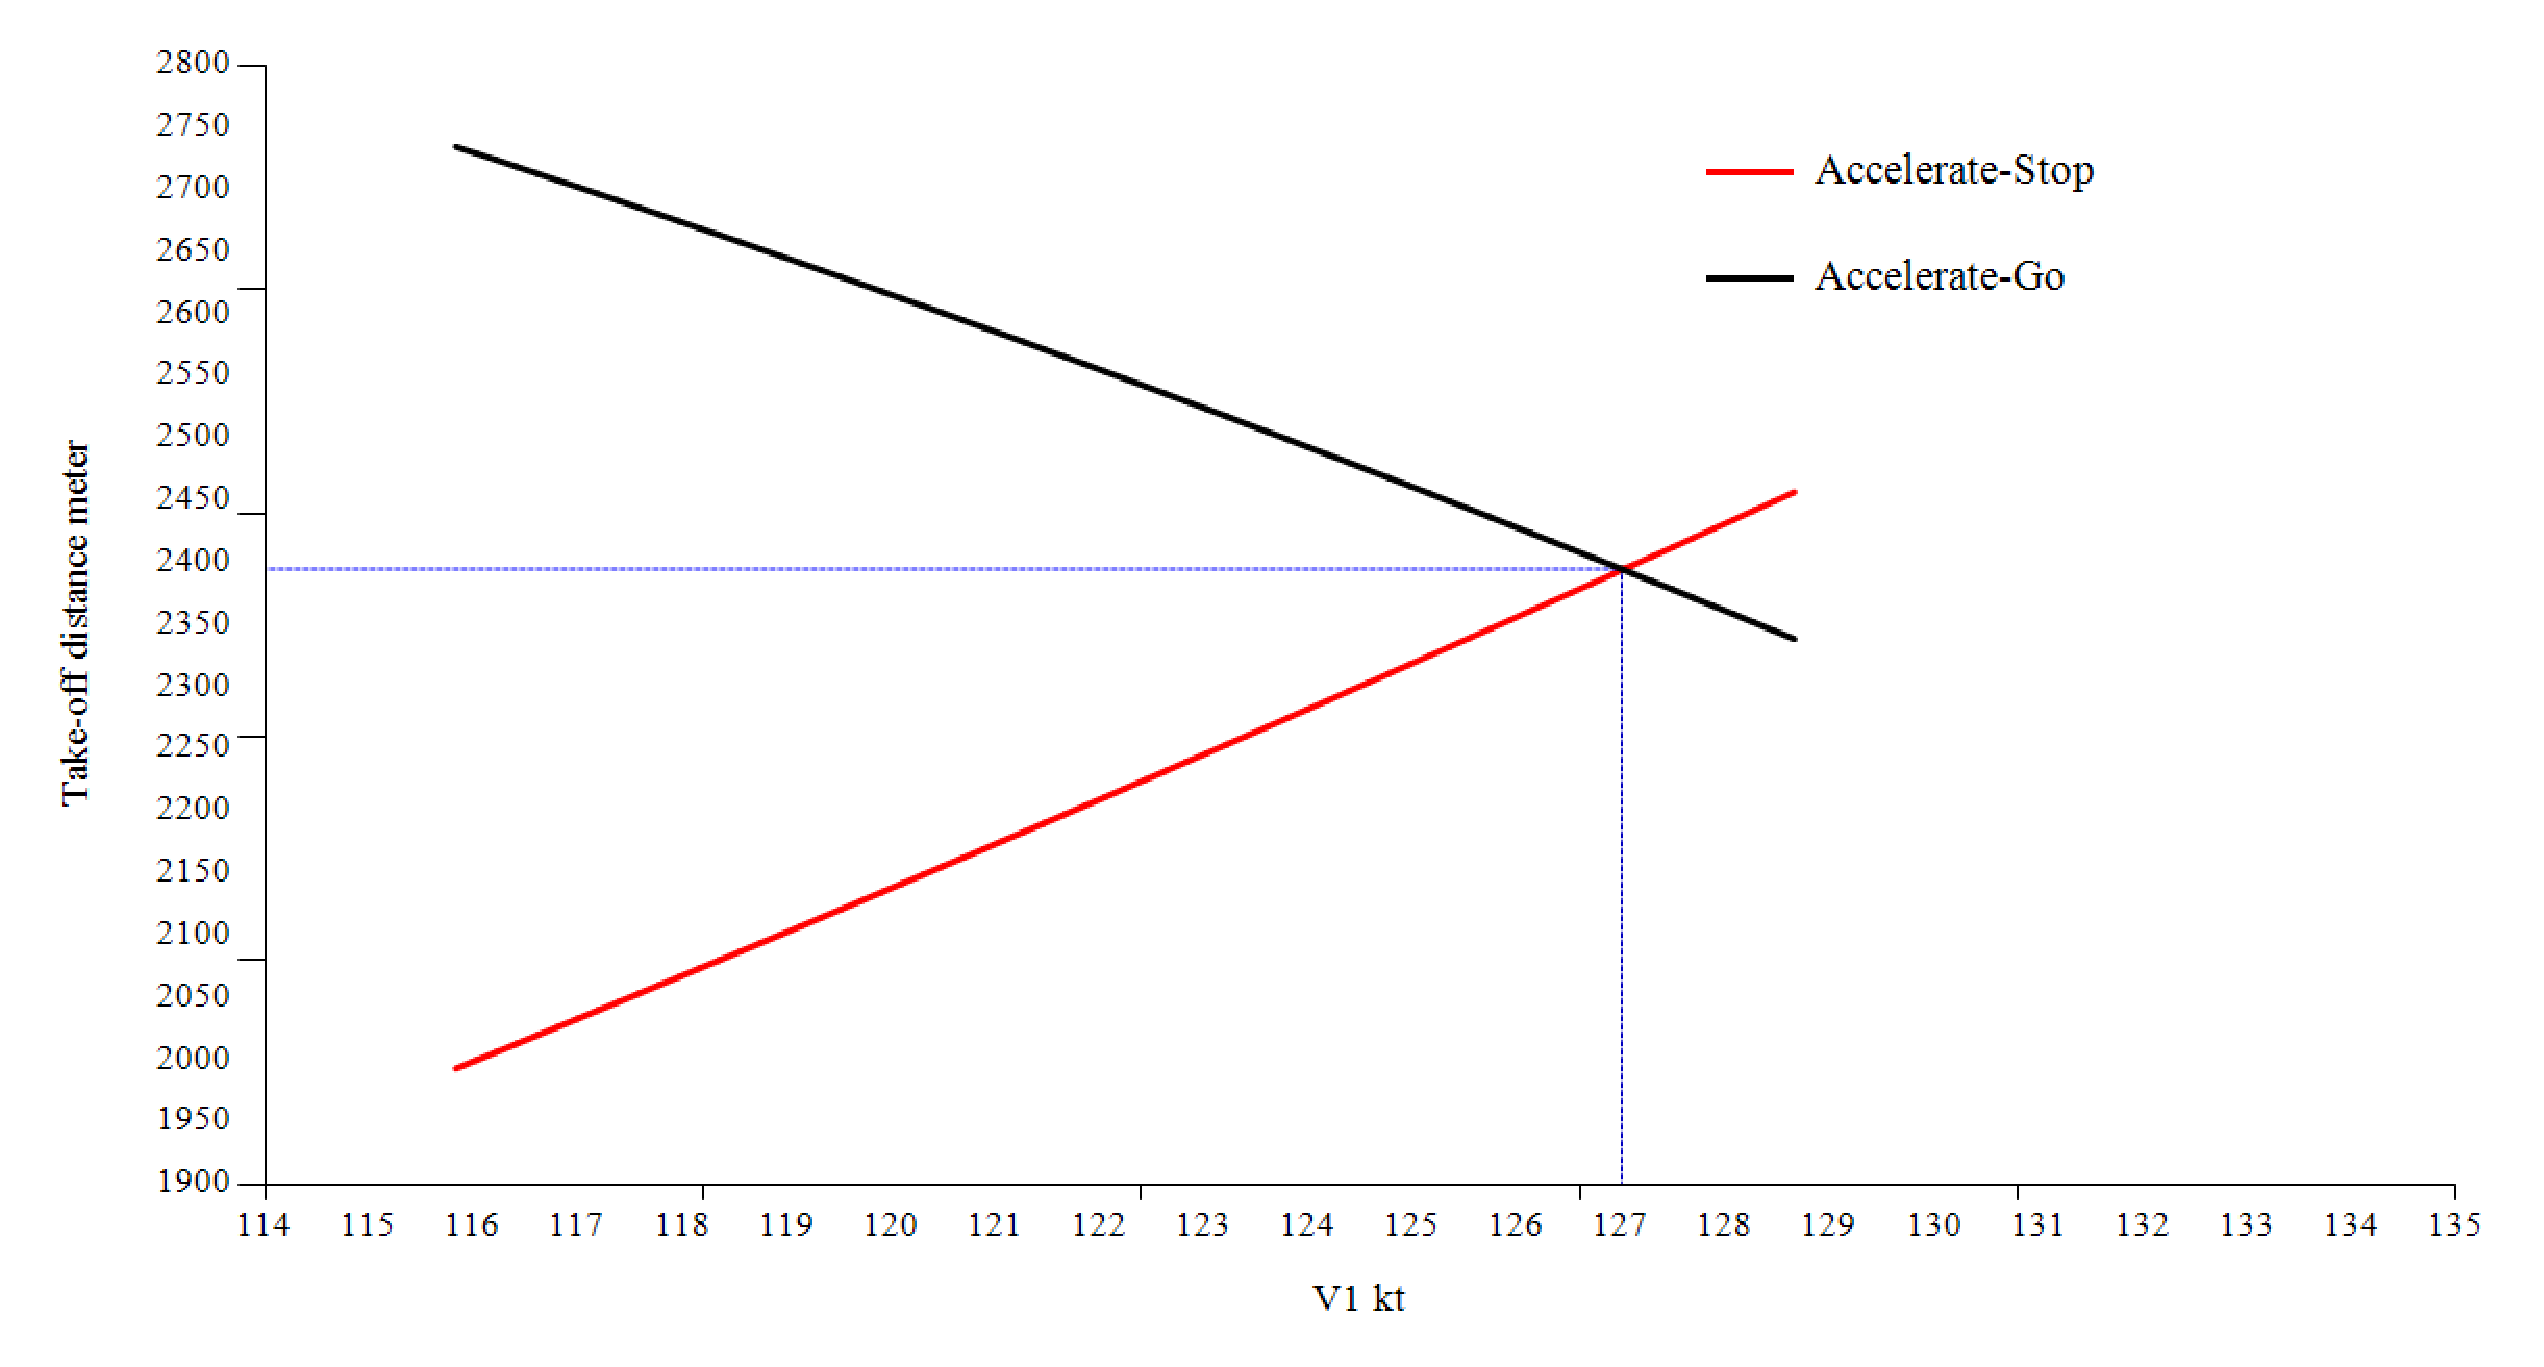
\includegraphics[width=0.9\textwidth]{pic/verifybfl.eps}\hspace{30pt}
	\caption{使用空客300-600验证平衡场长}\label{verifybfl}
\end{figure}


\chapter{仿真平台开发}

\section{仿真平台简述}

第\ref{highspeedperformance}、\ref{lowspeedperformance}章介绍了计算民航飞机性能数据的方法及根据这些方法编写的性能计算代码。所有计算函数均在Aircraft类中,主程序输入参数后进行调用即可输出计算得到的性能数据。

开发仿真平台可以填补飞机性能教学中缺少的可视化实证数据。在飞机性能工程课程的学习中,关于各种曲线和图像的推导基本来自定性分析,即从分析得到的曲线趋势推断整个曲线。而课本给出的曲线图均从飞机运行手册上直接摘录,无法获知图中的具体性能数据,也不能修改参数得到不同情况下的曲线。为弥补这些缺陷,以Aircraft作为基本类开发一款仿真平台,利用计算函数输出的数据制作性能图表。这些图表涵盖了大多数性能工程课程中所用图表,如推力线图、速度包线图等。

考虑到平台软件使用的便捷性,采用C\#语言制作WPF界面,利用其内部控件完成图表的绘制工作。平台还提供了参数调节功能,使用者在绘制性能图表时可以自行指定参数,输出该参数下的性能曲线。


\section{仿真平台设计}

软件平台使用Aircraft类计算得到的性能数据,根据性能工程中的相关公式编程制作性能图册\cite{PerformaceCourse}。绘制的图册包括气动特性、分析性能方法、飞机运行边界、起飞阶段、爬升阶段、巡航阶段及下降阶段中所用到的图表。本节展示的图片为空客300-600的性能图表,使用的基本参数为BADA 3.7提供的该机型数据。

\subsection{气动特性}\label{Dcurve}

(1)极曲线

根据式\ref{CDrag}绘制极曲线。由升阻比$k$

\begin{equation}
k=\frac{L}{D}=\frac{C_{\rm L}}{C_{\rm D}}
\end{equation}

可知$k$为极曲线斜率。升阻比最小即斜率最小,在绘制极曲线时标注该点,如图\ref{dragpolar}所示。

\begin{figure}[h]
	\centering
	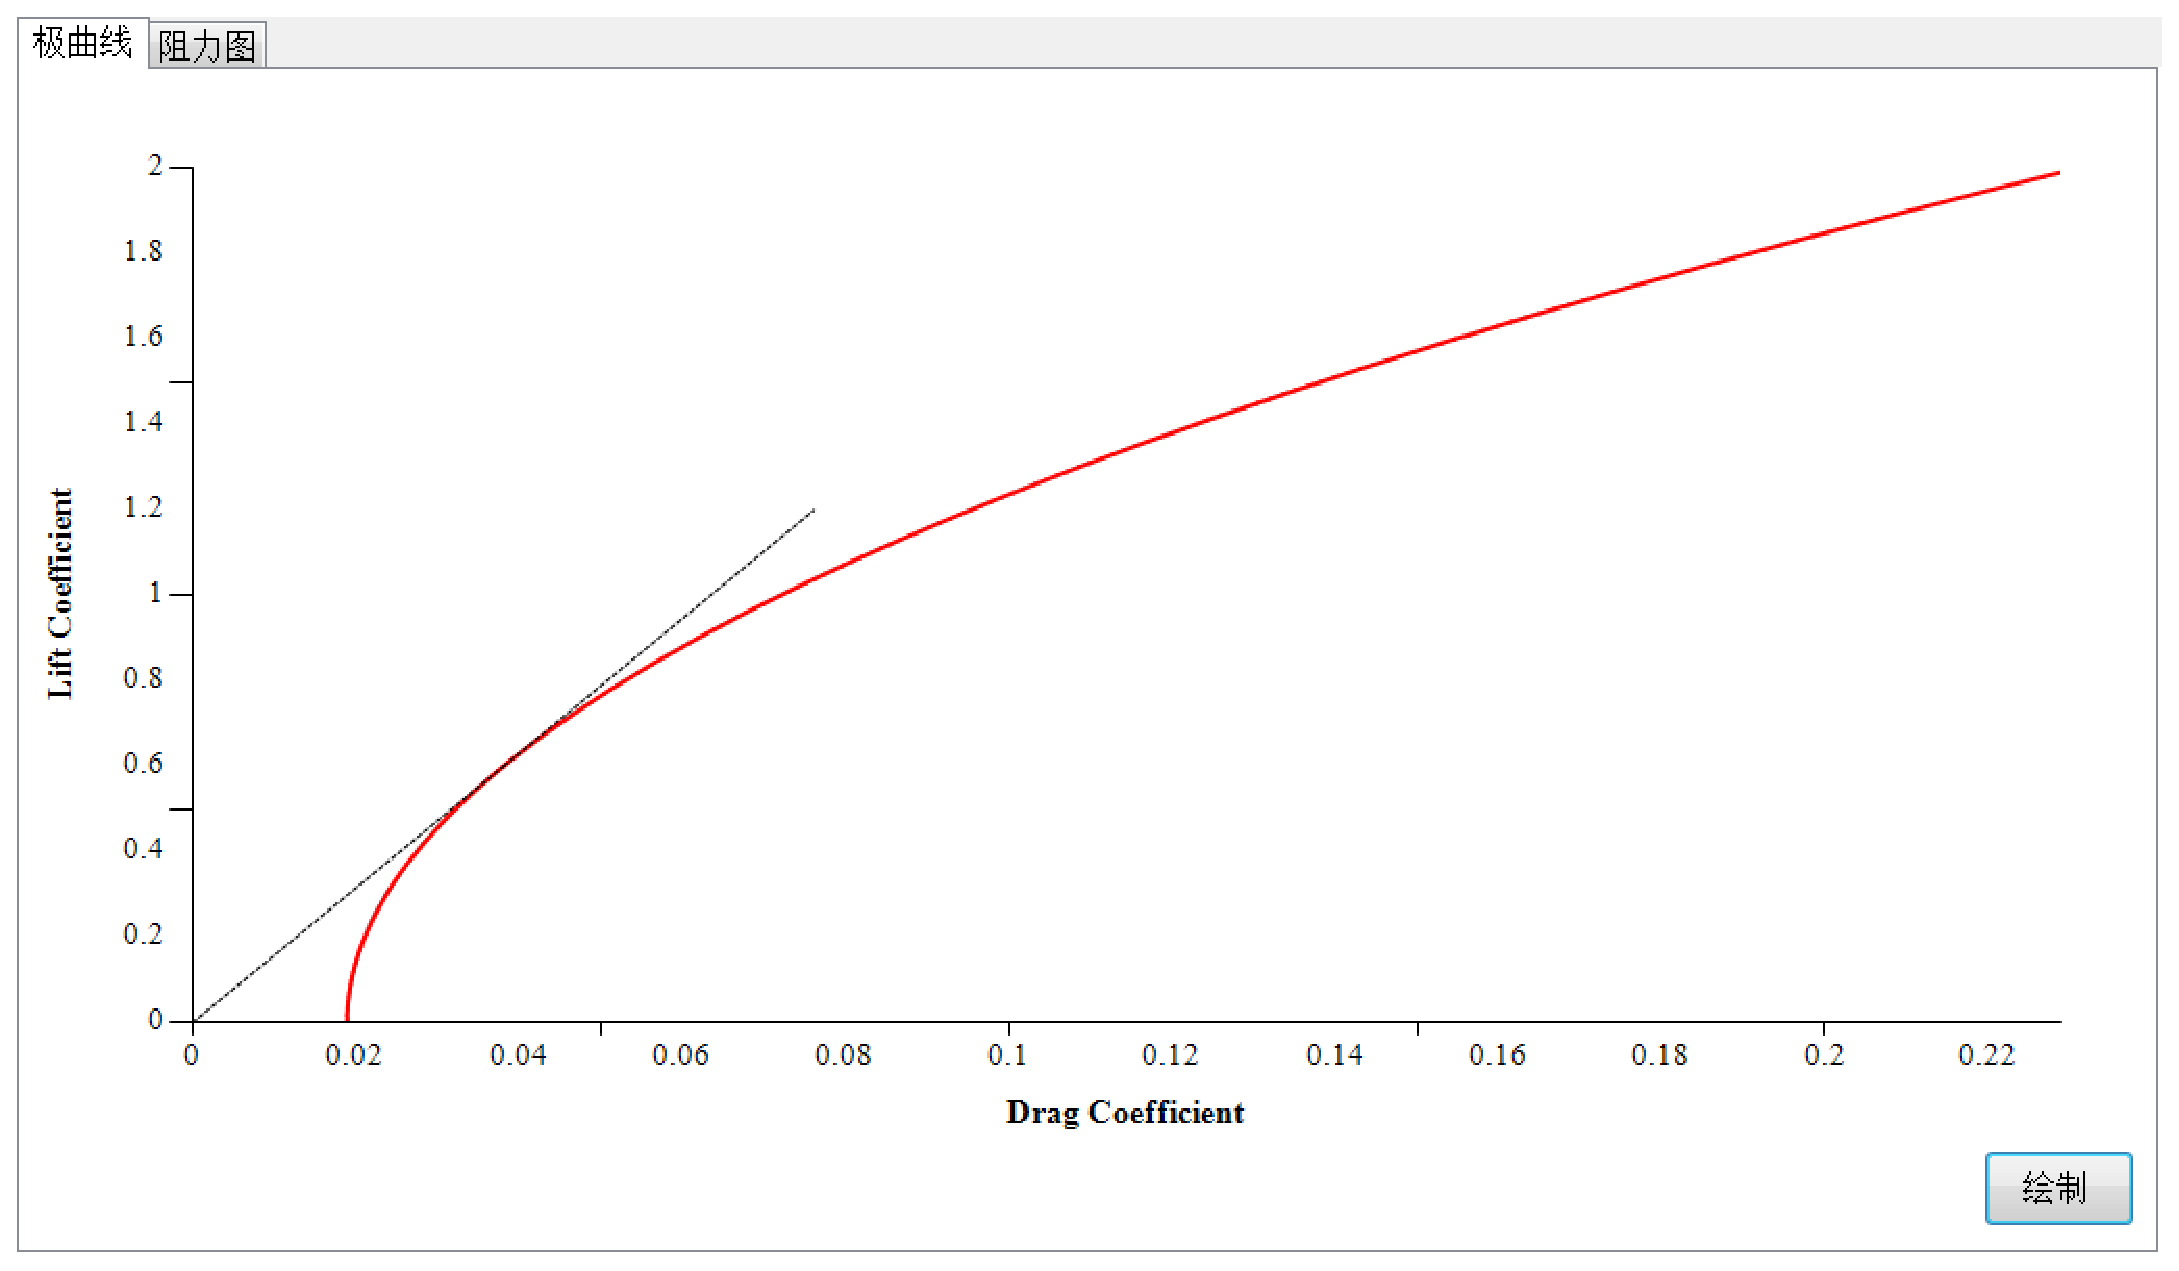
\includegraphics[width=0.8\textwidth]{pic/dragpolar.eps}\hspace{30pt}
	\caption{空客300-600极曲线}\label{dragpolar}
\end{figure}

(2)阻力图($D$\ - $v_{\rm TAS}$曲线)

在探讨阻力成因时,可将阻力$D$分为两部分:寄生阻力$D_{\rm parasite}$和诱导阻力$D_{\rm induced}$。由

\begin{equation}\label{Ddis}
D=\frac{1}{2}\rho v_{\rm TAS}^2 S C_{\rm D}
\end{equation}

及

\begin{equation}\label{CDtoD}
C_{\rm D}=A+B\cdot C_{\rm L}^2
\end{equation}

将式\ref{CDtoD}代入式\ref{Ddis},有

\begin{equation}\label{Ddeduce}
D=\frac{1}{2}\rho S\left(A\cdot v_{\rm TAS}^2+B\cdot v_{\rm TAS}^2 C_{\rm L}^2\right)
\end{equation}

由于在定常飞行中升力$L$与航空器重力$W$相等,即

\begin{equation}\label{L_CL}
L=\frac{1}{2}\rho v_{\rm TAS}^2 S C_{\rm L}=W
\end{equation}

假定航空器重力$W$为已知量,则将式\ref{L_CL}代入式\ref{Ddeduce}:

\begin{equation}
\begin{split}
D&=\frac{1}{2}\rho S\left[A\cdot v_{\rm TAS}^2+B\cdot v_{\rm TAS}^2\frac{W^2}{\left(\frac{1}{2}\rho v_{\rm TAS}^2 S\right)^2}\right]\\
&=\frac{1}{2}\rho S\left(A\cdot v_{\rm TAS}^2+B\frac{W^2}{\frac{1}{4}\rho^2 S^2 v_{\rm TAS}^2}\right)\\
&=\frac{1}{2}\rho S v_{\rm TAS}^2+\frac{1}{2}B\frac{4W^2}{\rho S v_{\rm TAS}^2}\\
&=\frac{1}{2}A\rho S v_{\rm TAS}^2+2B\frac{W^2}{\rho S}\frac{1}{v_{\rm TAS}^2}
\end{split}
\end{equation}

因为寄生阻力随速度增加而增加,诱导阻力随速度增加而减小,故从上式可以看出

\begin{equation}
D_{\rm parasite}=\frac{1}{2}A\rho S v_{\rm TAS}^2
\end{equation}

\begin{equation}
D_{\rm induced}=2B\frac{W^2}{\rho S}\frac{1}{v_{\rm TAS}^2}
\end{equation}

为了验证阻力$D$确实由这两部分阻力组成,即

\begin{equation}
D=D_{\rm parasite}+D_{\rm induced}
\end{equation}

绘制这两部分阻力及总阻力随速度变化的曲线,如图\ref{dragcurve}所示。结果显示正是由于寄生阻力随速度增加而增大、诱导阻力随速度增加而减少,才使得总阻力随速度增大的变化趋势为先减小后增大。

\begin{figure}[h]
	\centering
	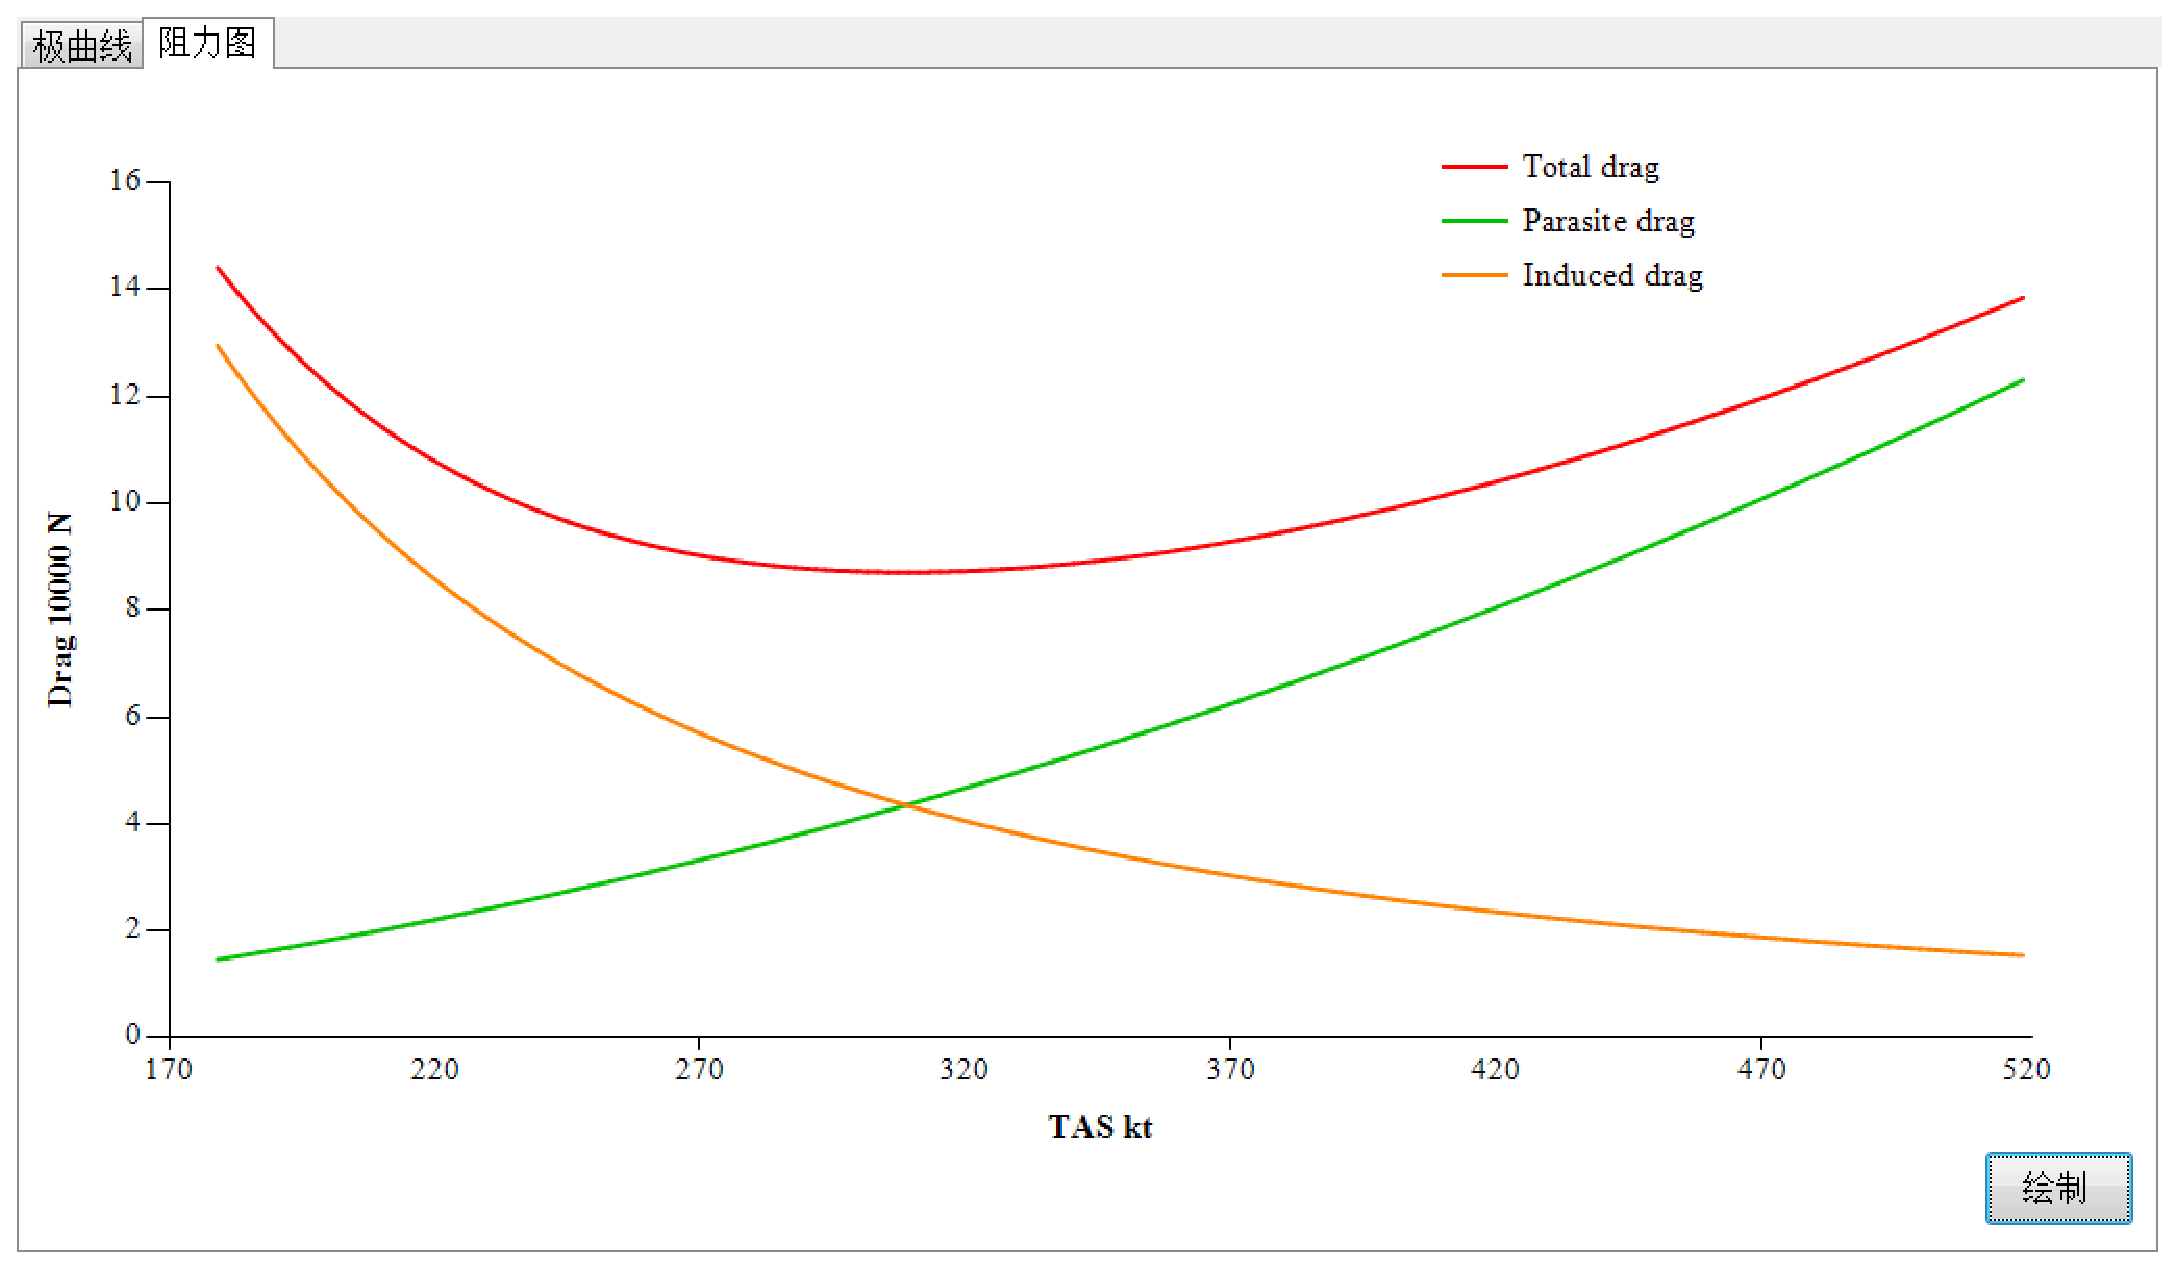
\includegraphics[width=0.8\textwidth]{pic/drag.eps}\hspace{30pt}
	\caption{空客300-600阻力图}\label{dragcurve}
\end{figure}

\subsection{分析性能方法}

(1)推力法

($\romannumeral1$)所需推力曲线随重量的变化

绘制空客300-600飞机在18000 $\rm ft$上的所需推力曲线,并改变重量参数继续绘制。如图\ref{FRwithW}所示,可以看到随着重量增加,曲线逐渐向右上方移动。

\begin{figure}[h]
	\centering
	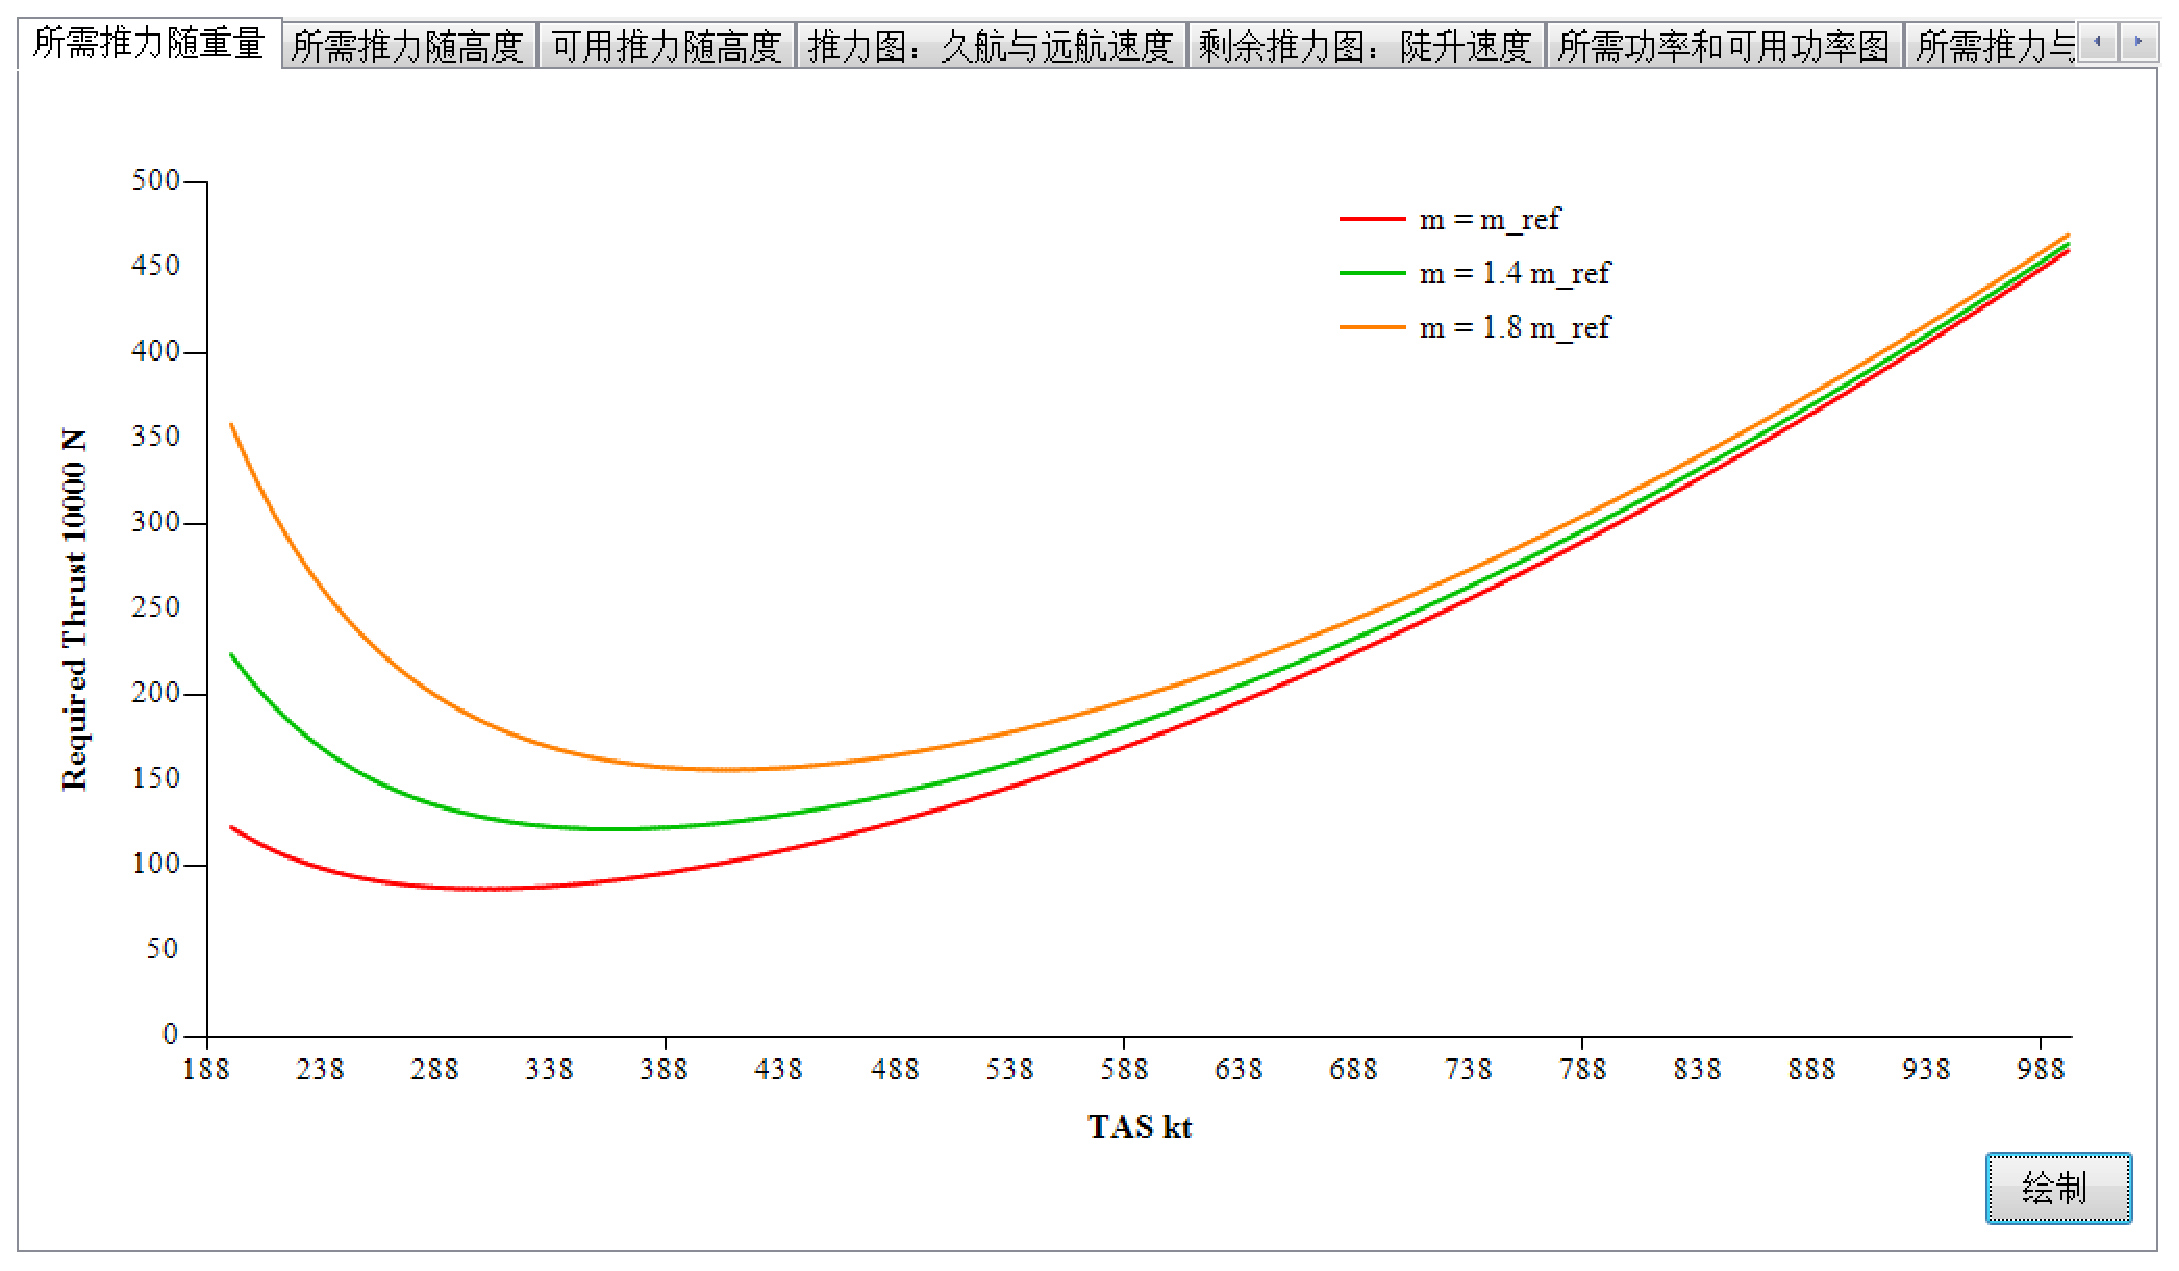
\includegraphics[width=0.8\textwidth]{pic/FRwithW.eps}\hspace{30pt}
	\caption{空客300-600所需推力随重量曲线}\label{FRwithW}
\end{figure}

($\romannumeral2$)所需推力曲线随高度的变化

绘制空客300-600飞机在参考重量(140 $\rm t$)时的所需推力曲线,并改变高度参数继续绘制。如图\ref{FRwithh}所示,可以看到随着高度升高,曲线逐渐向右移动。

\begin{figure}[h]
	\centering
	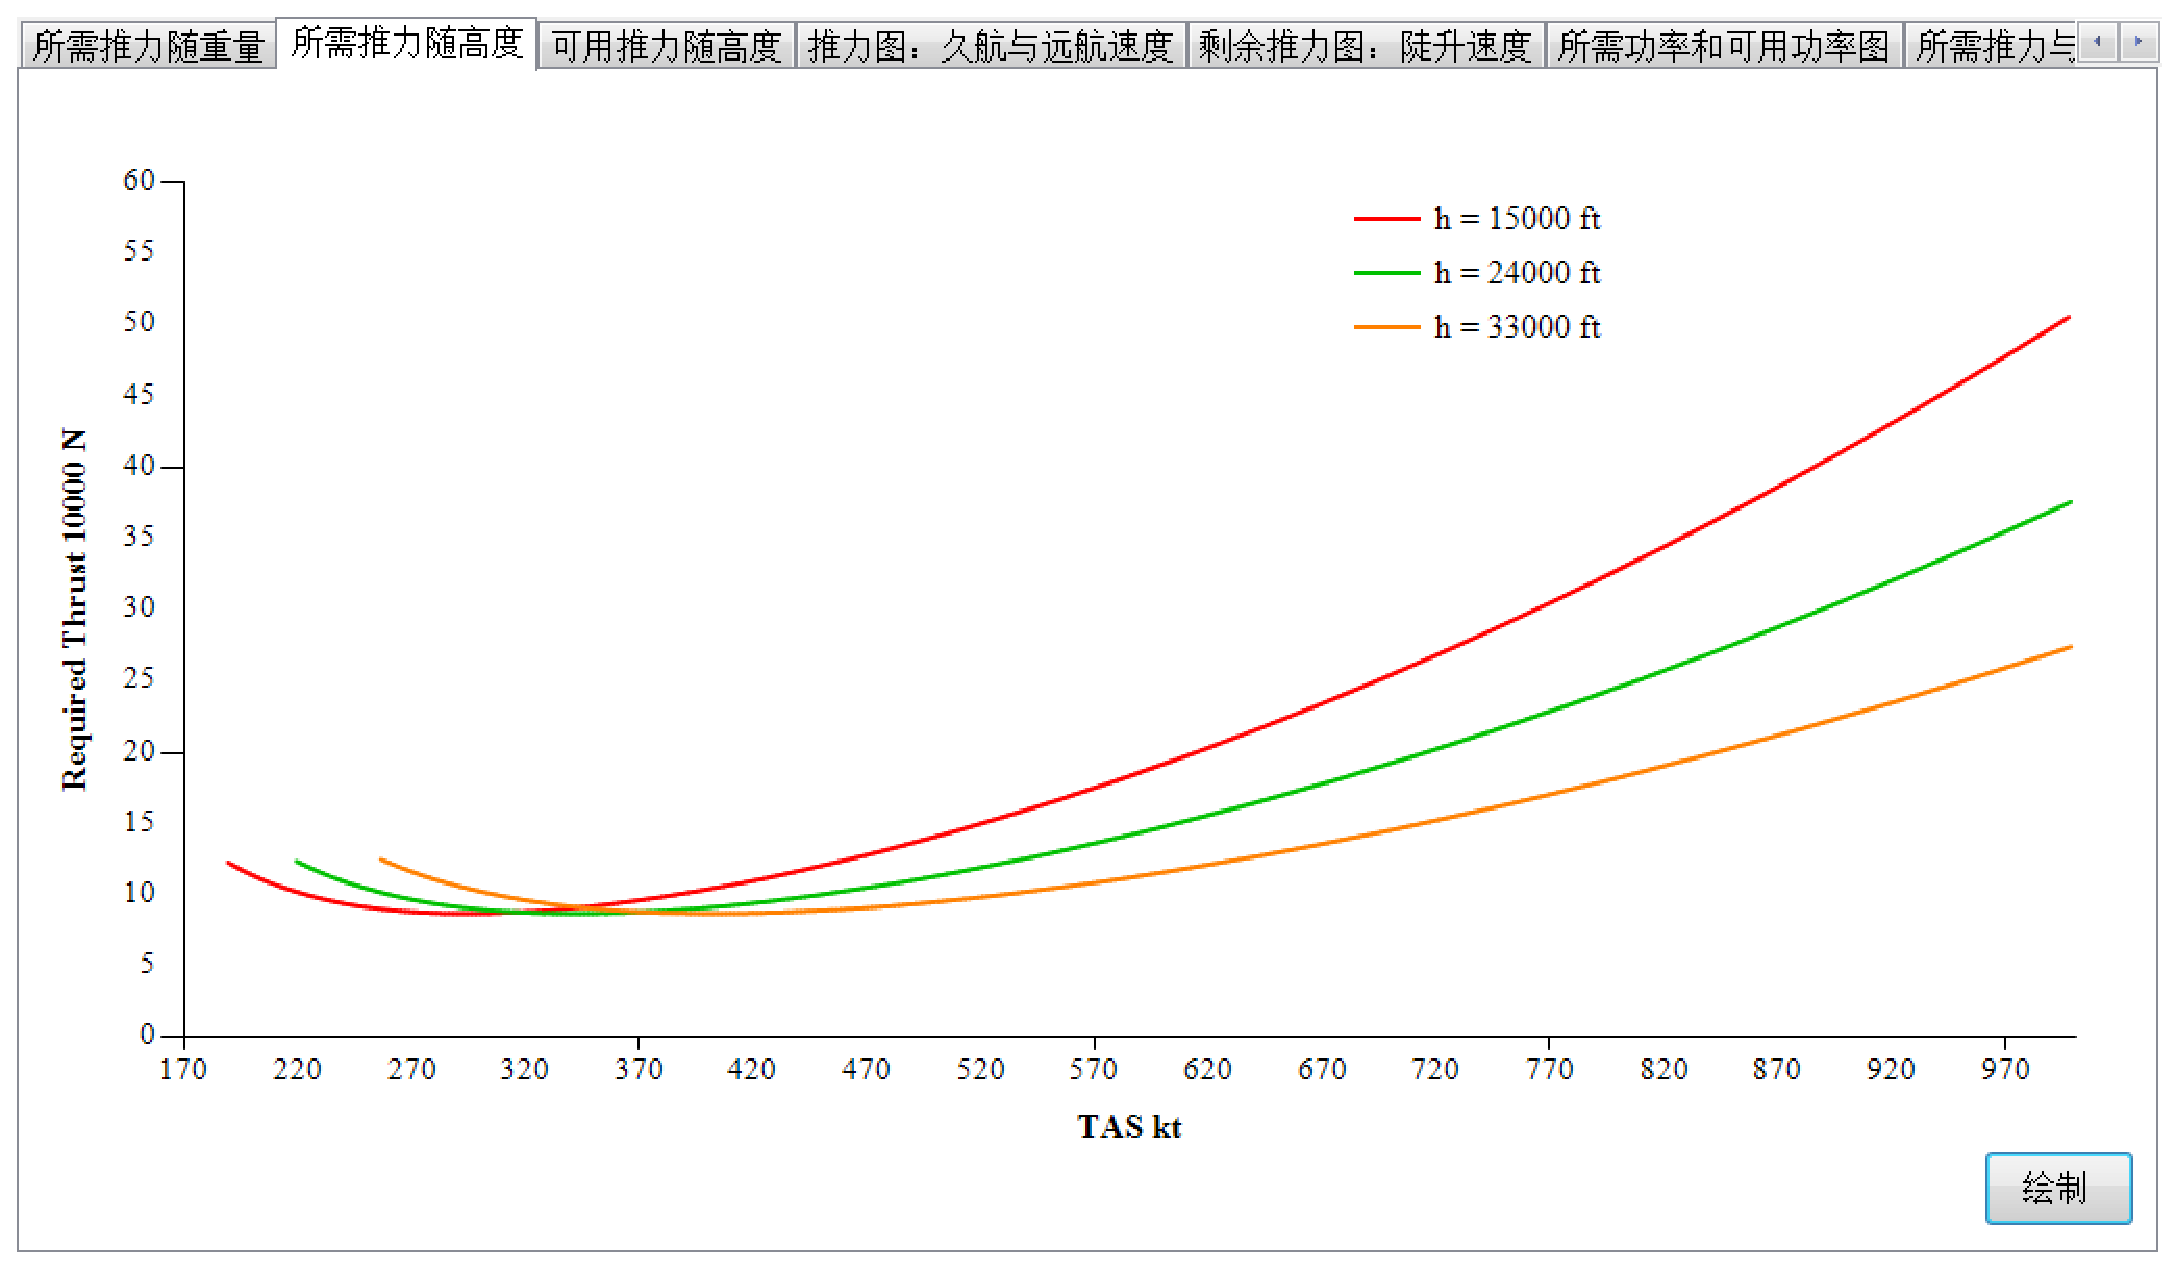
\includegraphics[width=0.8\textwidth]{pic/FRwithh.eps}\hspace{30pt}
	\caption{空客300-600所需推力随高度曲线}\label{FRwithh}
\end{figure}



($\romannumeral3$)可用推力曲线随高度的变化

绘制空客300-600飞机在参考重量(140 $\rm t$)时的可用曲线,并改变高度参数继续绘制。如图\ref{Fawithh}所示,可以看到随着高度升高,曲线逐渐向下移动。

\begin{figure}[h]
	\centering
	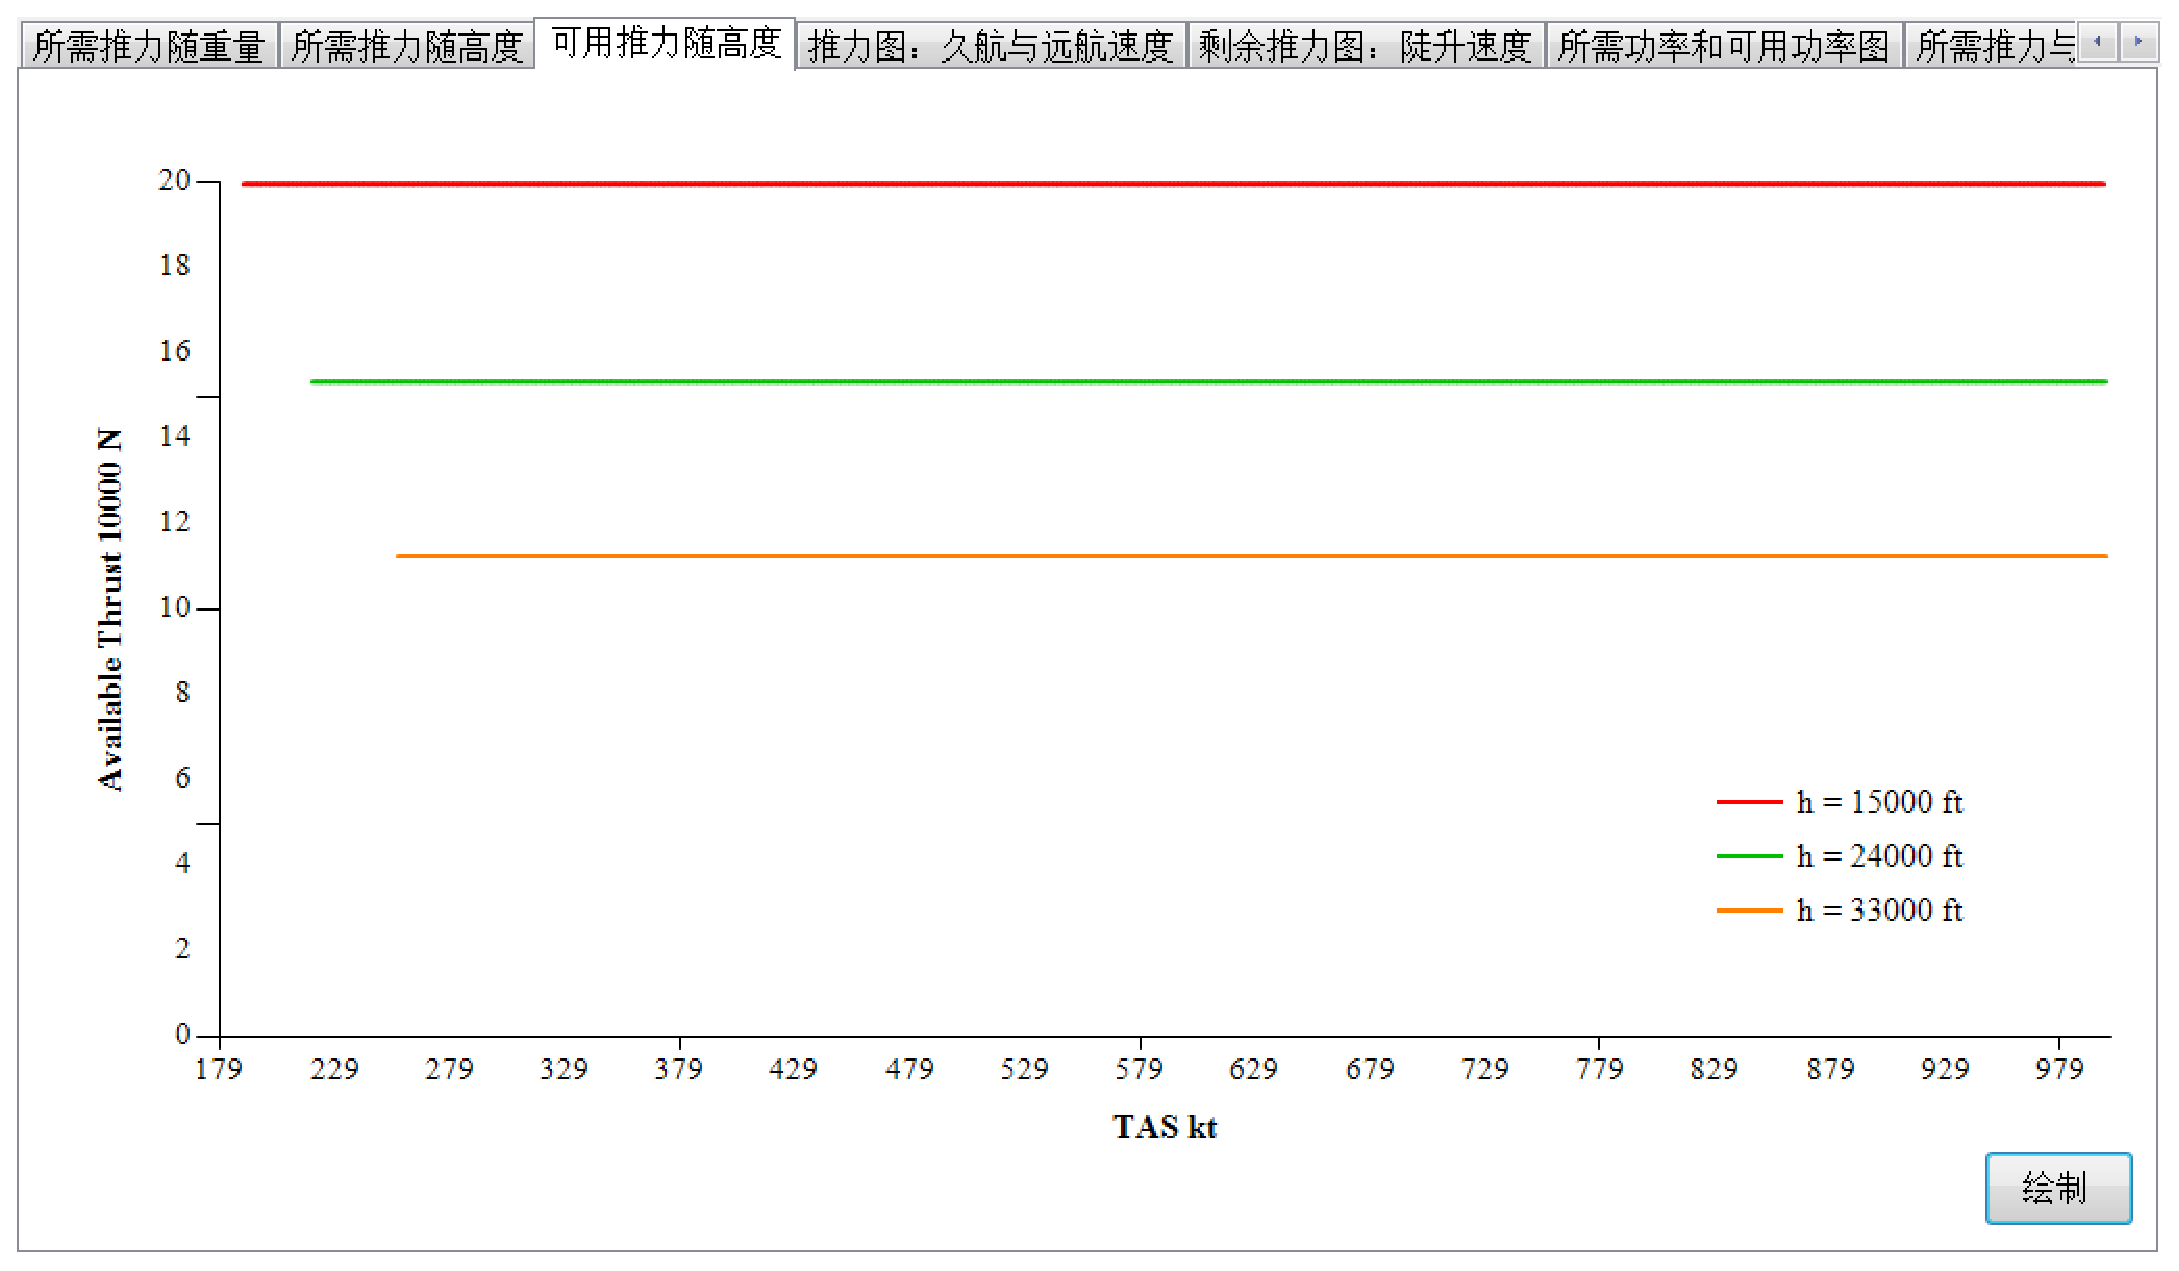
\includegraphics[width=0.8\textwidth]{pic/Fawithh.eps}\hspace{30pt}
	\caption{空客300-600可用推力随高度曲线}\label{Fawithh}
\end{figure}




($\romannumeral4$)推力图中的久航速度和远航速度

根据性能工程的知识,航空器燃油流量$ff$最小时的速度为久航速度。该速度也被称为有利速度。由燃油流量公式

\begin{equation}\label{ff}
ff=TSFC\times F_{\rm N}
\end{equation}

式中$TSFC$是单位时间单位推力耗油量,为定值。$F_{\rm N}$为所需推力。若要燃油流量$ff$最小,需要所需推力最小,即所需推力曲线的最低点对应速度为久航速度。

远航速度为飞机以此速度飞行的距离最长。考察燃油里程$SR$

\begin{equation}\label{SRequ}
SR=\frac{v_{\rm TAS}}{ff}
\end{equation}

将式\ref{ff}代入,得到

\begin{equation}
SR=\frac{1}{TSFC}\frac{v_{\rm TAS}}{F_{\rm N}}
\end{equation}

若要燃油里程$SR$最大,则需$\displaystyle{\frac{v_{\rm TAS}}{F_{\rm N}}}$最大。对其取倒数,即

\begin{equation}
\frac{v_{\rm TAS}}{F_{\rm N}}=\left(\frac{F_{\rm N}}{v_{\rm TAS}}\right)^{-1}
\end{equation}

当$\displaystyle{\frac{F_{\rm N}}{v_{\rm TAS}}}$最小时$SR$取得最大值。注意到$\displaystyle{\frac{F_{\rm N}}{v_{\rm TAS}}}$为所需推力曲线斜率,故在斜率最小点处的速度即为远航速度。

绘制空客300-600飞机在18000 $\rm ft$上的所需推力和可用推力曲线,形成推力图,并在图中标注久航速度$v_{\rm long-duration}$和远航速度$v_{\rm MRC}$,如图\ref{vlongduranceandmrc}所示。

\begin{figure}[h]
	\centering
	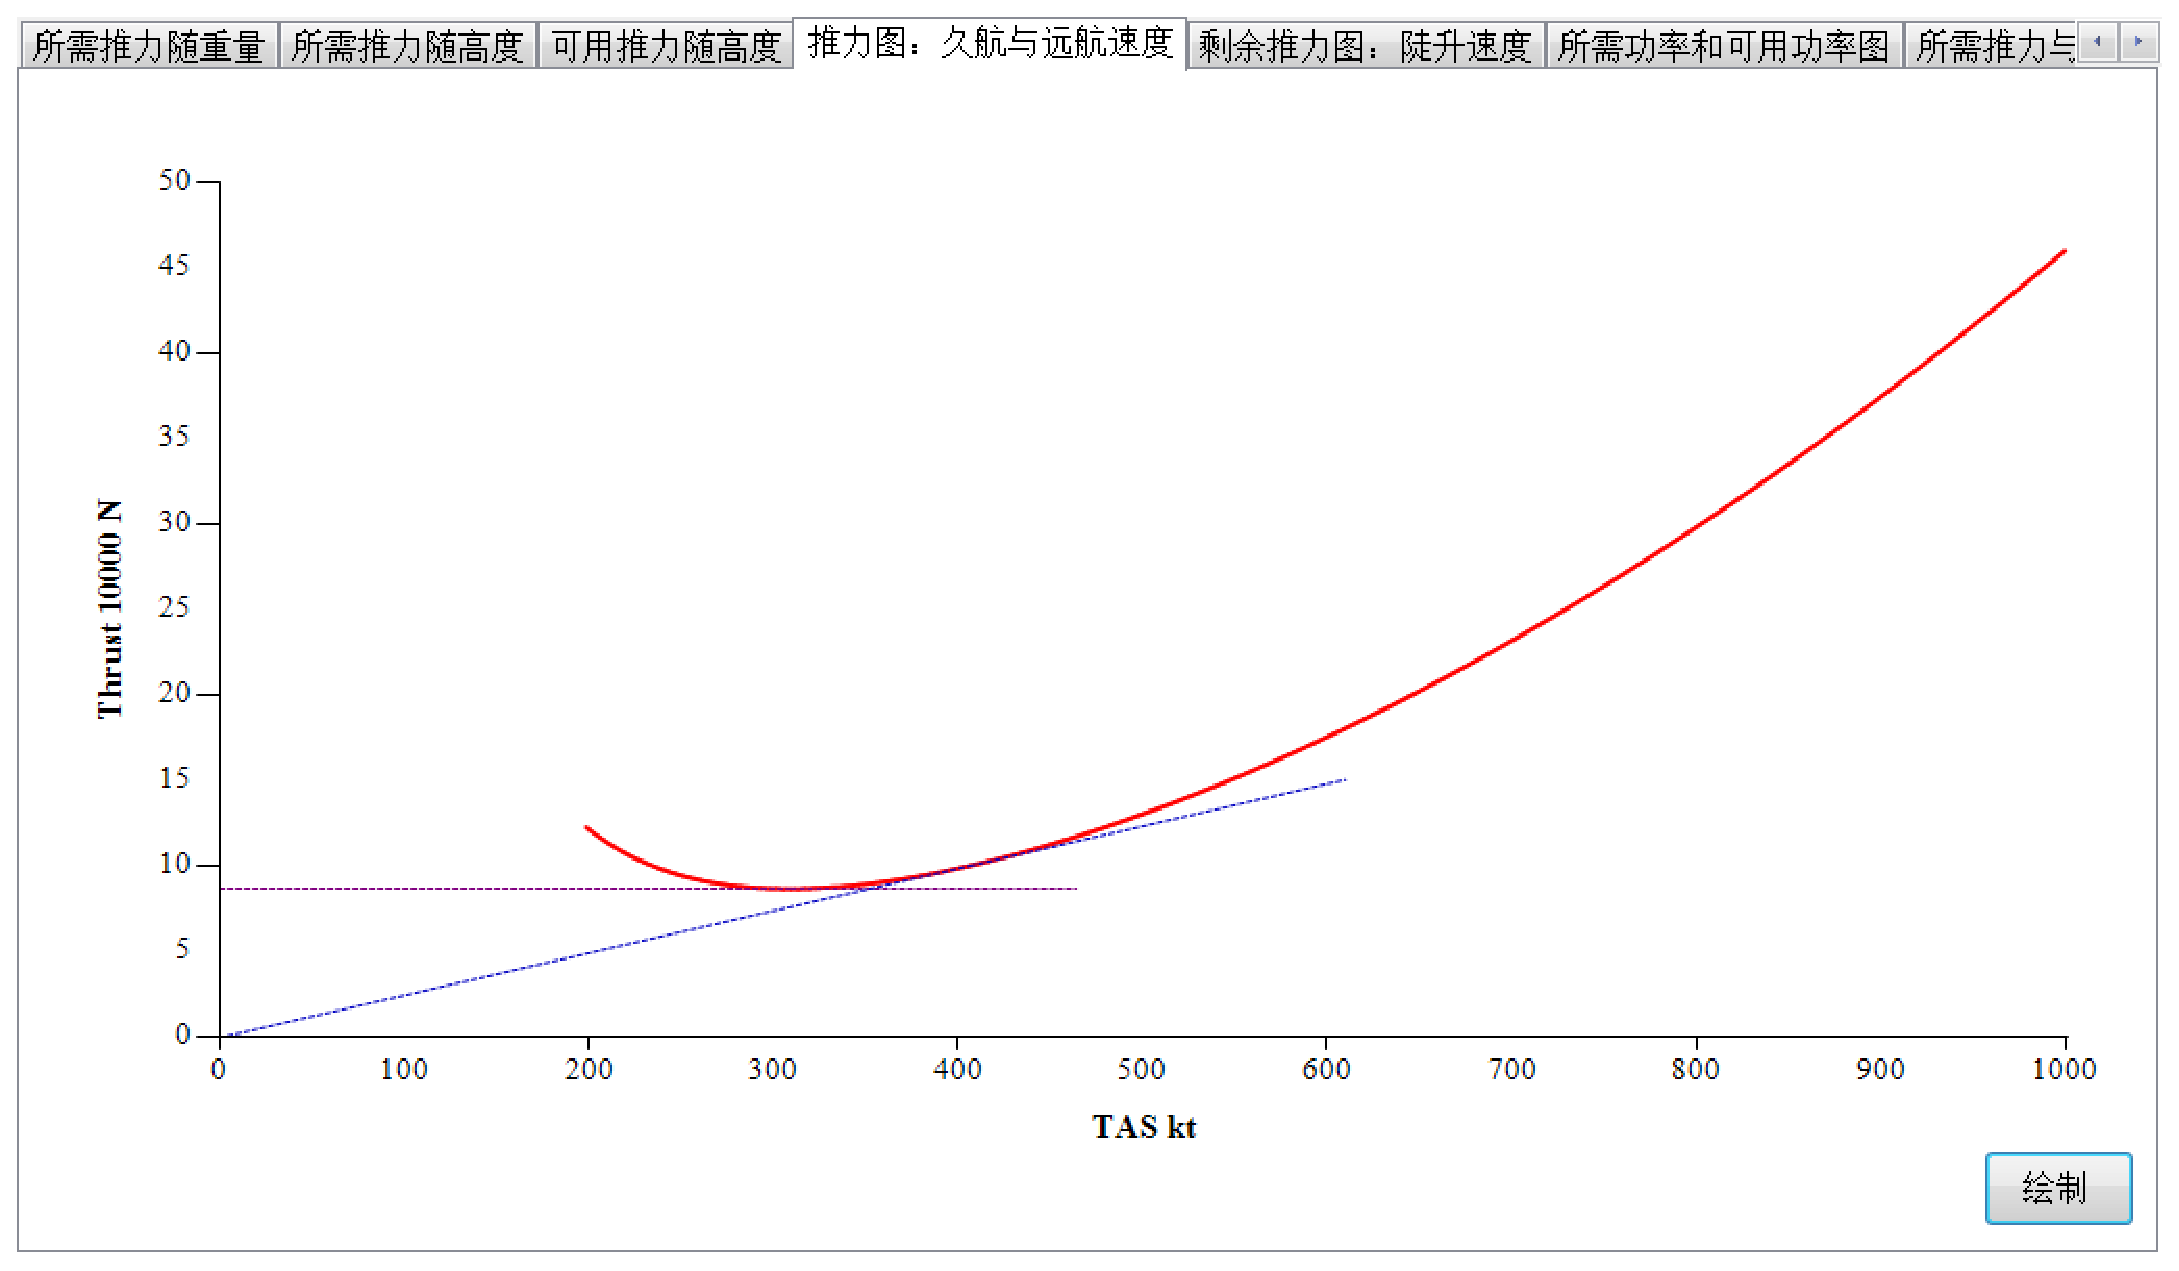
\includegraphics[width=0.8\textwidth]{pic/vlongduranceandmrc.eps}\hspace{30pt}
	\caption{空客300-600推力图中久航速度和远航速度}\label{vlongduranceandmrc}
\end{figure}




($\romannumeral5$)剩余推力图中的陡升速度

剩余推力$F_{\rm redundant}$为

\begin{equation}
F_{\rm redundant}=F{\rm a}-F_{\rm N}
\end{equation}

其中$F{\rm a}$为可用推力,$F_{\rm N}$为所需推力。

飞机以陡升速度爬升,其爬升梯度最大。爬升梯度$\sin\theta$

\begin{equation}\label{sintheta}
\sin\theta=\frac{F_{\rm redundant}}{W}
\end{equation}

则当航空器重量$W$一定时,爬升梯度最大需要剩余推力$F_{\rm redundant}$最大,该点对应速度为陡升速度。

绘制空客300-600飞机在28000 $\rm ft$上的剩余推力曲线,找到其中的陡升速度,如图\ref{vsteepclimbinredundantF}所示。

\begin{figure}[h]
	\centering
	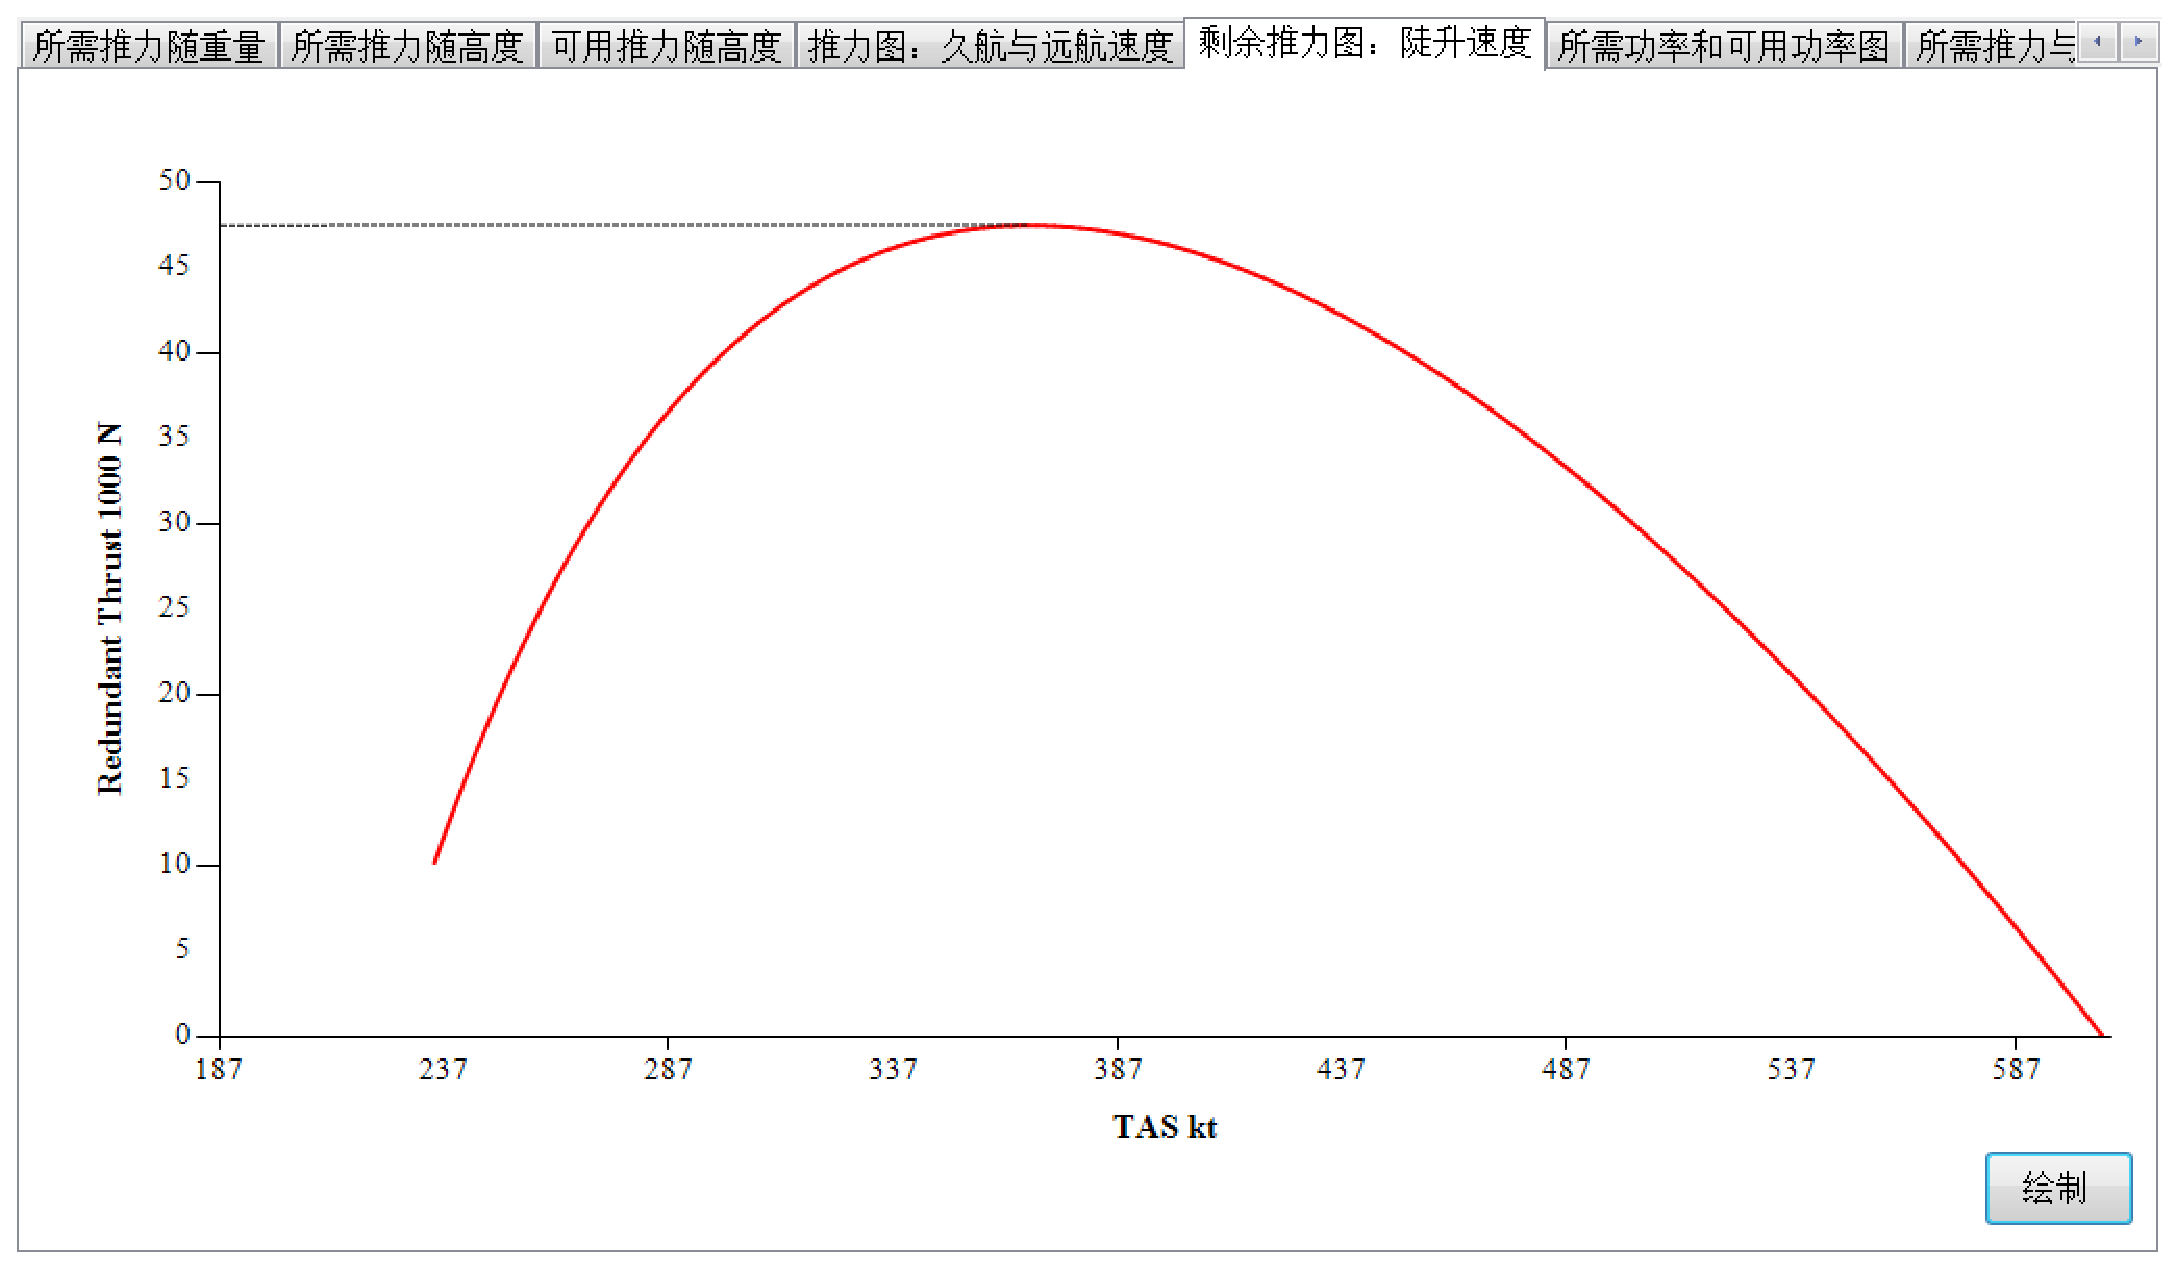
\includegraphics[width=0.8\textwidth]{pic/vsteepclimbinredundantF.eps}\hspace{30pt}
	\caption{空客300-600剩余推力图与陡升速度}\label{vsteepclimbinredundantF}
\end{figure}


(2)功率法

($\romannumeral1$)所需功率和可用功率曲线

由于功率为力与速度乘积,故有

\begin{equation}
W_{\rm N}=F_{\rm N}\times v_{\rm TAS}
\end{equation}

\begin{equation}
W_{\rm a}=F_{\rm a}\times v_{\rm TAS}
\end{equation}

绘制空客300-600飞机在18000\ $\rm ft$上的所需功率曲线和可用功率曲线,如图\ref{WRandWa}所示。

\begin{figure}[h]
	\centering
	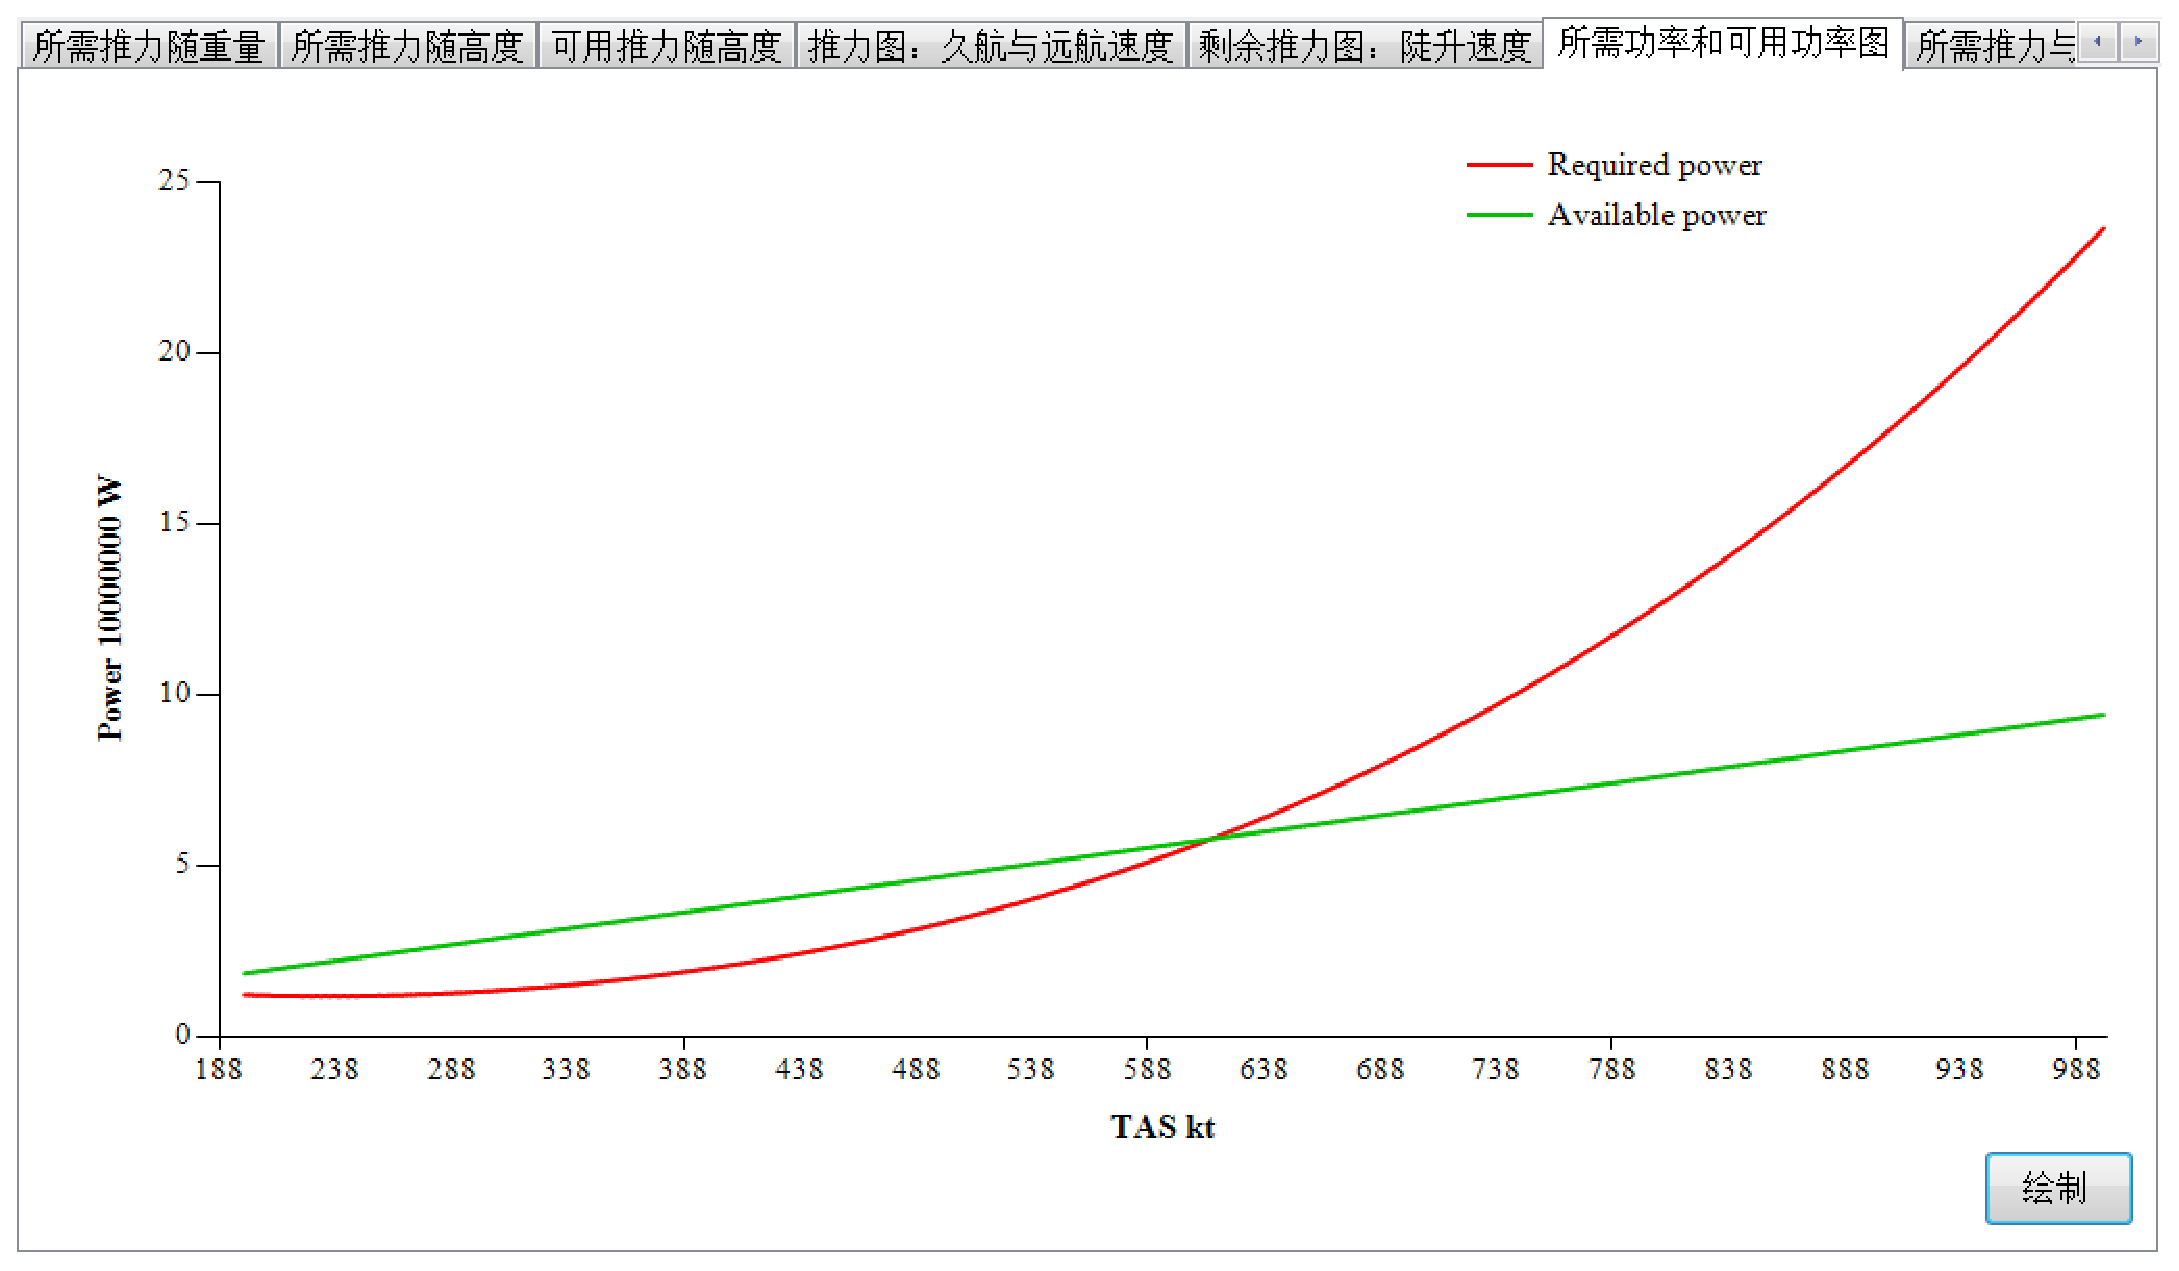
\includegraphics[width=0.8\textwidth]{pic/WRandWa.eps}\hspace{30pt}
	\caption{空客300-600所需功率与可用功率曲线}\label{WRandWa}
\end{figure}


($\romannumeral2$)所需推力曲线与所需功率曲线上的有利速度

在所需推力线上,有利速度为所需推力最小处的$v_{\rm TAS}$。而在所需功率曲线上,其斜率

\begin{equation}
slope_{\rm W_{\rm N}}=\frac{W_{\rm N}}{v_{\rm TAS}}=F_{\rm N}
\end{equation}

故有利速度在斜率最小点处取得。

绘制空客300-600飞机在32000 $\rm ft$上的所需推力曲线和所需功率曲线,并验证有利速度$v_{\rm e}$在两条曲线上的位置,如图\ref{veinFRandWR}所示。

\begin{figure}[h]
	\centering
	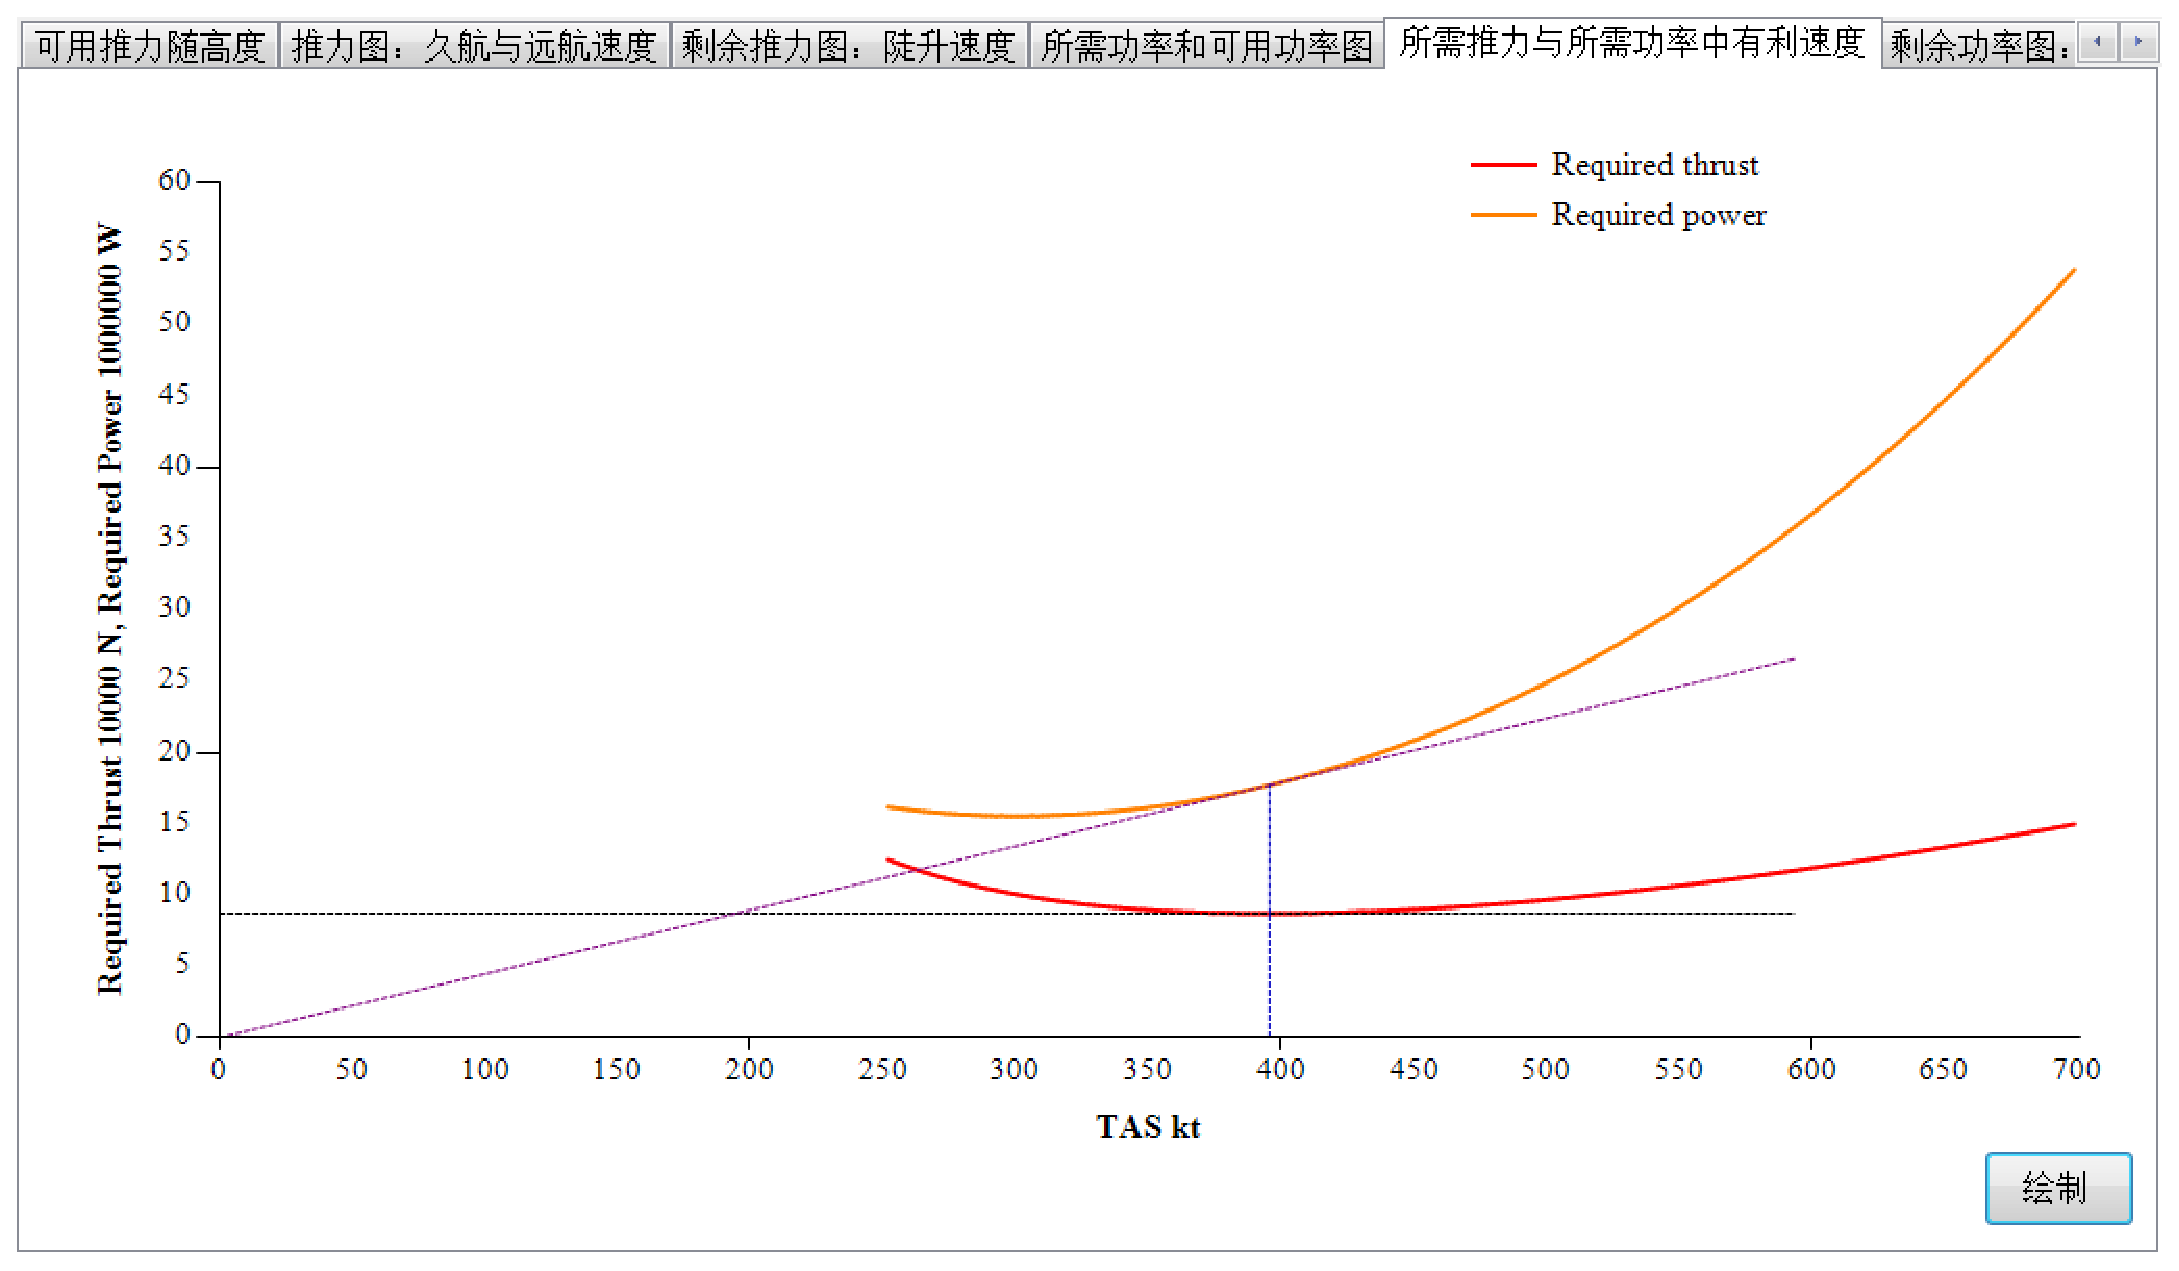
\includegraphics[width=0.8\textwidth]{pic/veinFRandWR.eps}\hspace{30pt}
	\caption{空客300-600所需推力与所需功率图中有利速度}\label{veinFRandWR}
\end{figure}



($\romannumeral3$)剩余功率图中的快升速度与陡升速度

飞机的剩余功率$W_{\rm redundant}$为

\begin{equation}
W_{\rm redundant}=W_{\rm a}-W_{\rm N}
\end{equation}

航空器以快升速度爬升的爬升率最大。由爬升率公式及式\ref{sintheta}

\begin{equation}\label{ROCD}
ROCD=v_{\rm TAS}\sin\theta=v_{\rm TAS}\frac{F_{\rm redundant}}{W}=\frac{W_{\rm redundant}}{W}
\end{equation}

若要爬升率最大,则需剩余功率最大,即快升速度为剩余功率曲线最高点的速度。

由前面的叙述已经知道,陡升速度为爬升梯度最大的速度,在剩余推力最大时取得。考虑剩余推力曲线斜率

\begin{equation}
slope_{\rm W_{redundant}}=\frac{W_{\rm redundant}}{v_{\rm TAS}}=\frac{F_{\rm redundant}\times v_{\rm TAS}}{v_{\rm TAS}}=F_{\rm redundant}
\end{equation}

则剩余功率曲线上斜率最小点处的速度为陡升速度。

绘制空客300-600飞机在18000 $\rm ft$上的剩余功率曲线,在图中找到快升速度$v_{\rm fast-climb}$与陡升$v_{\rm steep-climb}$速度,如图\ref{vfastclimbsteepclimbinredundantW}所示。

\begin{figure}[h]
	\centering
	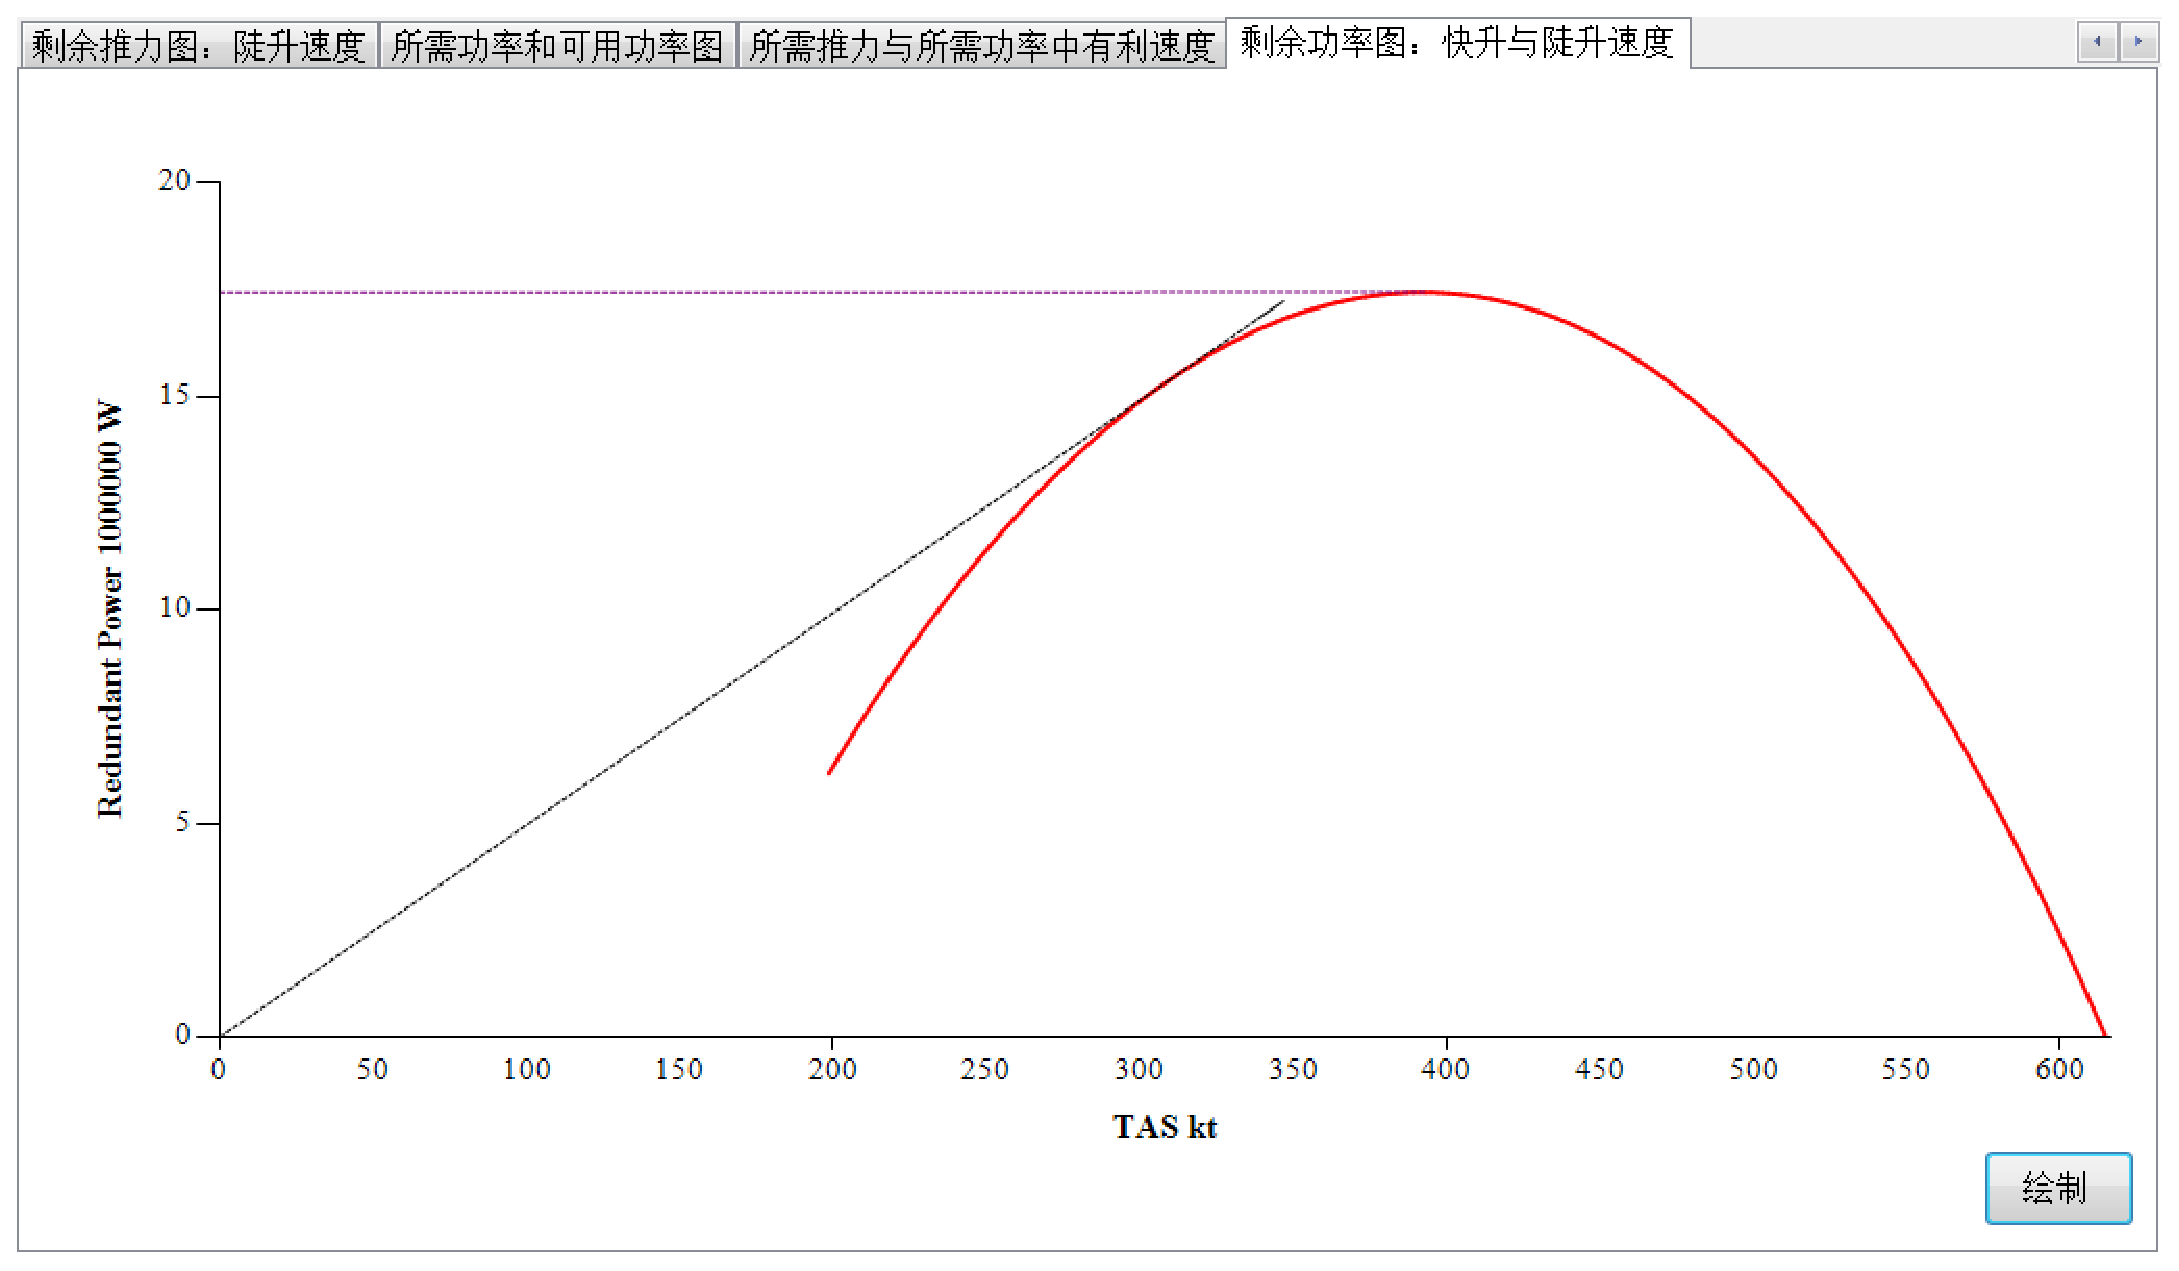
\includegraphics[width=0.8\textwidth]{pic/vfastclimbsteepclimbinredundantW.eps}\hspace{30pt}
	\caption{空客300-600剩余功率图中快升速度和陡升速度}\label{vfastclimbsteepclimbinredundantW}
\end{figure}

\subsection{飞机运行边界}

(1)所需推力、可用推力曲线随高度变化的左右交点

由前所述,随着高度升高,所需推力曲线右移、可用推力线下移,造成两条曲线产生左右交点。

飞机在低空时,所能飞的最小速度为失速速度$v_{\rm stall}$,而在高空所需推力曲线和可用推力曲线产生左交点,这点的左边剩余推力为负值,故在高空所能飞的最小速度为左交点对应的速度。同理,飞机能飞的最大速度为两条推力曲线右交点的速度。

绘制空客300-600飞机在15000 $\rm ft$与在32000 $\rm ft$上的推力图。在低空两条曲线只有右交点,飞机能飞的最小速度为失速速度,最大速度为右交点,而在高空最小速度为推力线的左交点,如图\ref{leftrightcrosspointinF-V}所示。


\begin{figure}[h]
	\centering
	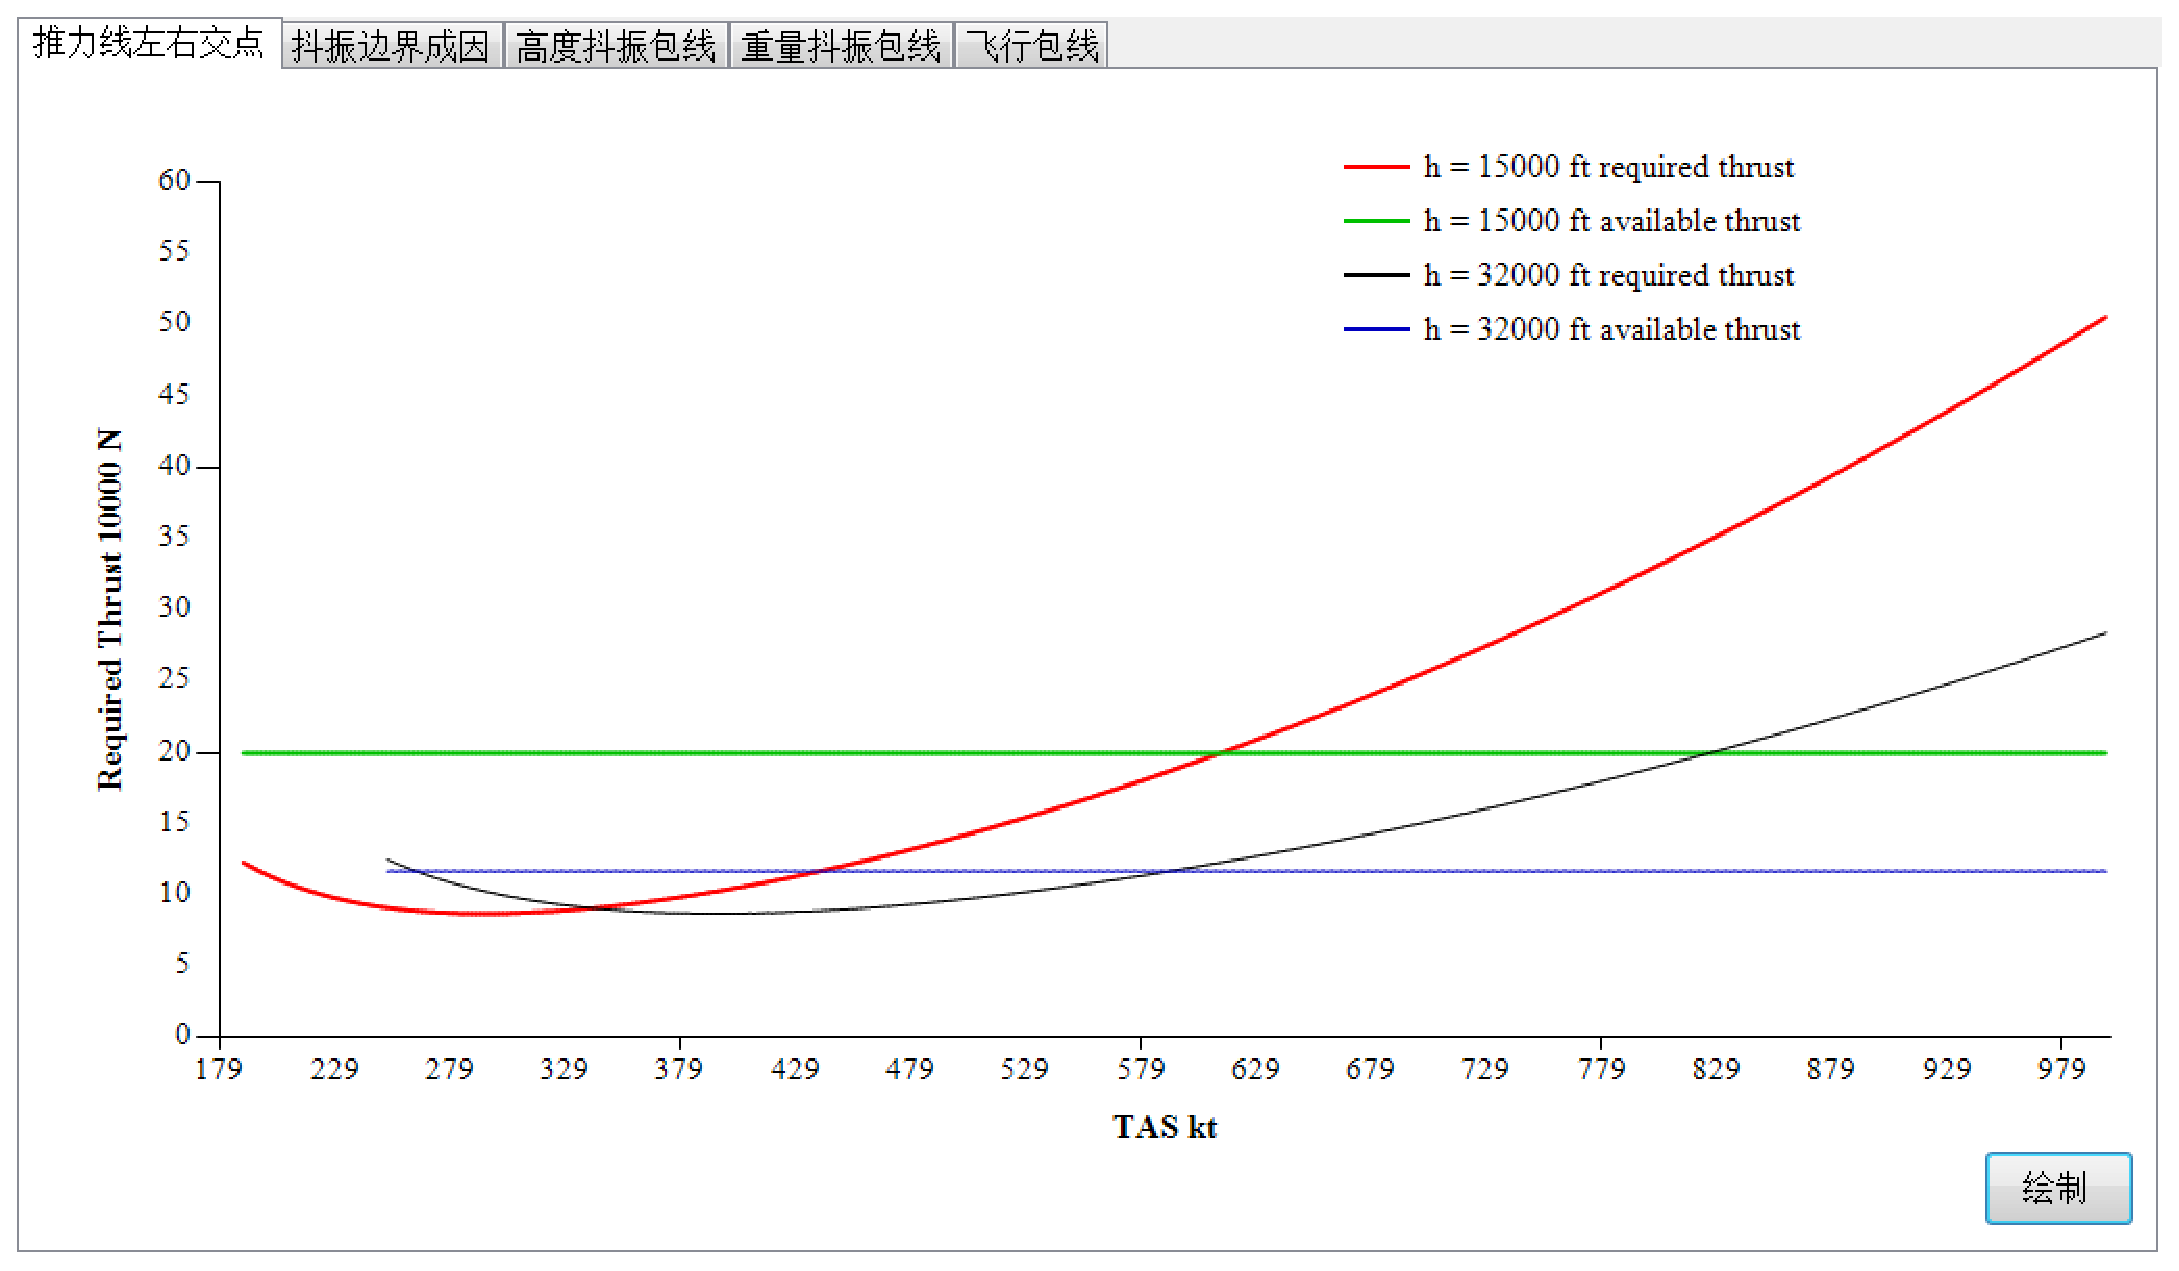
\includegraphics[width=0.8\textwidth]{pic/leftrightcrosspointinF-V.eps}\hspace{30pt}
	\caption{空客300-600推力线左右交点}\label{leftrightcrosspointinF-V}
\end{figure}


(2)抖振边界成因

抖振边界实际上是由升力系数曲线和抖振升力系数曲线的左右交点形成的。根据式\ref{CL-M}绘制$C_{\rm L}$\ - $M$曲线,选取波音737-800运行手册中提供的抖振升力系数,令折减系数$factor=0.98$,绘制$C_{\rm L,buffet}$\ -\ $M$曲线。这两条曲线的左右交点即为抖振边界对应的速度。随着高度升高或航空器重量增大,升力系数曲线向右移动,导致左右交点均向内移,飞机受抖振限制能飞的速度区间变小。

绘制空客300-600飞机在15000 $\rm ft$与在30000 $\rm ft$上的$C_{\rm L}$\ - $M$和$C_{\rm L,buffet}$\ -\ $M$曲线。如图\ref{buffetboundary}所示,可以看到高度升高,抖振边界范围缩小。

\begin{figure}[h]
	\centering
	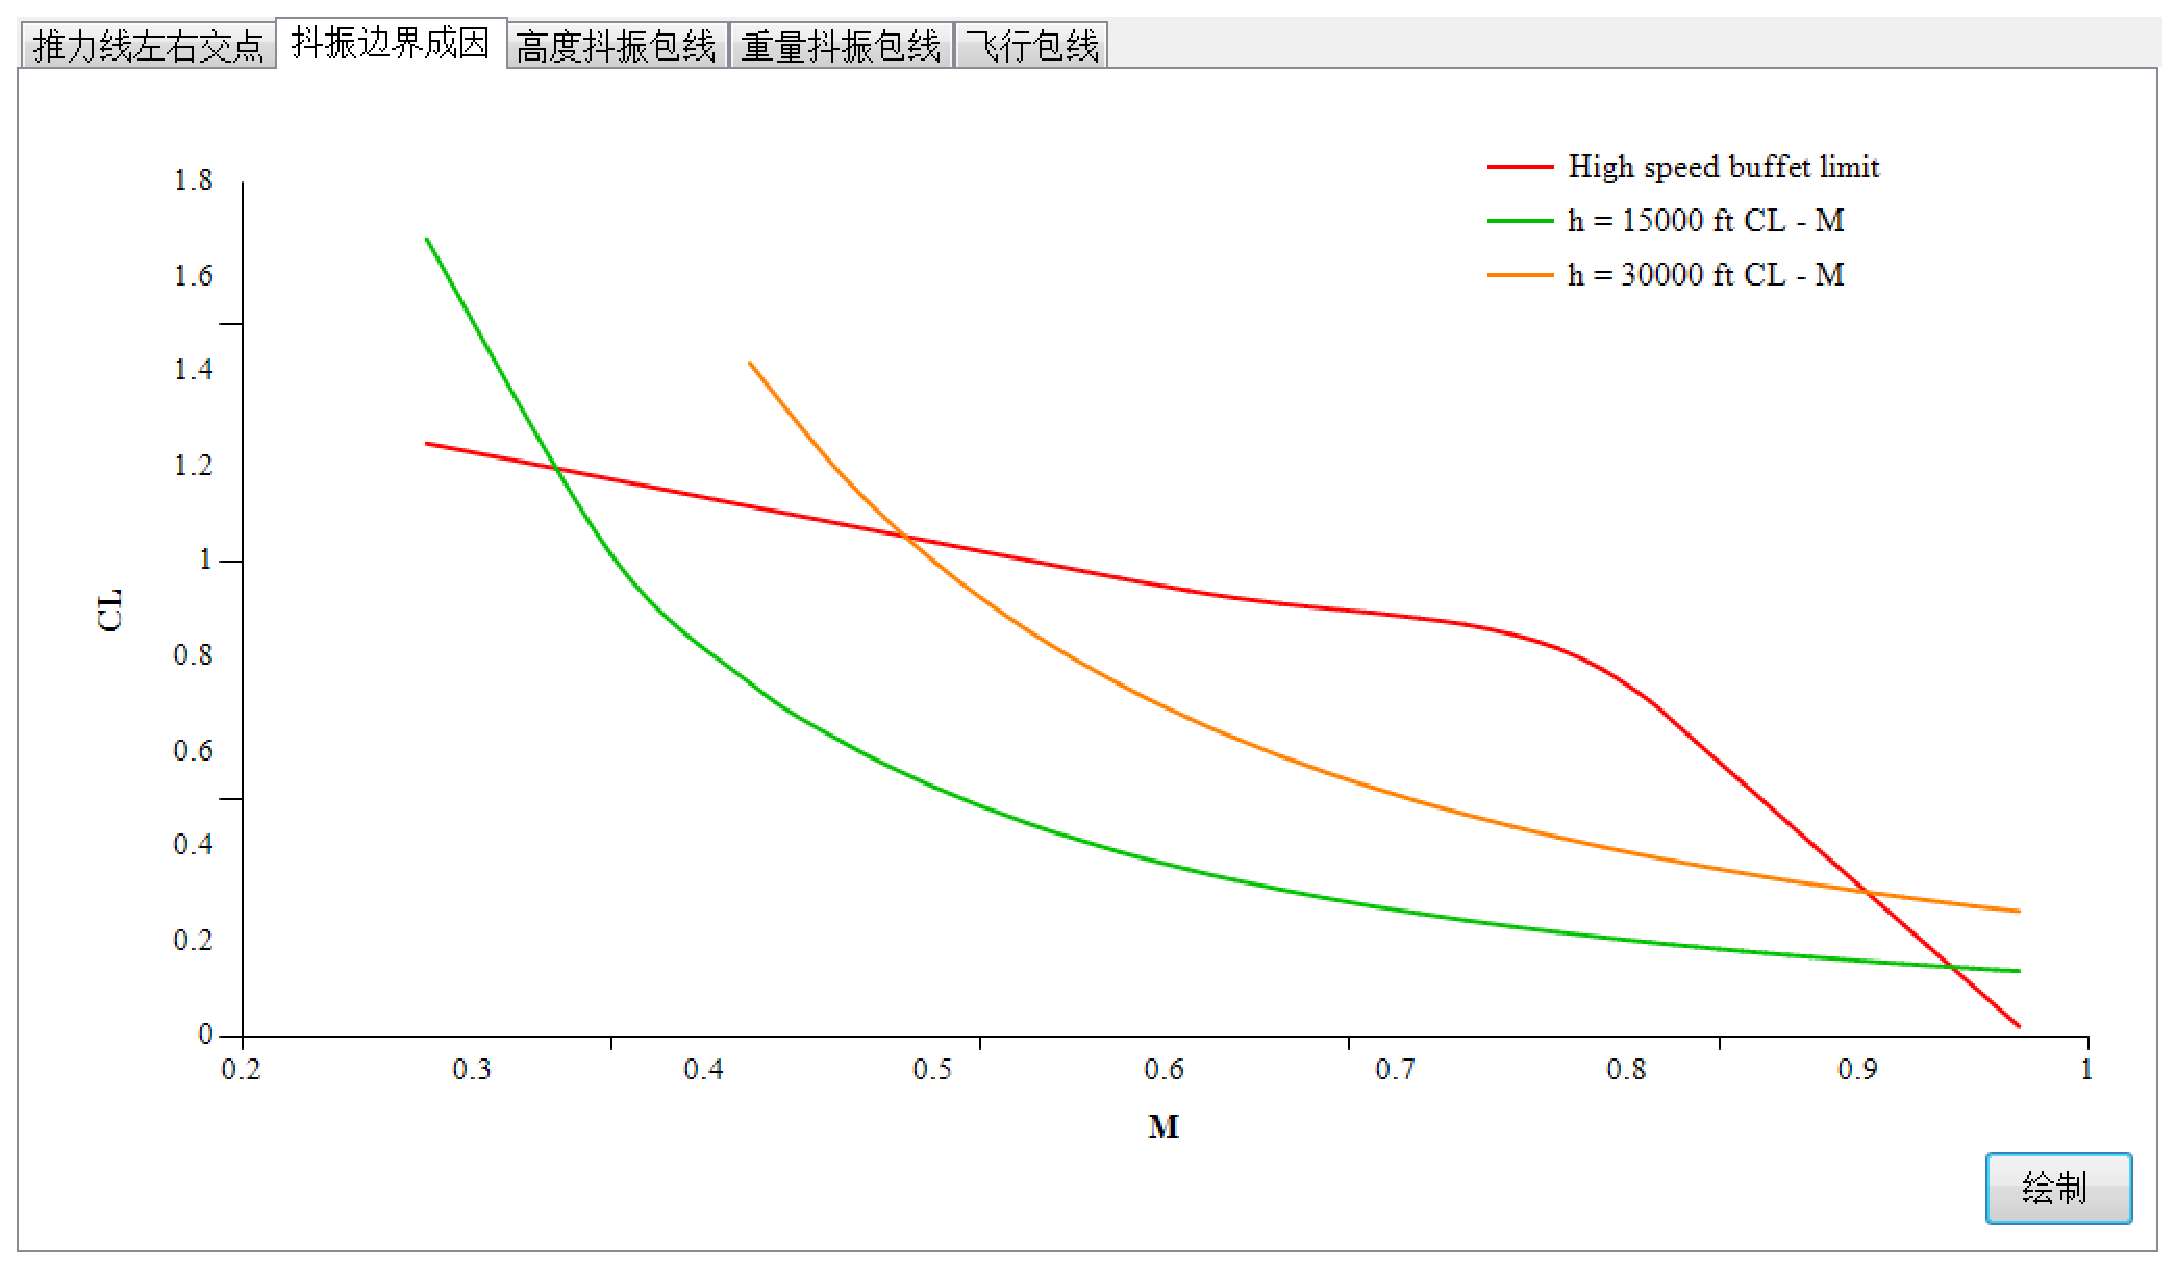
\includegraphics[width=0.8\textwidth]{pic/buffetboundary.eps}\hspace{30pt}
	\caption{空客300-600抖振边界}\label{buffetboundary}
\end{figure}



(3)高度抖振包线

根据抖振边界的成因,将每个高度上的抖振边界速度在$h$\ -\ $M$图中标出,连接这些点绘制高度抖振包线。包线的左侧为低速抖振边界线,右侧为高速抖振边界,顶点对应的高度为升限。由于随着航空器重量增大,能飞的抖振速度范围变小,故增大重量会使包线向里收缩。

绘制空客300-600飞机在不同重量下的高度抖振包线。如图\ref{buffetlimitwithh}所示,可以看到随重量增大,包线內移。每条包线的顶点即为飞机在该重量下的升限。

\begin{figure}[h]
	\centering
	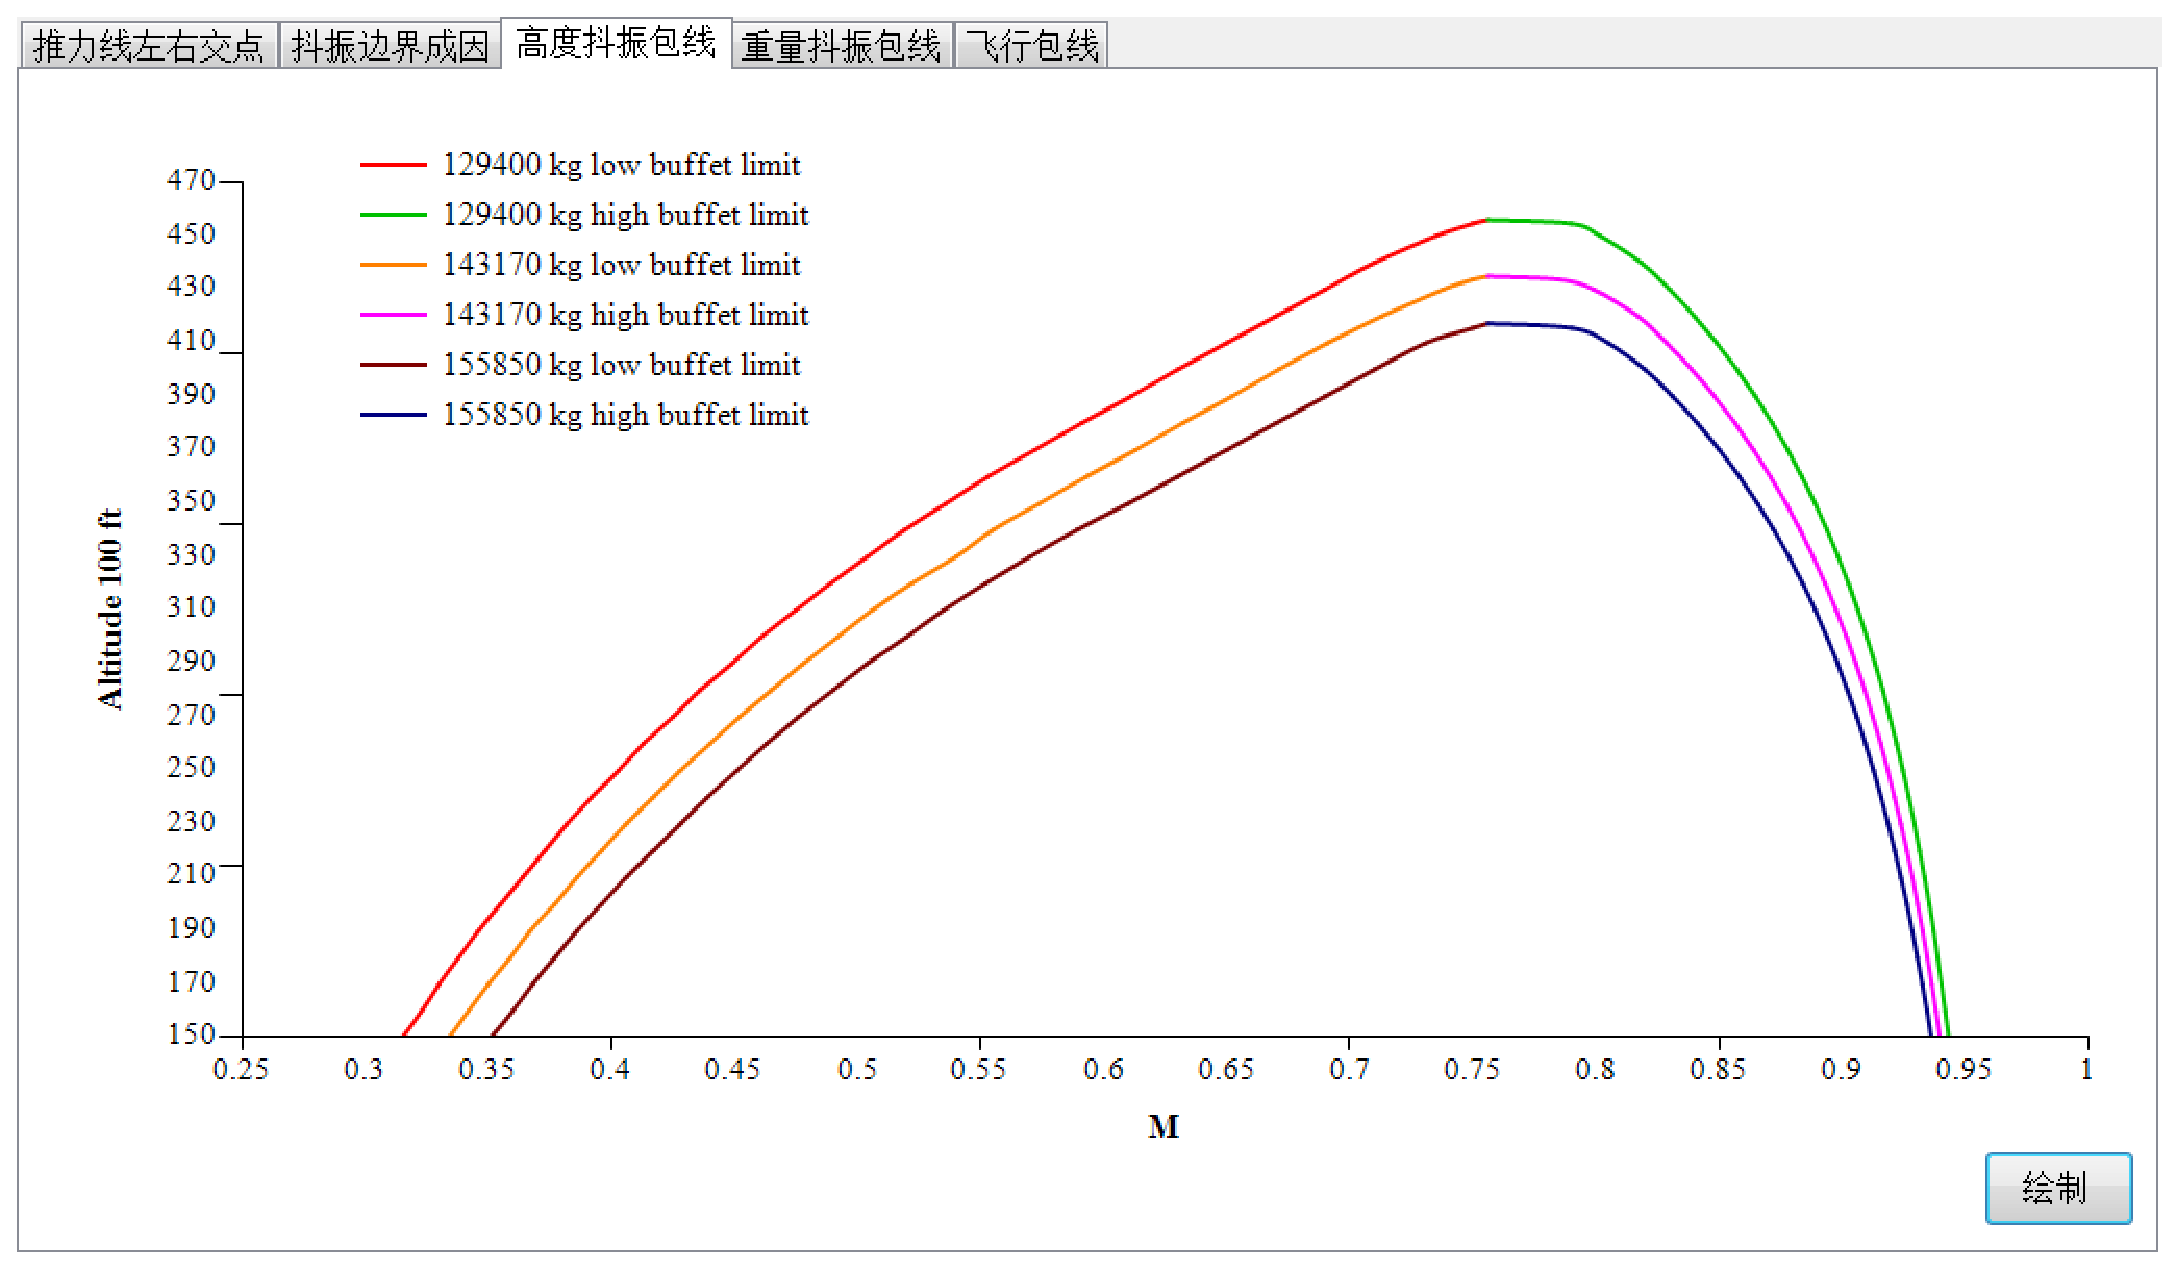
\includegraphics[width=0.8\textwidth]{pic/buffetlimitwithh.eps}\hspace{30pt}
	\caption{空客300-600高度抖振包线}\label{buffetlimitwithh}
\end{figure}



(4)重量抖振包线(Buffet Onset)

将航空器在每个重量下的抖振边界速度在$W$\ -\ $M$图中标出,连接成重量抖振包线。同样地,高度升高造成包线向内收缩。

绘制空客300-600飞机在FL330、FL350及FL370的高度抖振包线,并在图中标注飞机的最大飞行马赫数$M_{\rm MO}$,如图\ref{buffetlimitwithWwithouttrim}所示。把高度抖振包线速度超过数$M_{\rm MO}$的部分剪切掉,就形成了运行手册中的抖振包线(Buffet Onset),如图\ref{buffetlimitwithWtrim}所示。

\begin{figure}[h]
	\centering
	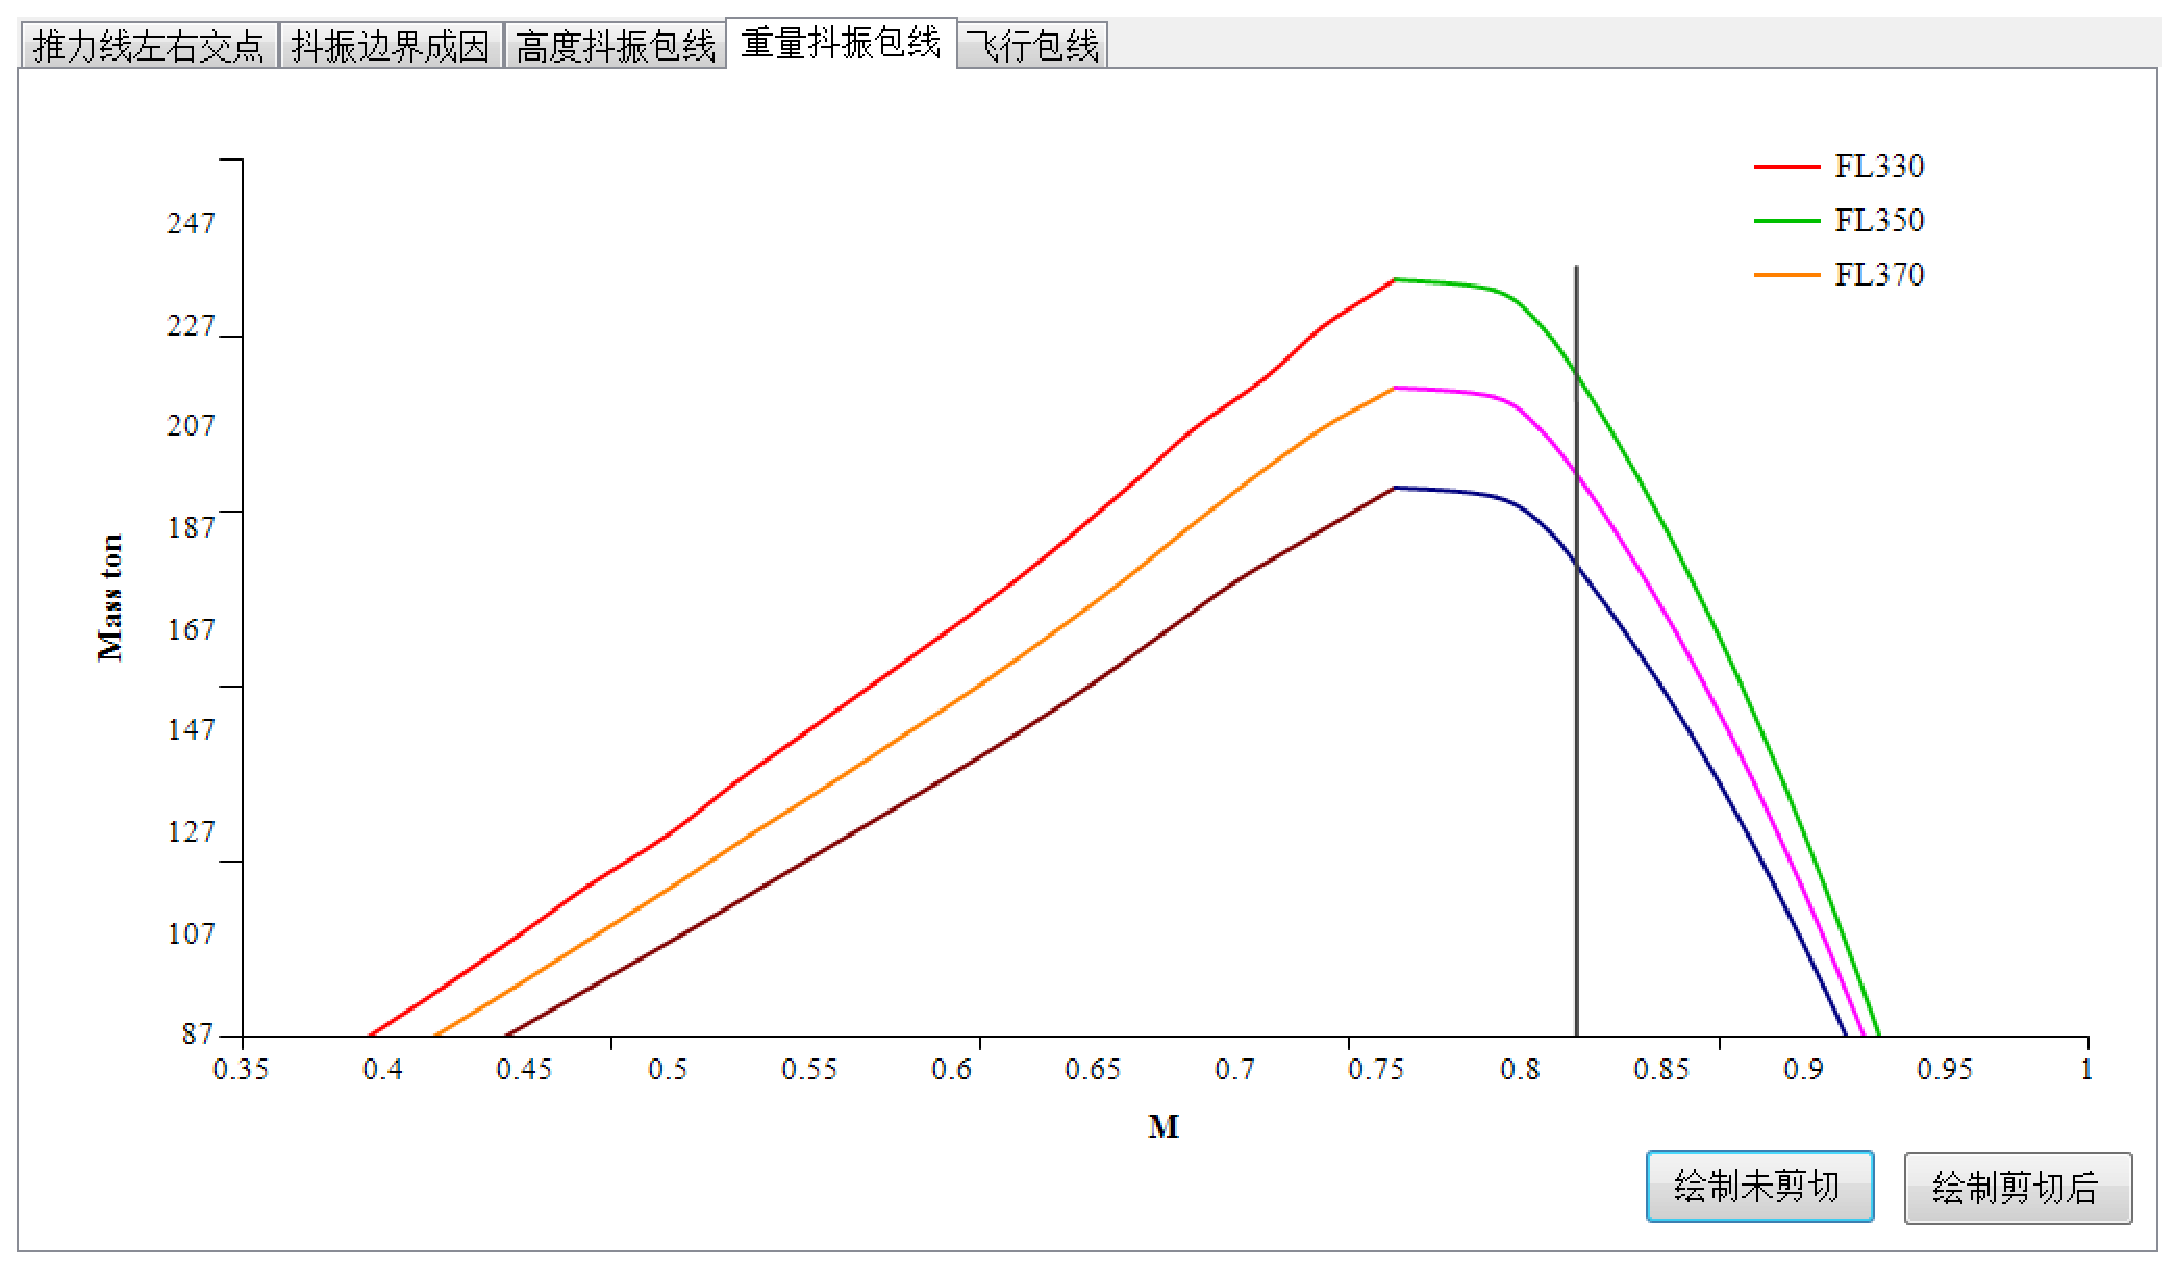
\includegraphics[width=0.8\textwidth]{pic/buffetlimitwithWwithouttrim.eps}\hspace{30pt}
	\caption{空客300-600重量抖振包线(未取交集)}\label{buffetlimitwithWwithouttrim}
\end{figure}

\begin{figure}[h]
	\centering
	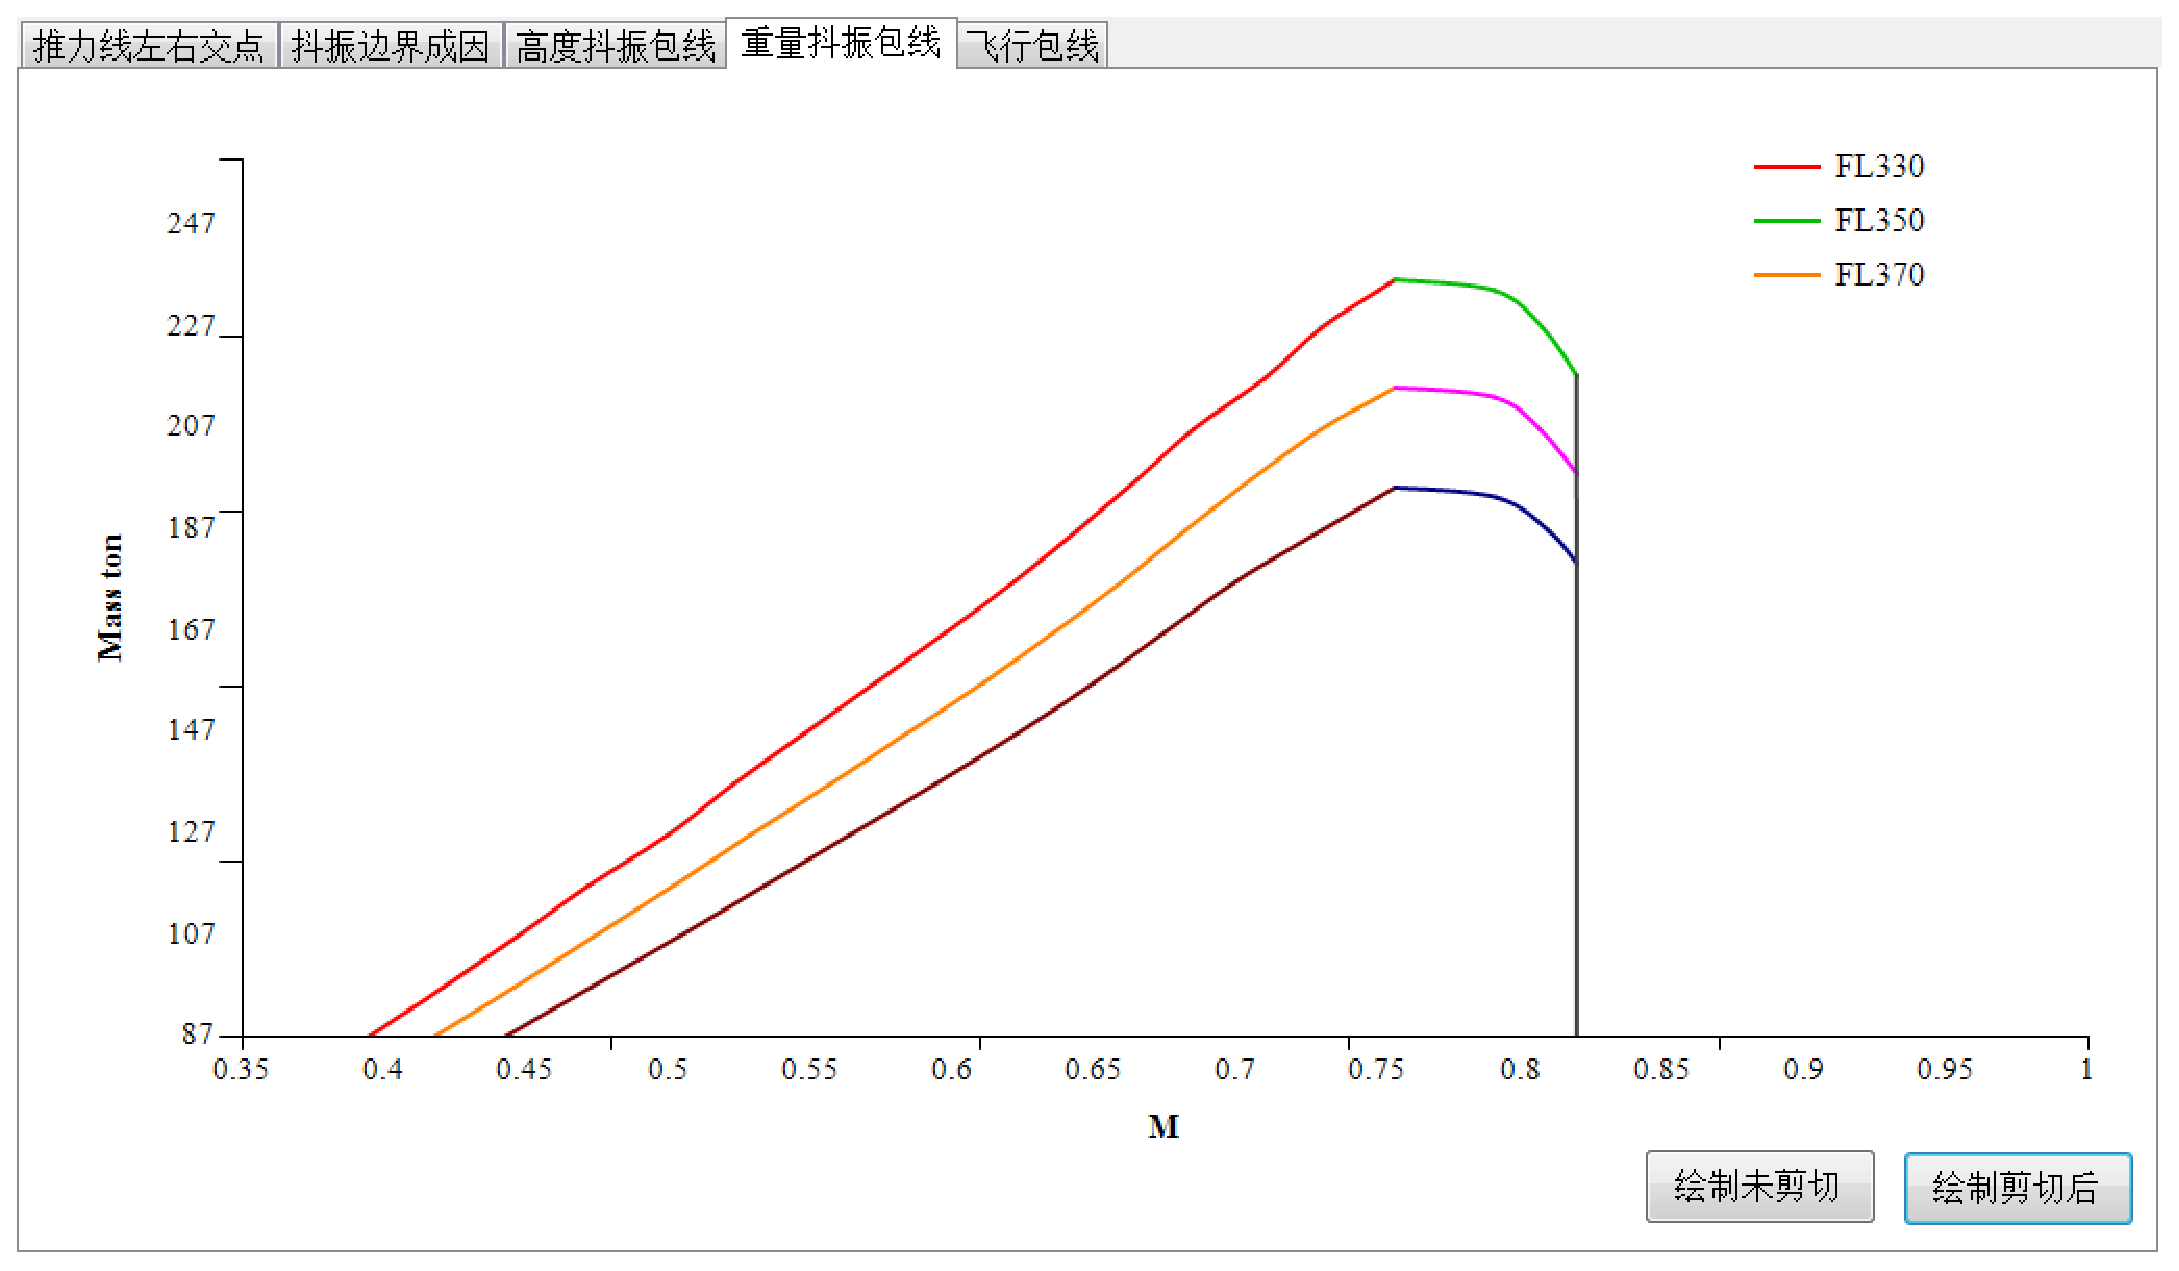
\includegraphics[width=0.8\textwidth]{pic/buffetlimitwithWtrim.eps}\hspace{30pt}
	\caption{空客300-600重量抖振包线(取交集)}\label{buffetlimitwithWtrim}
\end{figure}


(5)飞行包线

将航空器失速速度随高度、所需推力和可用推力曲线左交点随高度曲线、低速抖振边界随高度、$V_{\rm MO}$随高度、$M_{\rm MO}$随高度、所需推力和可用推力曲线右交点随高度、高速抖振边界随高度这7条曲线在$h$\ -\ $v_{\rm TAS}$图中画出,取包线间的交集(公共部分)即可得到最终的飞行包线。空客300-600飞机的飞行包线如图\ref{flightenvelopewithouttrim}、\ref{flightenvelopetrim}所示。

\begin{figure}[H]
	\centering
	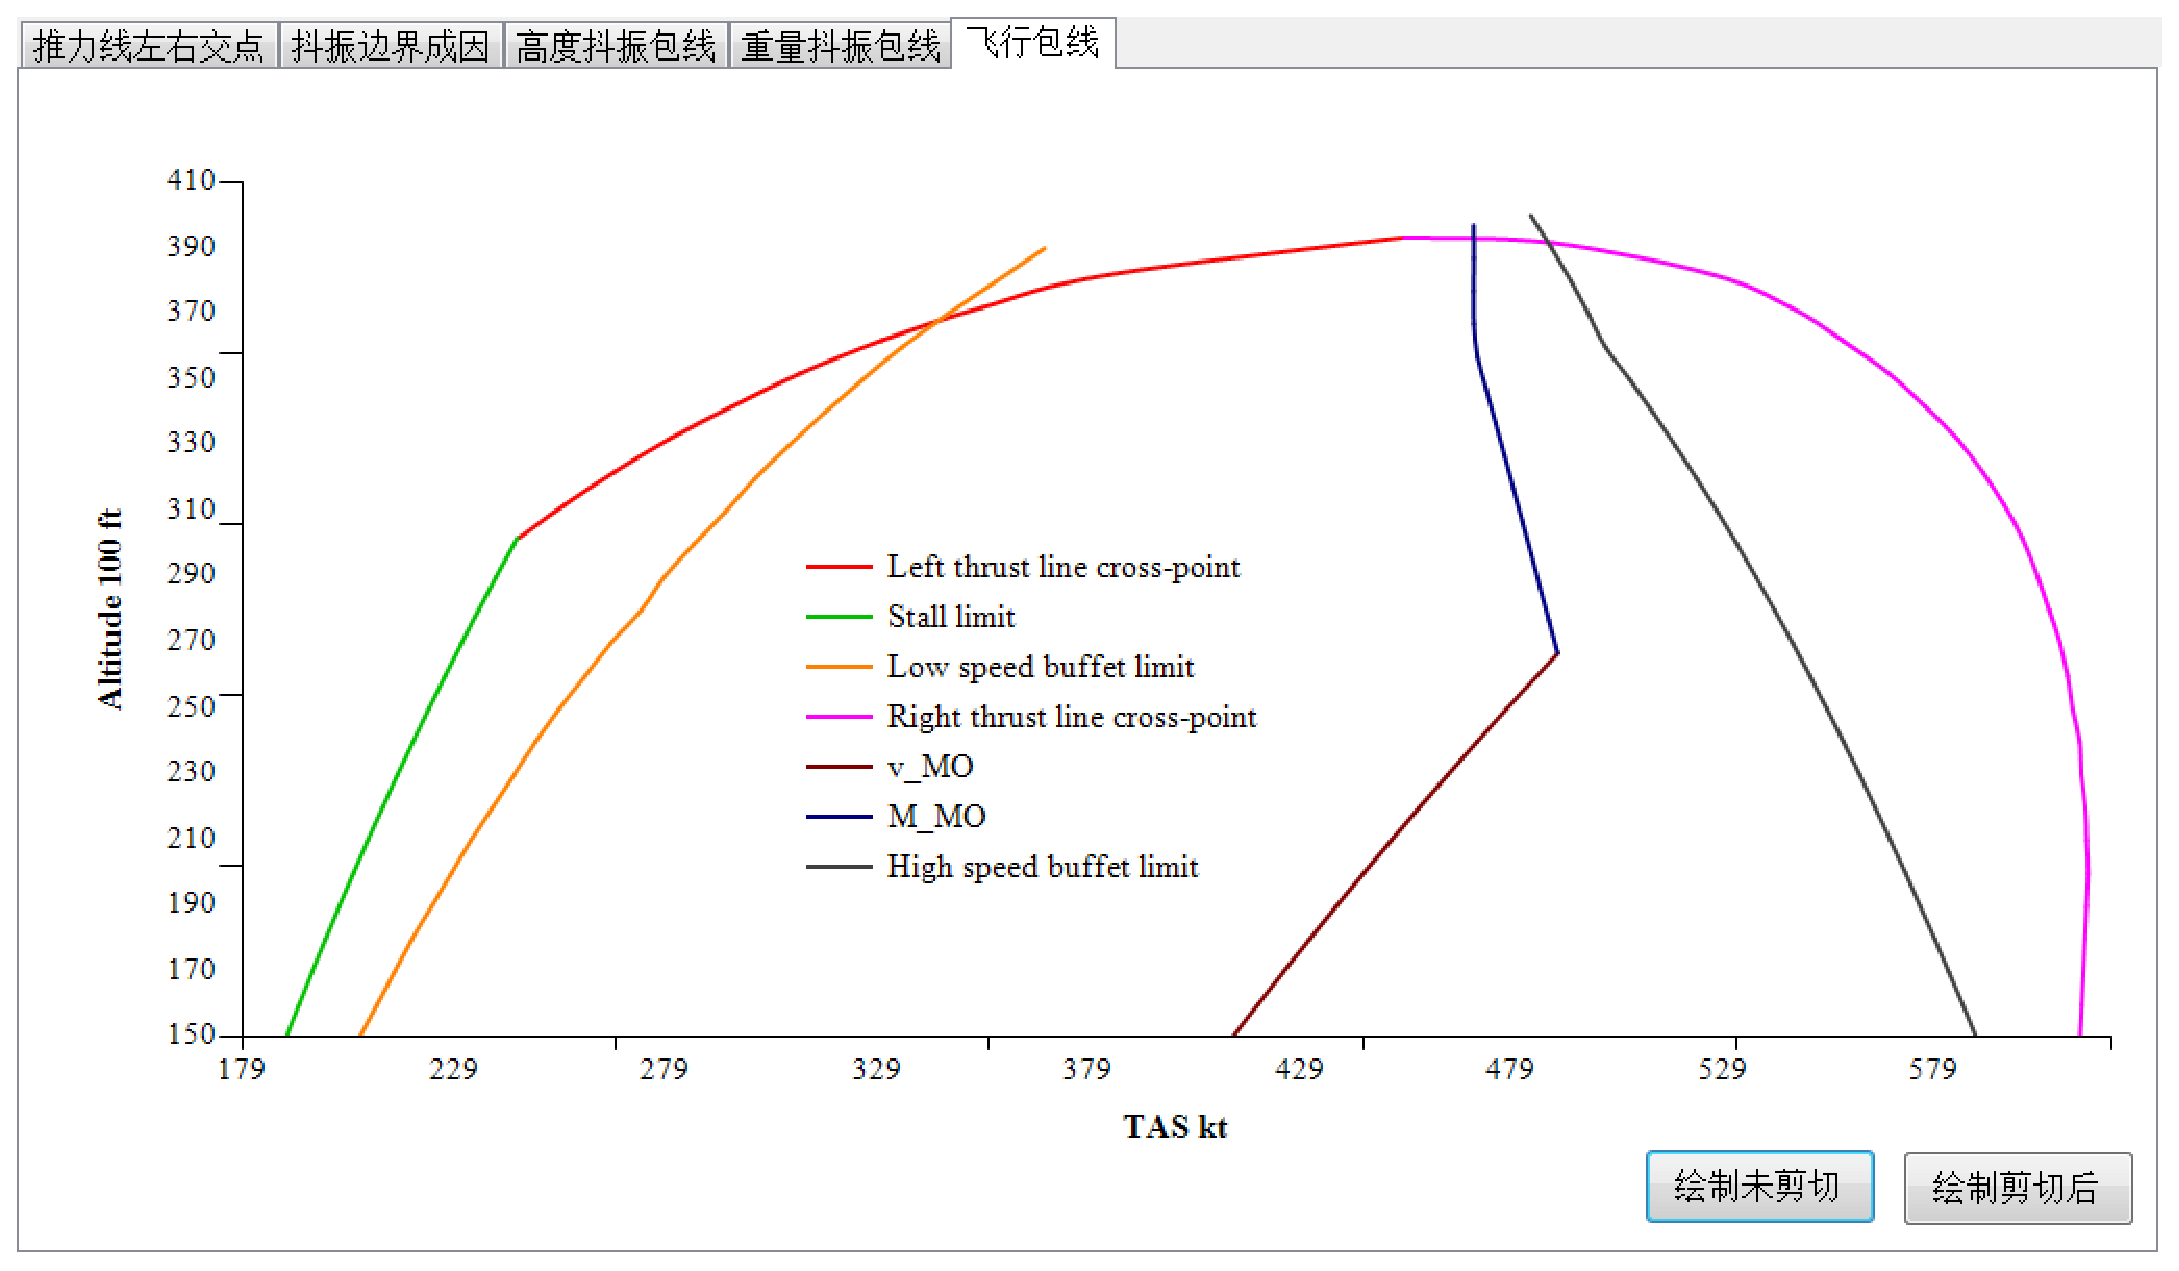
\includegraphics[width=0.8\textwidth]{pic/flightenvelopewithouttrim.eps}\hspace{30pt}
	\caption{空客300-600飞行包线(未取交集)}\label{flightenvelopewithouttrim}
\end{figure}

\begin{figure}[H]
	\centering
	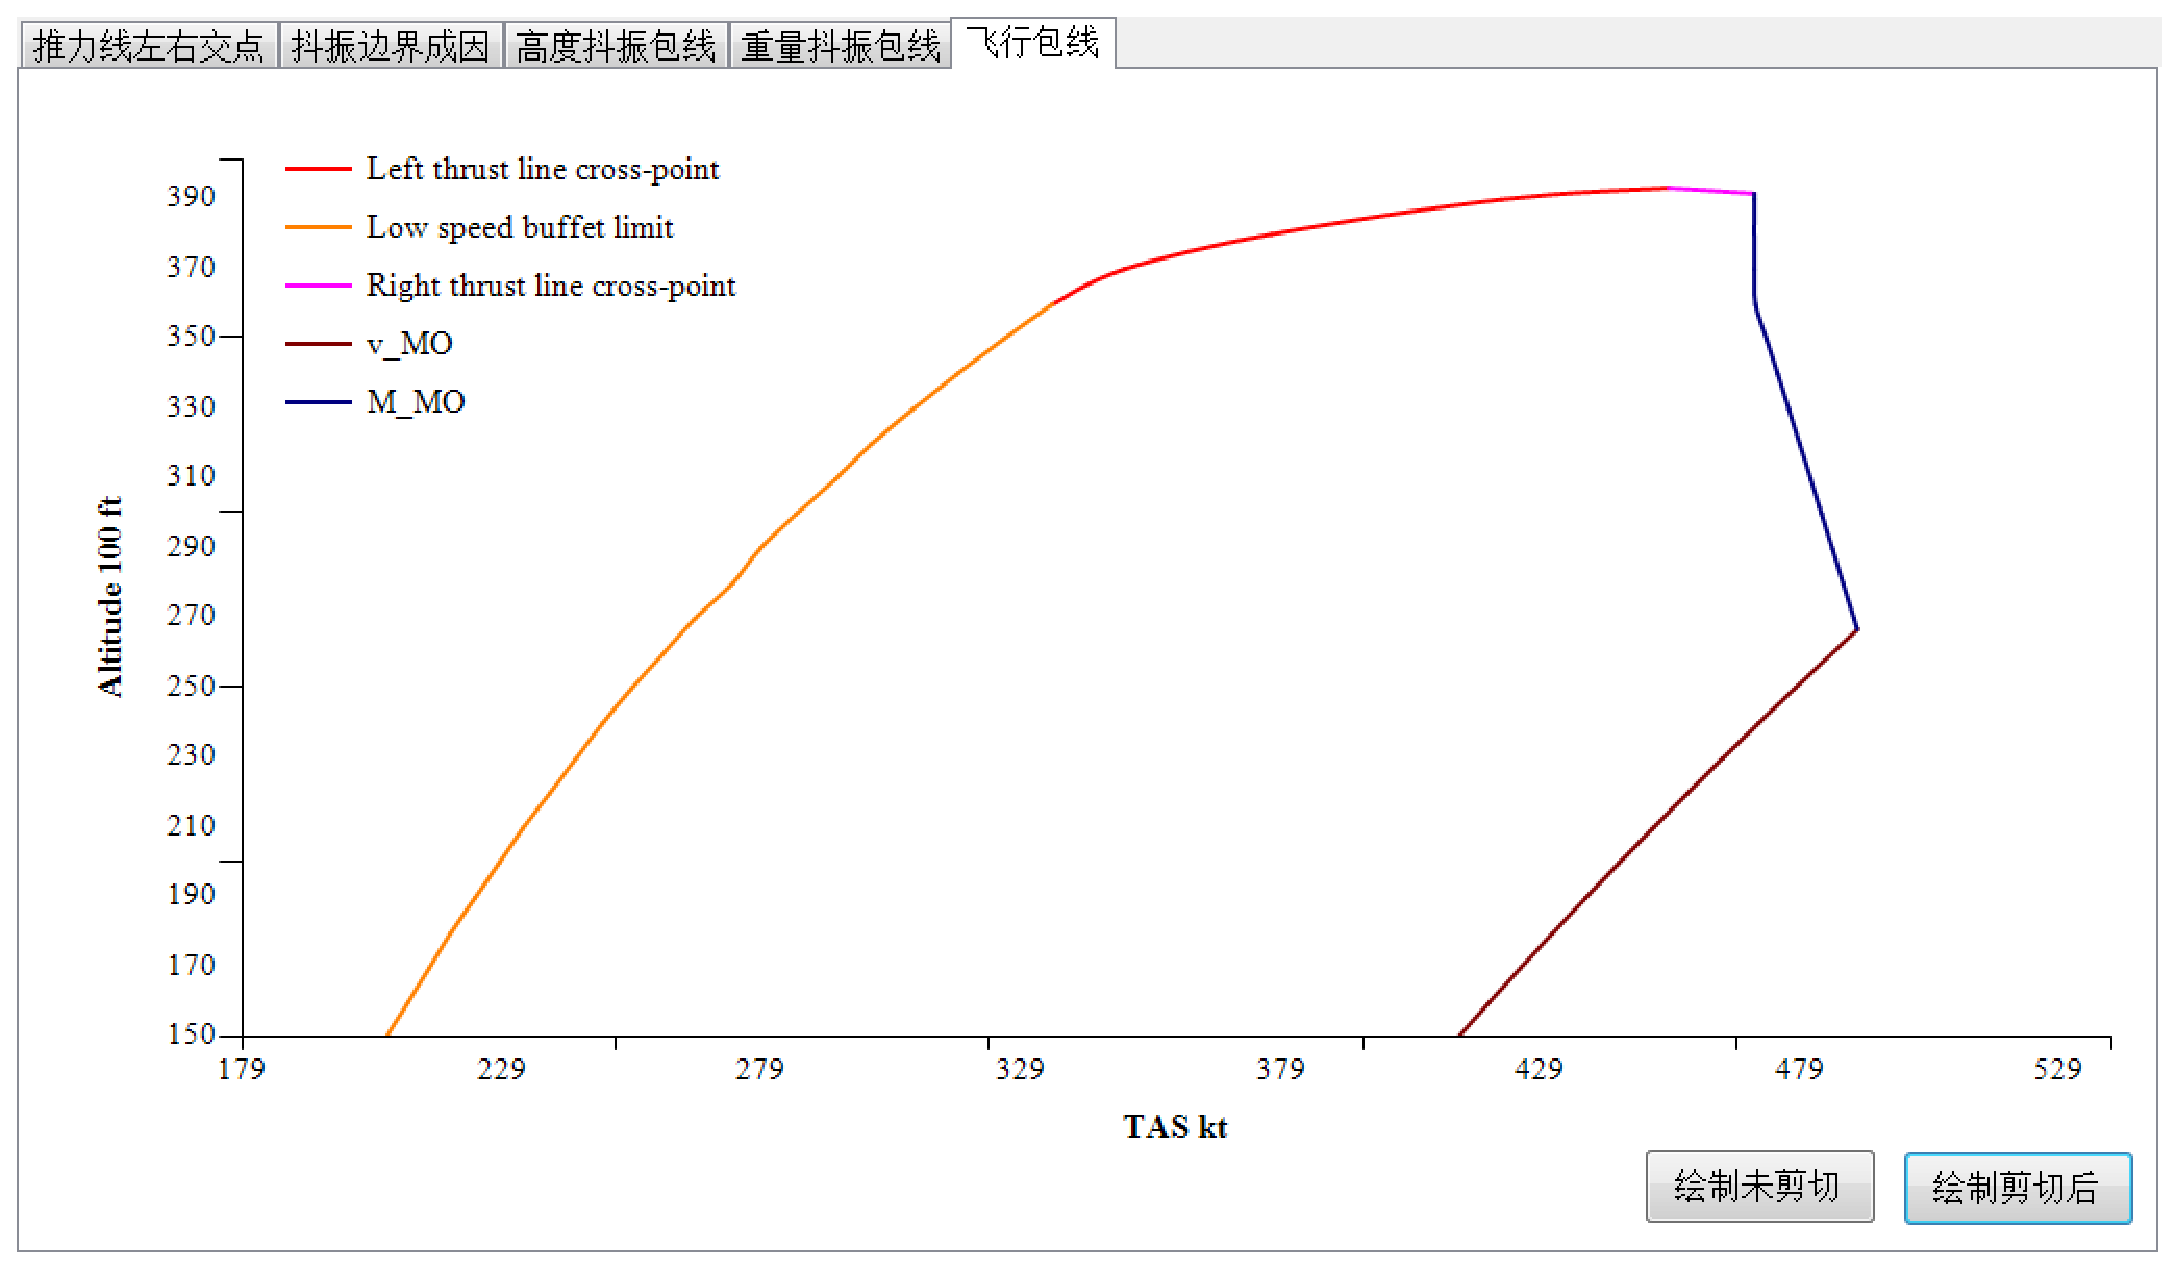
\includegraphics[width=0.8\textwidth]{pic/flightenvelopetrim.eps}\hspace{30pt}
	\caption{空客300-600飞行包线(取交集)}\label{flightenvelopetrim}
\end{figure}


\subsection{起飞阶段}

将飞机的加速继续起飞距离随决断速度$v_{\rm 1}$的曲线和中断起飞距离随$v_{\rm 1}$的曲线在$s_{\rm TO}$\ -\ $v{\rm 1}$图中画出,曲线交点处的起飞距离即为平衡场长,对应的速度为平衡场长下的决断速度。

绘制空客300-600飞机在海拔为0\ $\rm m$机场的平衡场长图,如图\ref{balancedfieldlength}所示,可以看到加速继续起飞距离随$v_{\rm 1}$增大而减小,中断起飞距离则随$v_{\rm 1}$增大而增大。两条曲线交点确定的平衡场长为2395\ $\rm m$,对应的决断速度$v_{\rm 1}$为127 $\rm kt$。

\begin{figure}[h]
	\centering
	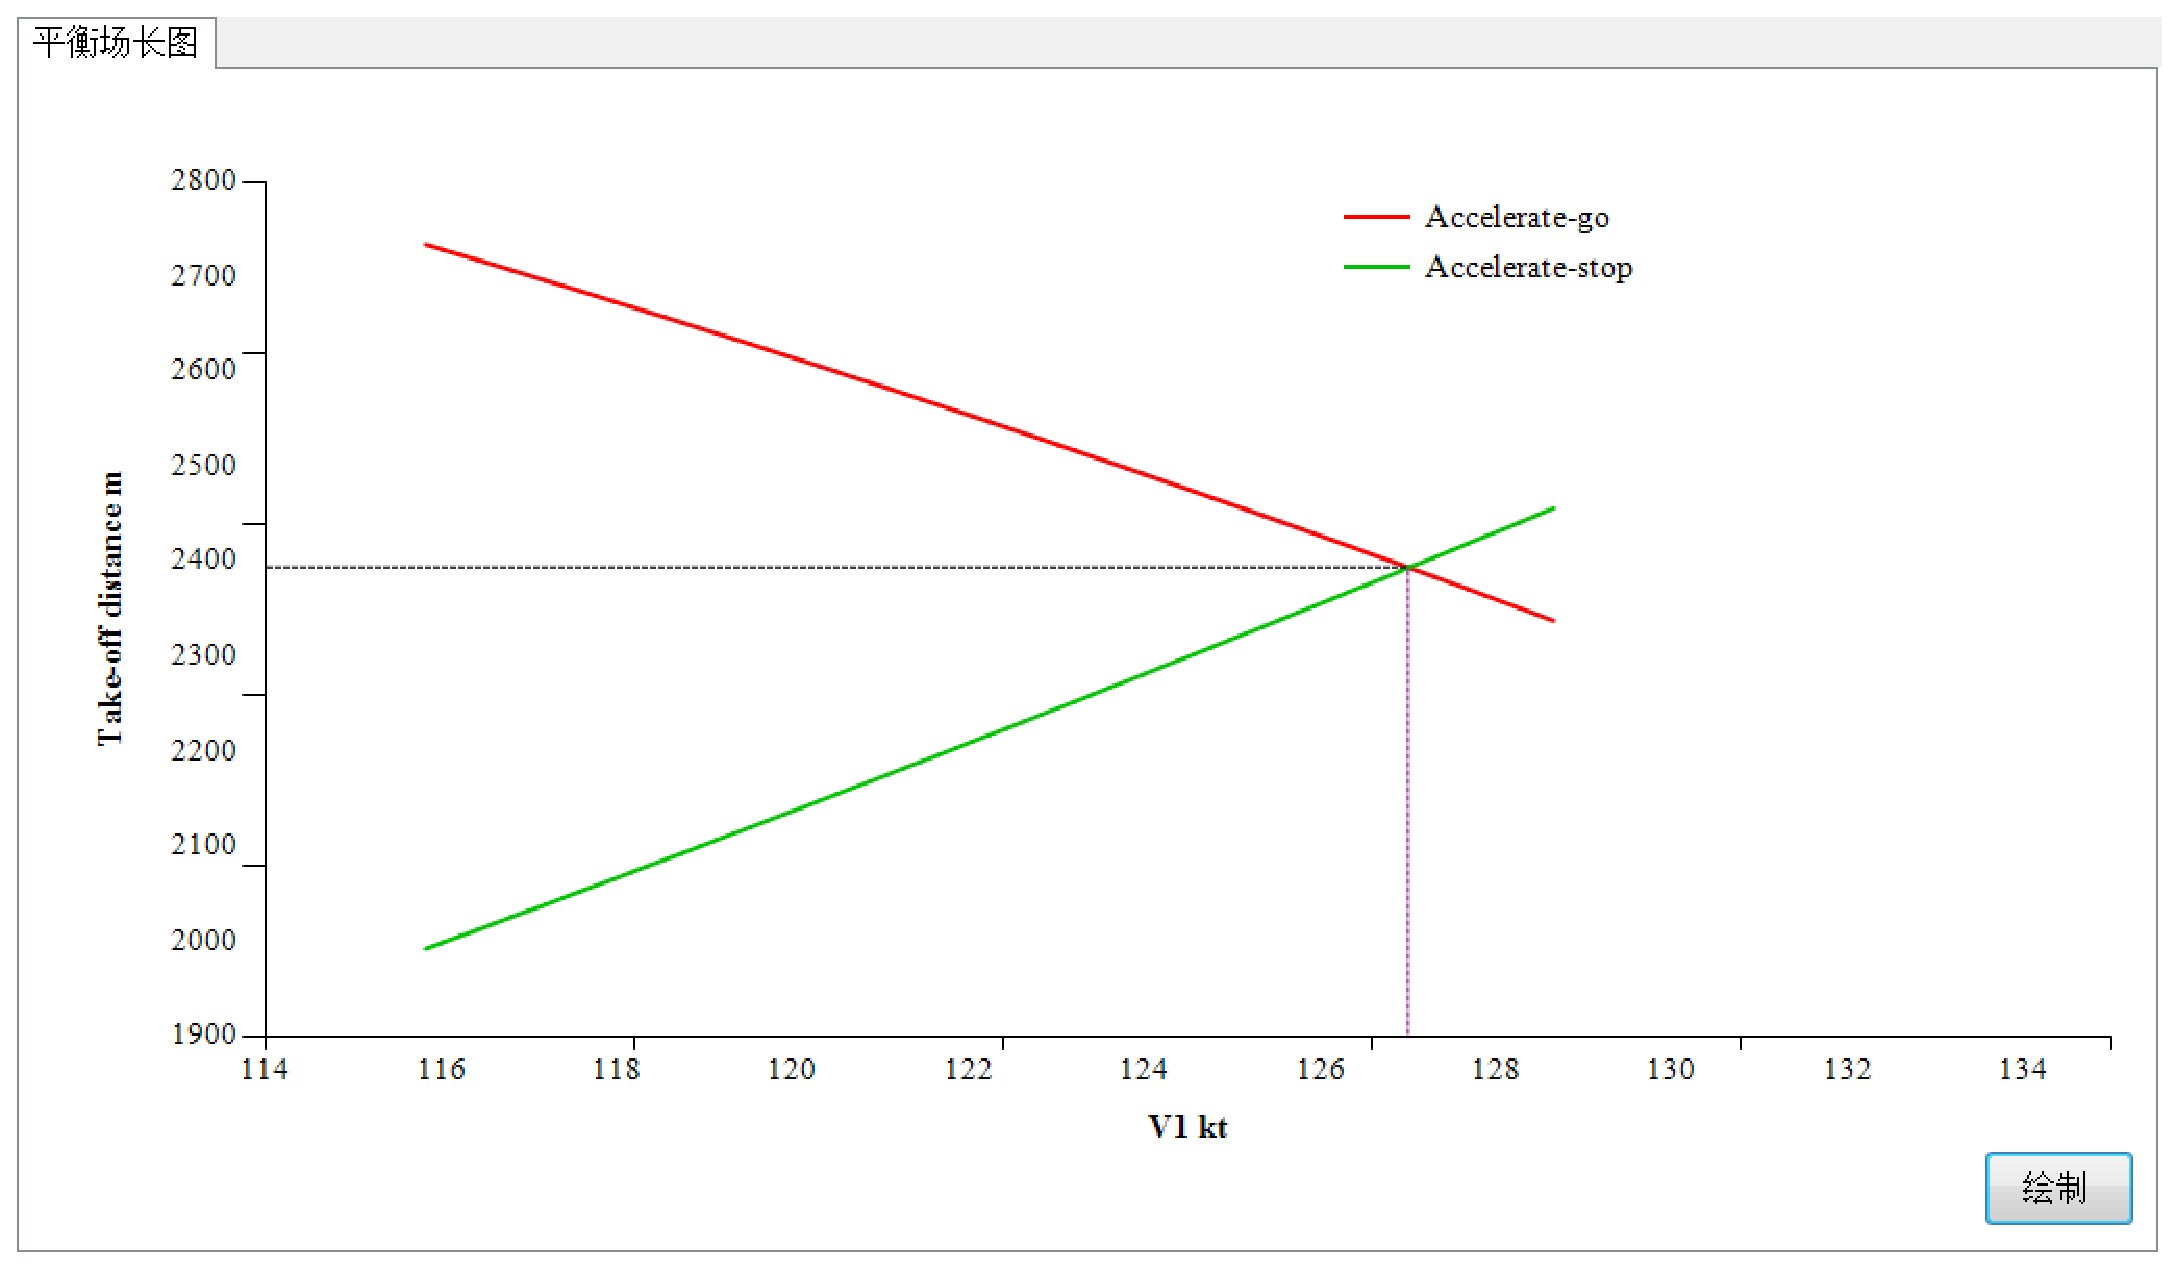
\includegraphics[width=0.8\textwidth]{pic/balancedfieldlength.eps}\hspace{30pt}
	\caption{空客300-600平衡场长图}\label{balancedfieldlength}
\end{figure}


\subsection{爬升阶段}

(1)爬升梯度随速度变化

由爬升率计算公式\ref{sintheta}可知,当航空器重量一定时,爬升梯度随剩余推力$F_{\rm redundant}$正向变化。根据剩余推力随速度的变化趋势,可知爬升梯度随速度增加的变化为先增大后减小。

绘制空客300-600飞机在18000\ $\rm ft$高度上爬升梯度随速度的变化曲线,如图\ref{cg}所示。

\begin{figure}[h]
	\centering
	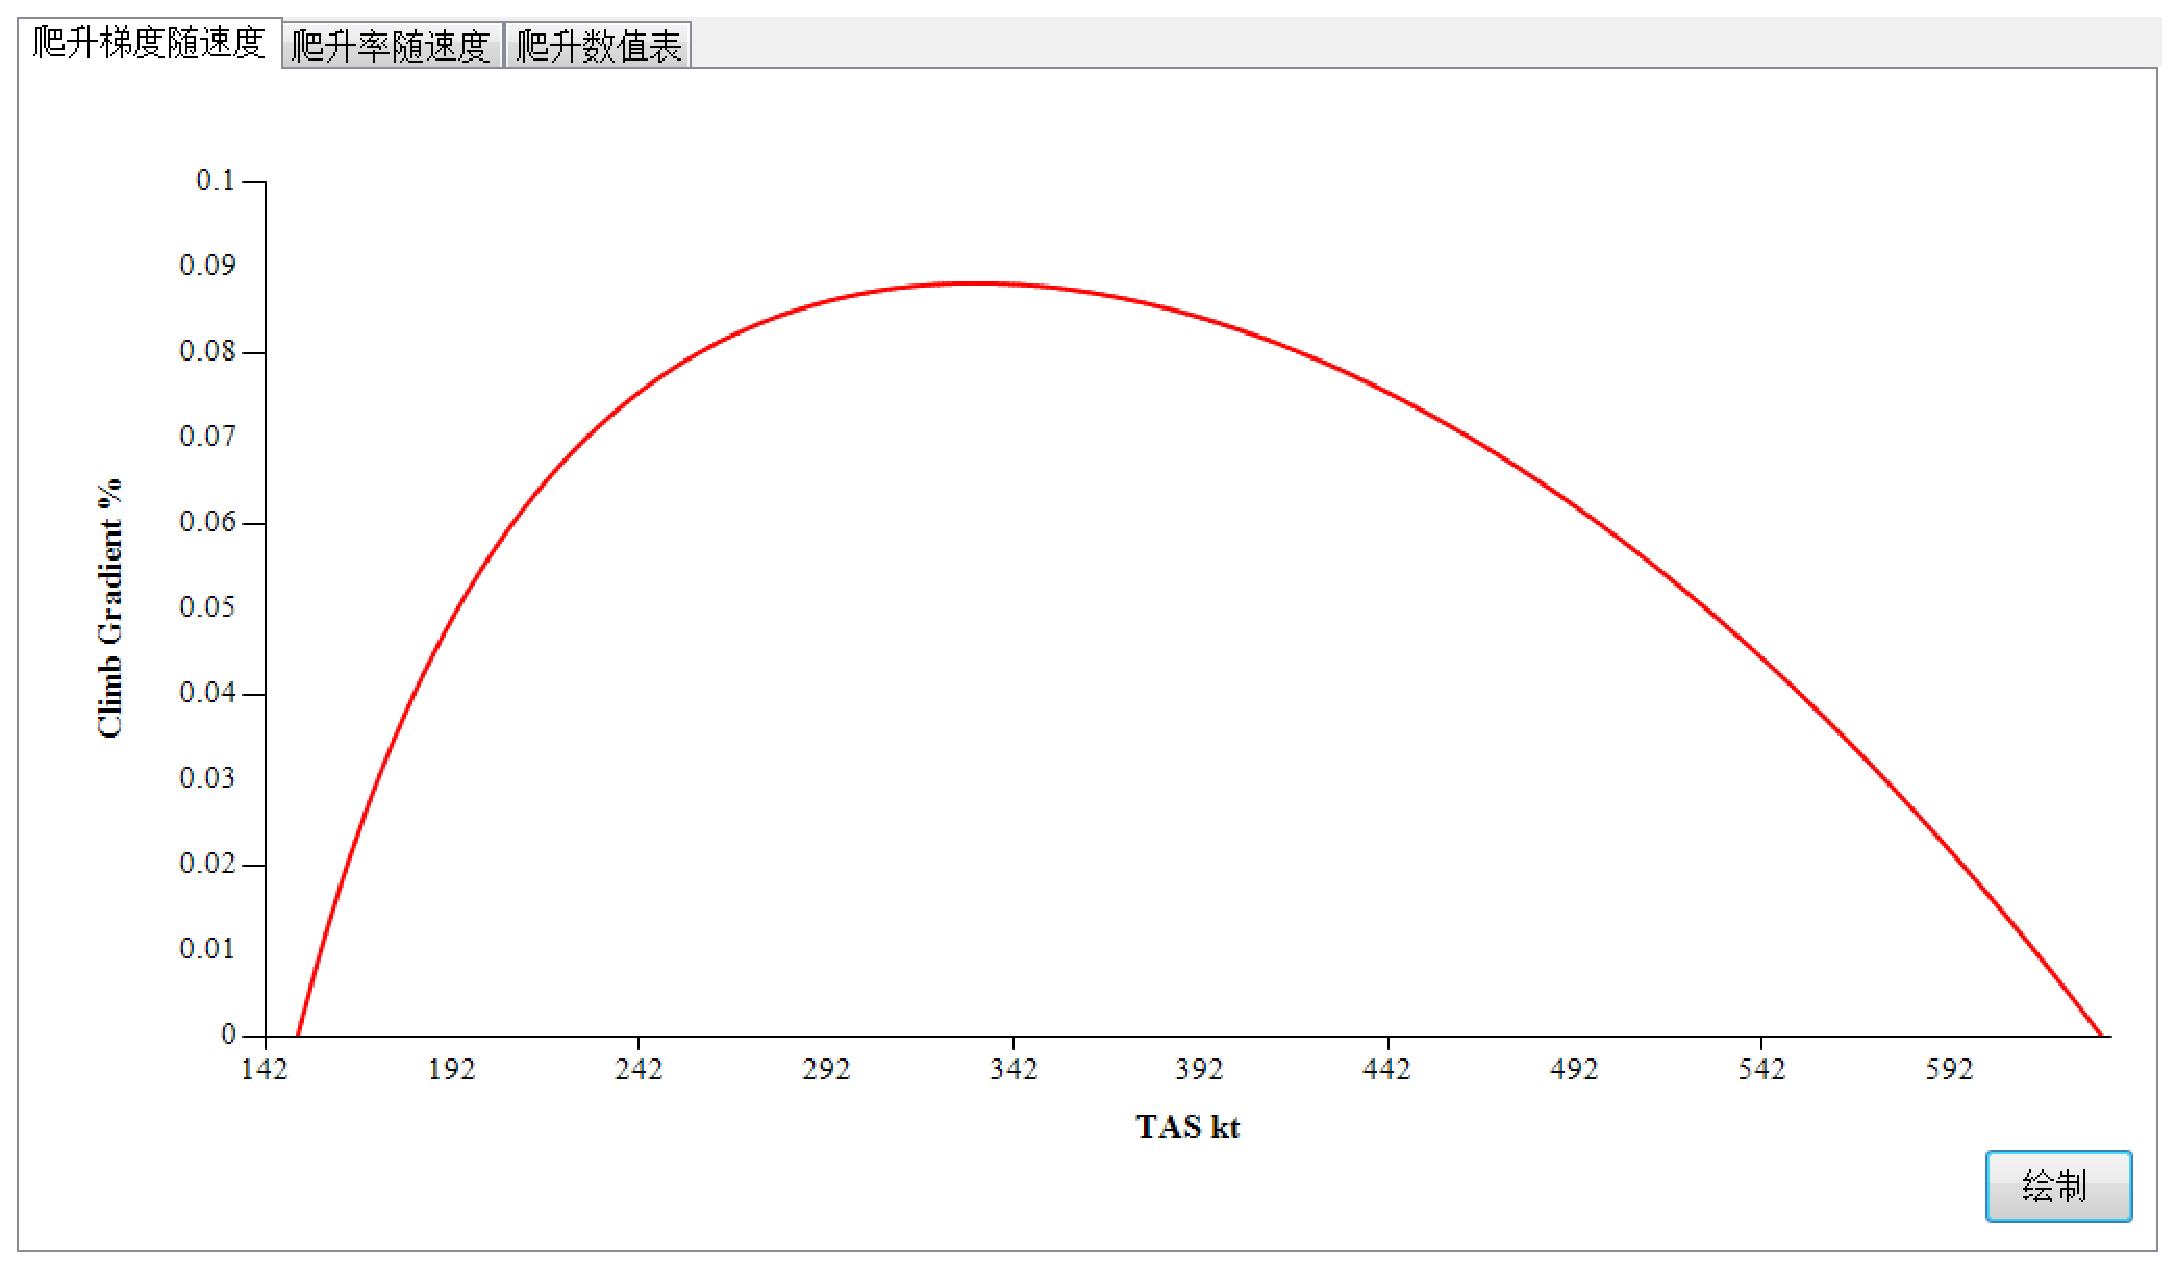
\includegraphics[width=0.8\textwidth]{pic/cg.eps}\hspace{30pt}
	\caption{空客300-600爬升梯度随速度曲线}\label{cg}
\end{figure}


(2)爬升率随速度

由式\ref{ROCD}及剩余功率随速度变化曲线可知,爬升率同样也随着速度增加先则增加后减小。

绘制空客300-600飞机在18000\ $\rm ft$高度上爬升率随速度的变化曲线,如图\ref{roc}所示。

\begin{figure}[h]
	\centering
	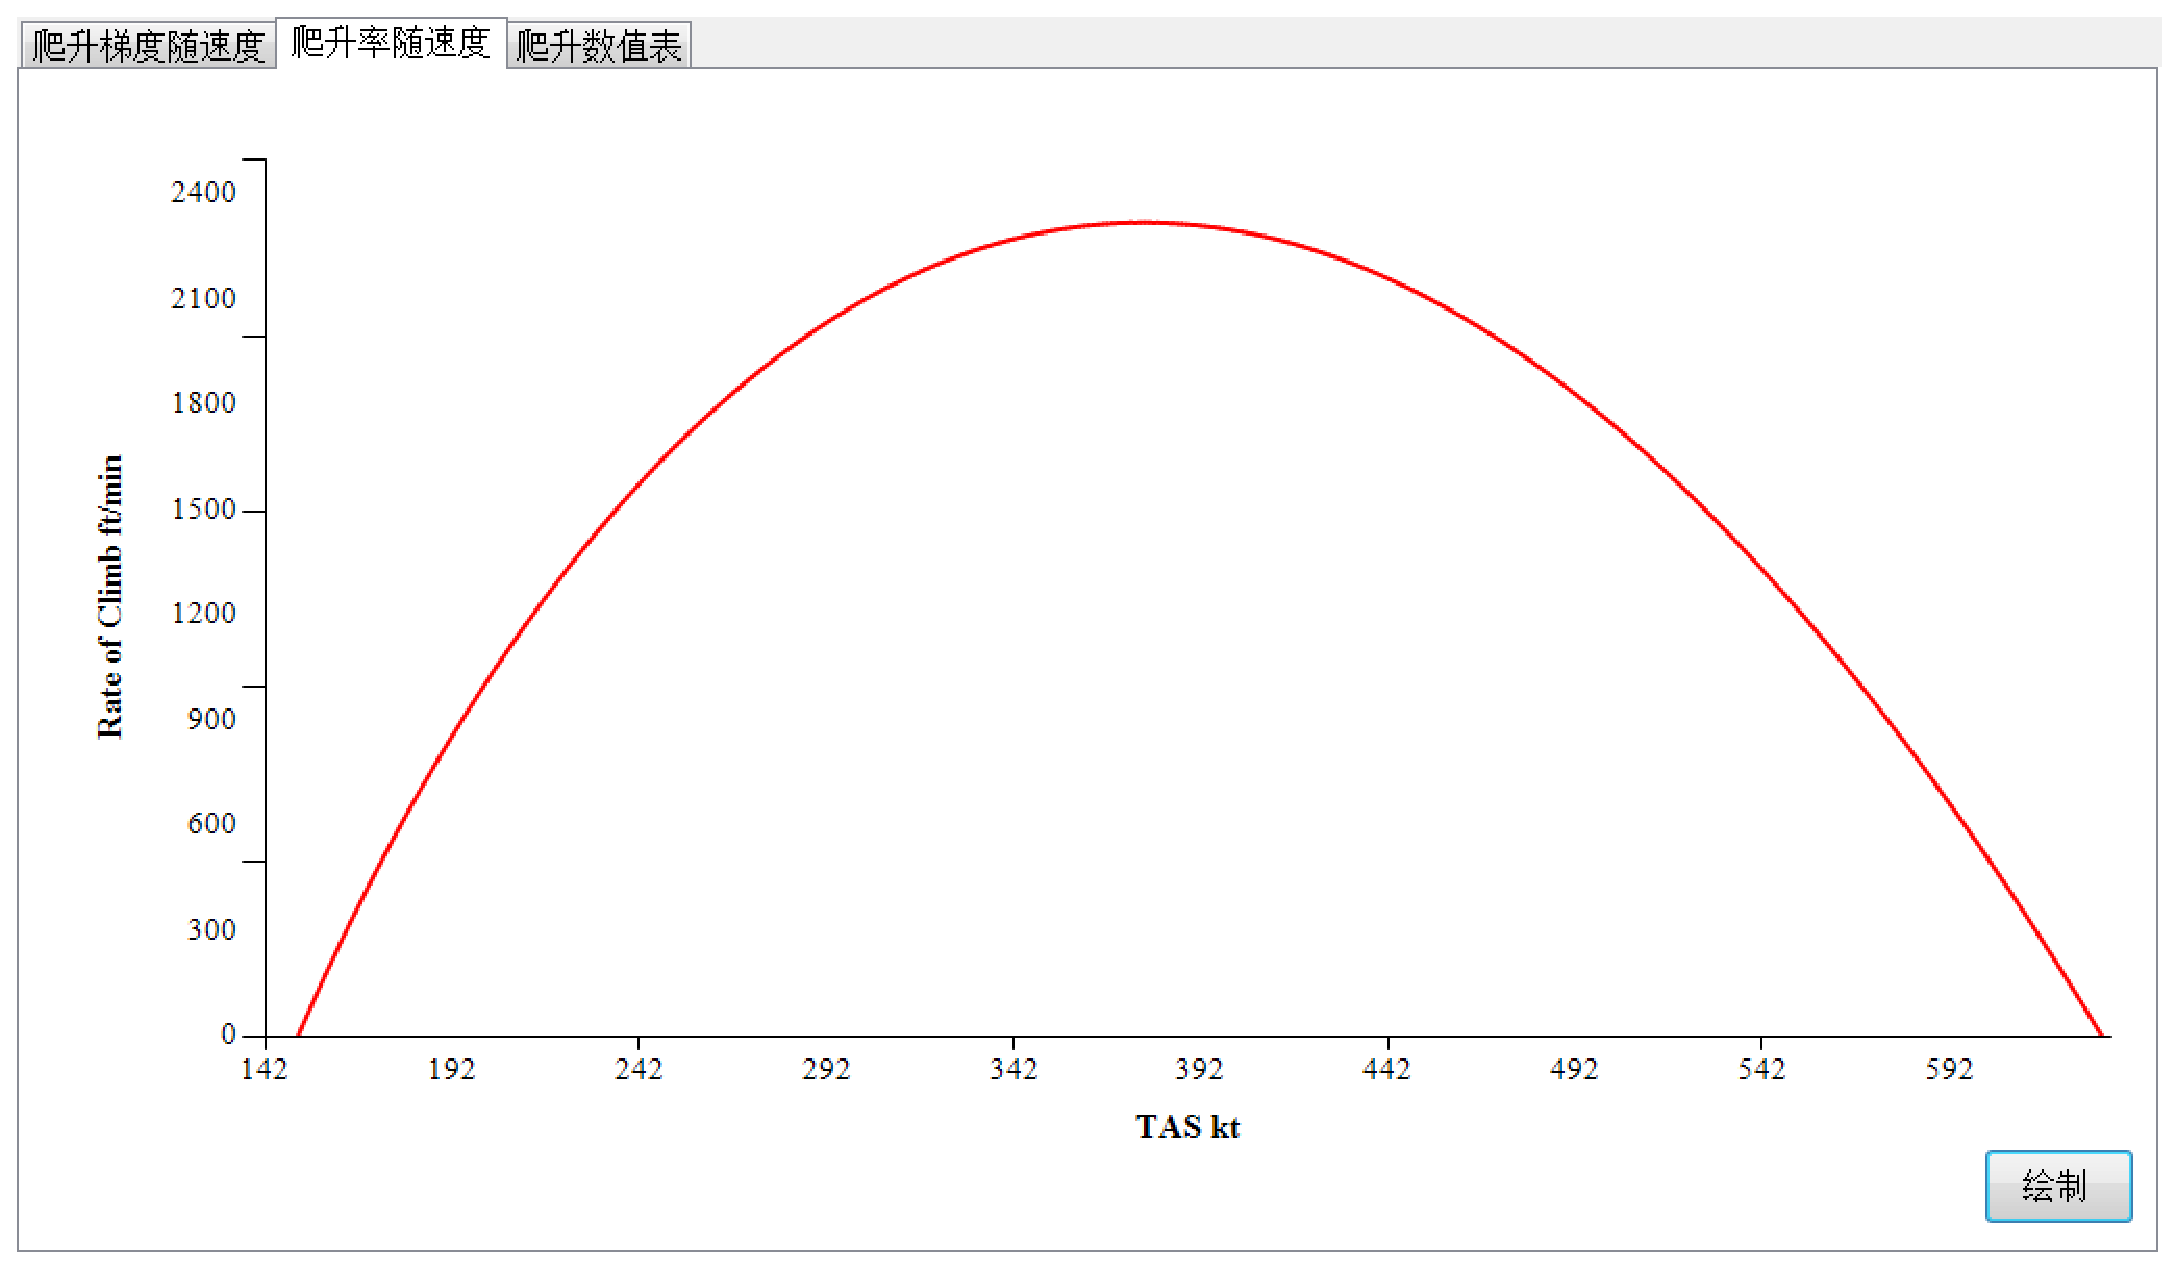
\includegraphics[width=0.8\textwidth]{pic/roc.eps}\hspace{30pt}
	\caption{空客300-600爬升率随速度曲线}\label{roc}
\end{figure}

(3)爬升数值表

调用Aircraft类中的计算函数,打印空客300-600飞机爬升阶段的数值表。如图\ref{climbtable}所示,表格展示了按等校正空速飞行,该机型飞机在各高度的真空速$v_{\rm TAS}$及不同重量下的爬升率$ROCD$和燃油流量$ff$。

\begin{figure}[h]
	\centering
	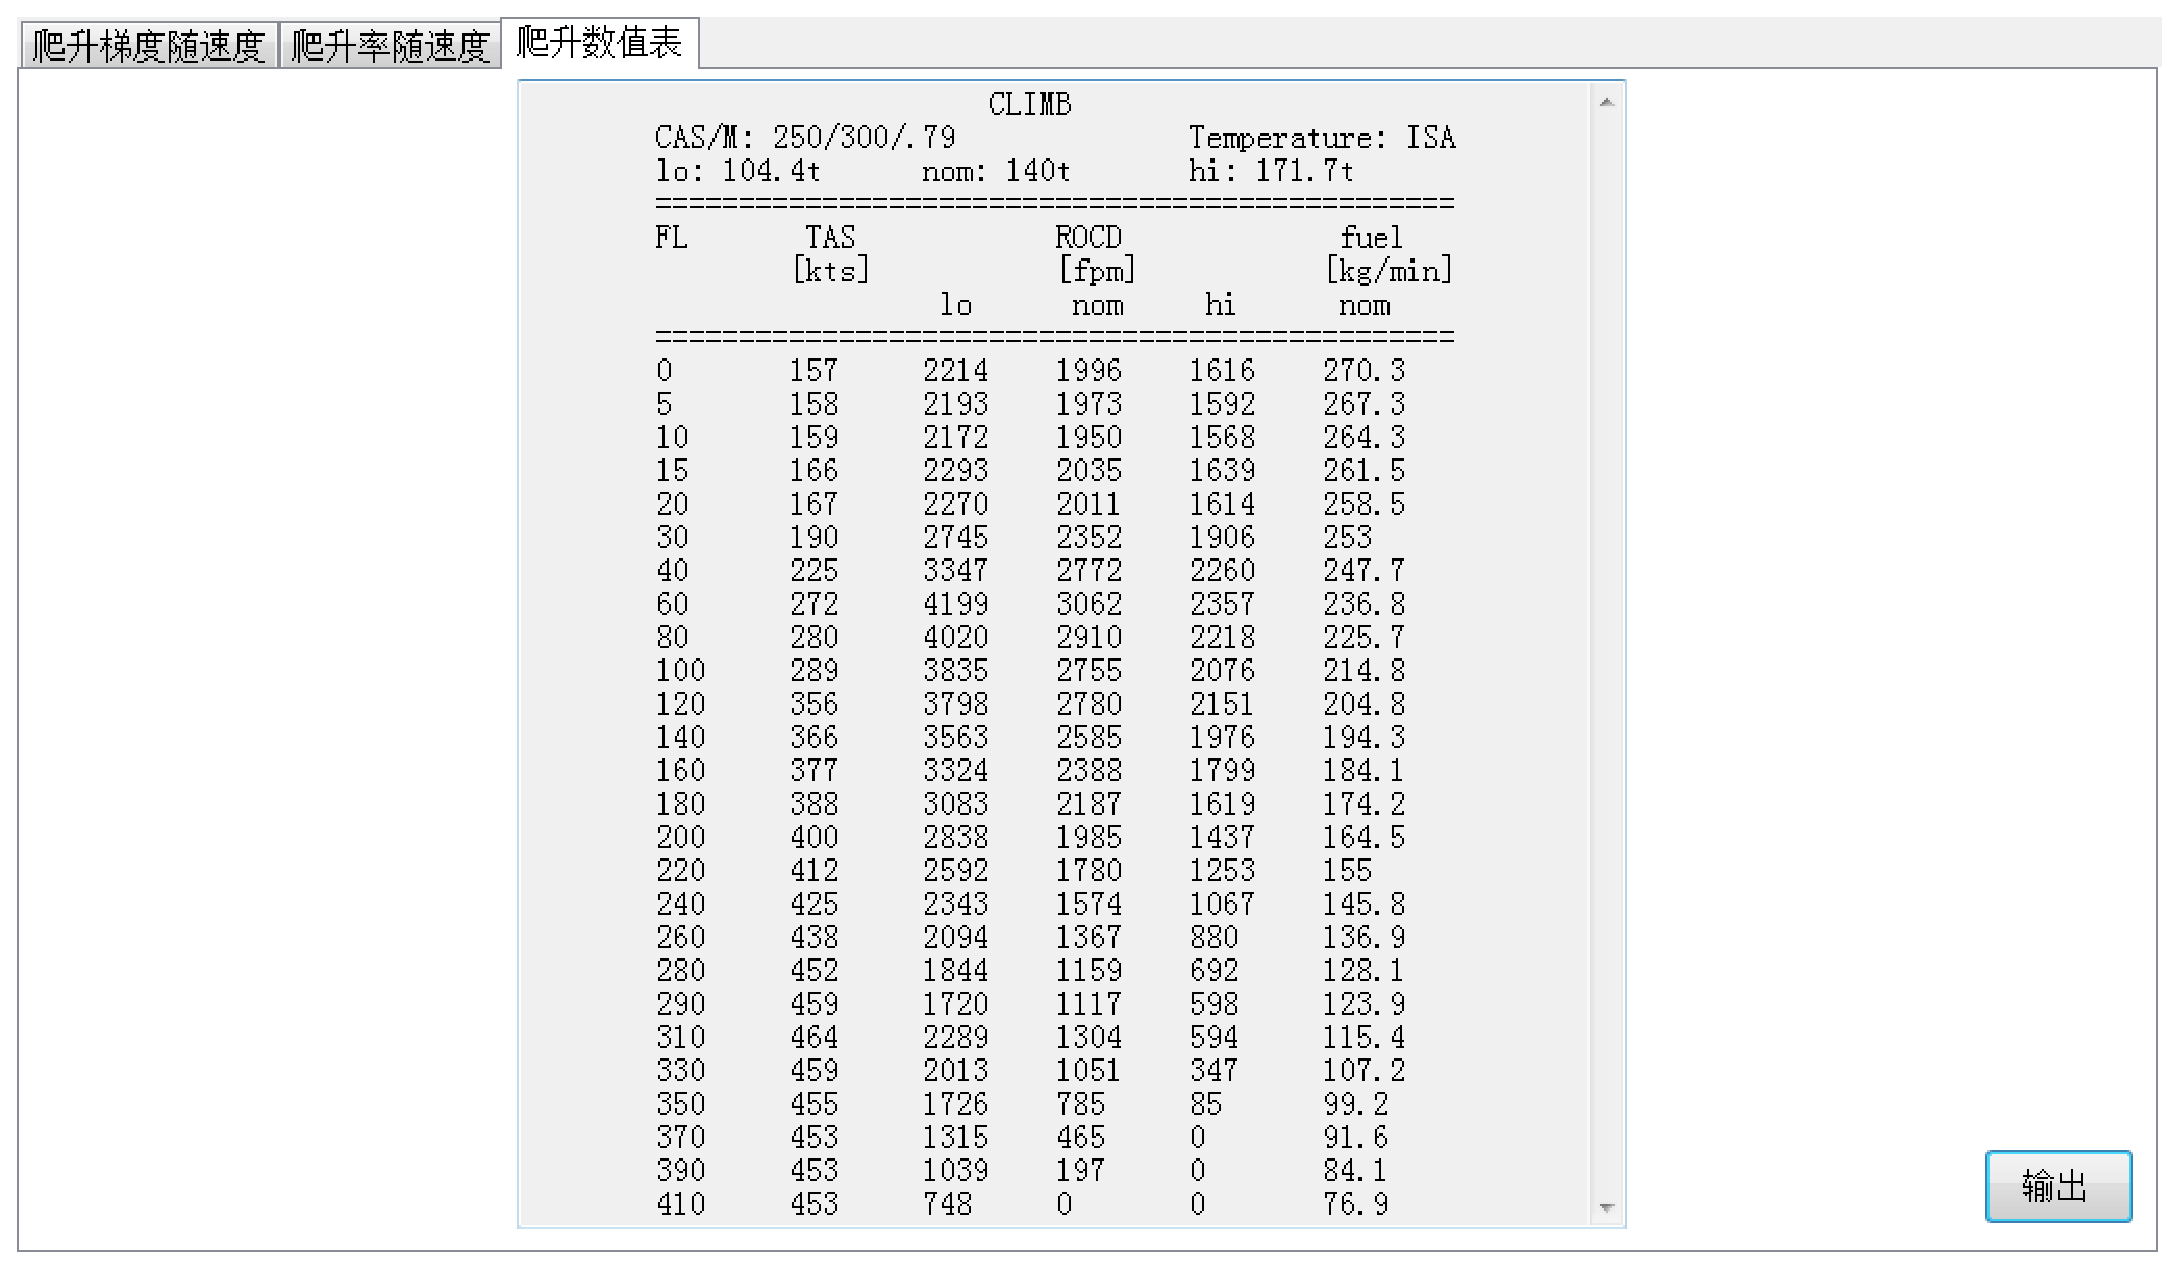
\includegraphics[width=0.8\textwidth]{pic/climbtable.eps}\hspace{30pt}
	\caption{空客300-600爬升数值表}\label{climbtable}
\end{figure}


\subsection{巡航阶段}

(1)燃油里程与马赫数曲线及三种巡航方式

将式\ref{SRequ}稍作变形,有

\begin{equation}
SR=\frac{Ma}{ff}
\end{equation}

其中$a$为所在高度音速。

根据上式绘制空客300-600飞机在不同重量下的$SR$\ -\ $M$曲线。如图\ref{cruisetype}所示,可以看到航空器重量减小会使得曲线向左上方移动,曲线上燃油里程的最大值也随之增大。在图中标识出三种常见的巡航方式,具体介绍如下。

($\romannumeral1$)MRC巡航:MRC的巡航方式为按照该重量下的最大燃油里程对应马赫数飞行。表现在图中为一条连接各曲线顶点的连线;

($\romannumeral2$)LRC巡航:由于以MRC巡航的飞行速度接近有利速度$v_{\rm e}$,容易使航空器进入反常操作区,故以较MRC巡航马赫数大的速度飞行。LRC巡航马赫数为燃油里程为其最大值的99\%时对应的速度。选择每条曲线MRC巡航马赫数右侧的部分,将满足$SR=99\%SR_{\rm max}$的点相连,即可得到LRC巡航方式;

($\romannumeral3$)等马赫数巡航:若在飞行中不使用飞行管理计算机(FMC),则应将LRC巡航方式改为等马赫数巡航以减轻飞行员的操作负担。为安全起见,取重量最大时的LRC巡航马赫数,保持此马赫数巡航。在图中表现为从最大重量对应曲线的LRC马赫数开始,向上垂直延伸的一条直线。

\begin{figure}[h]
	\centering
	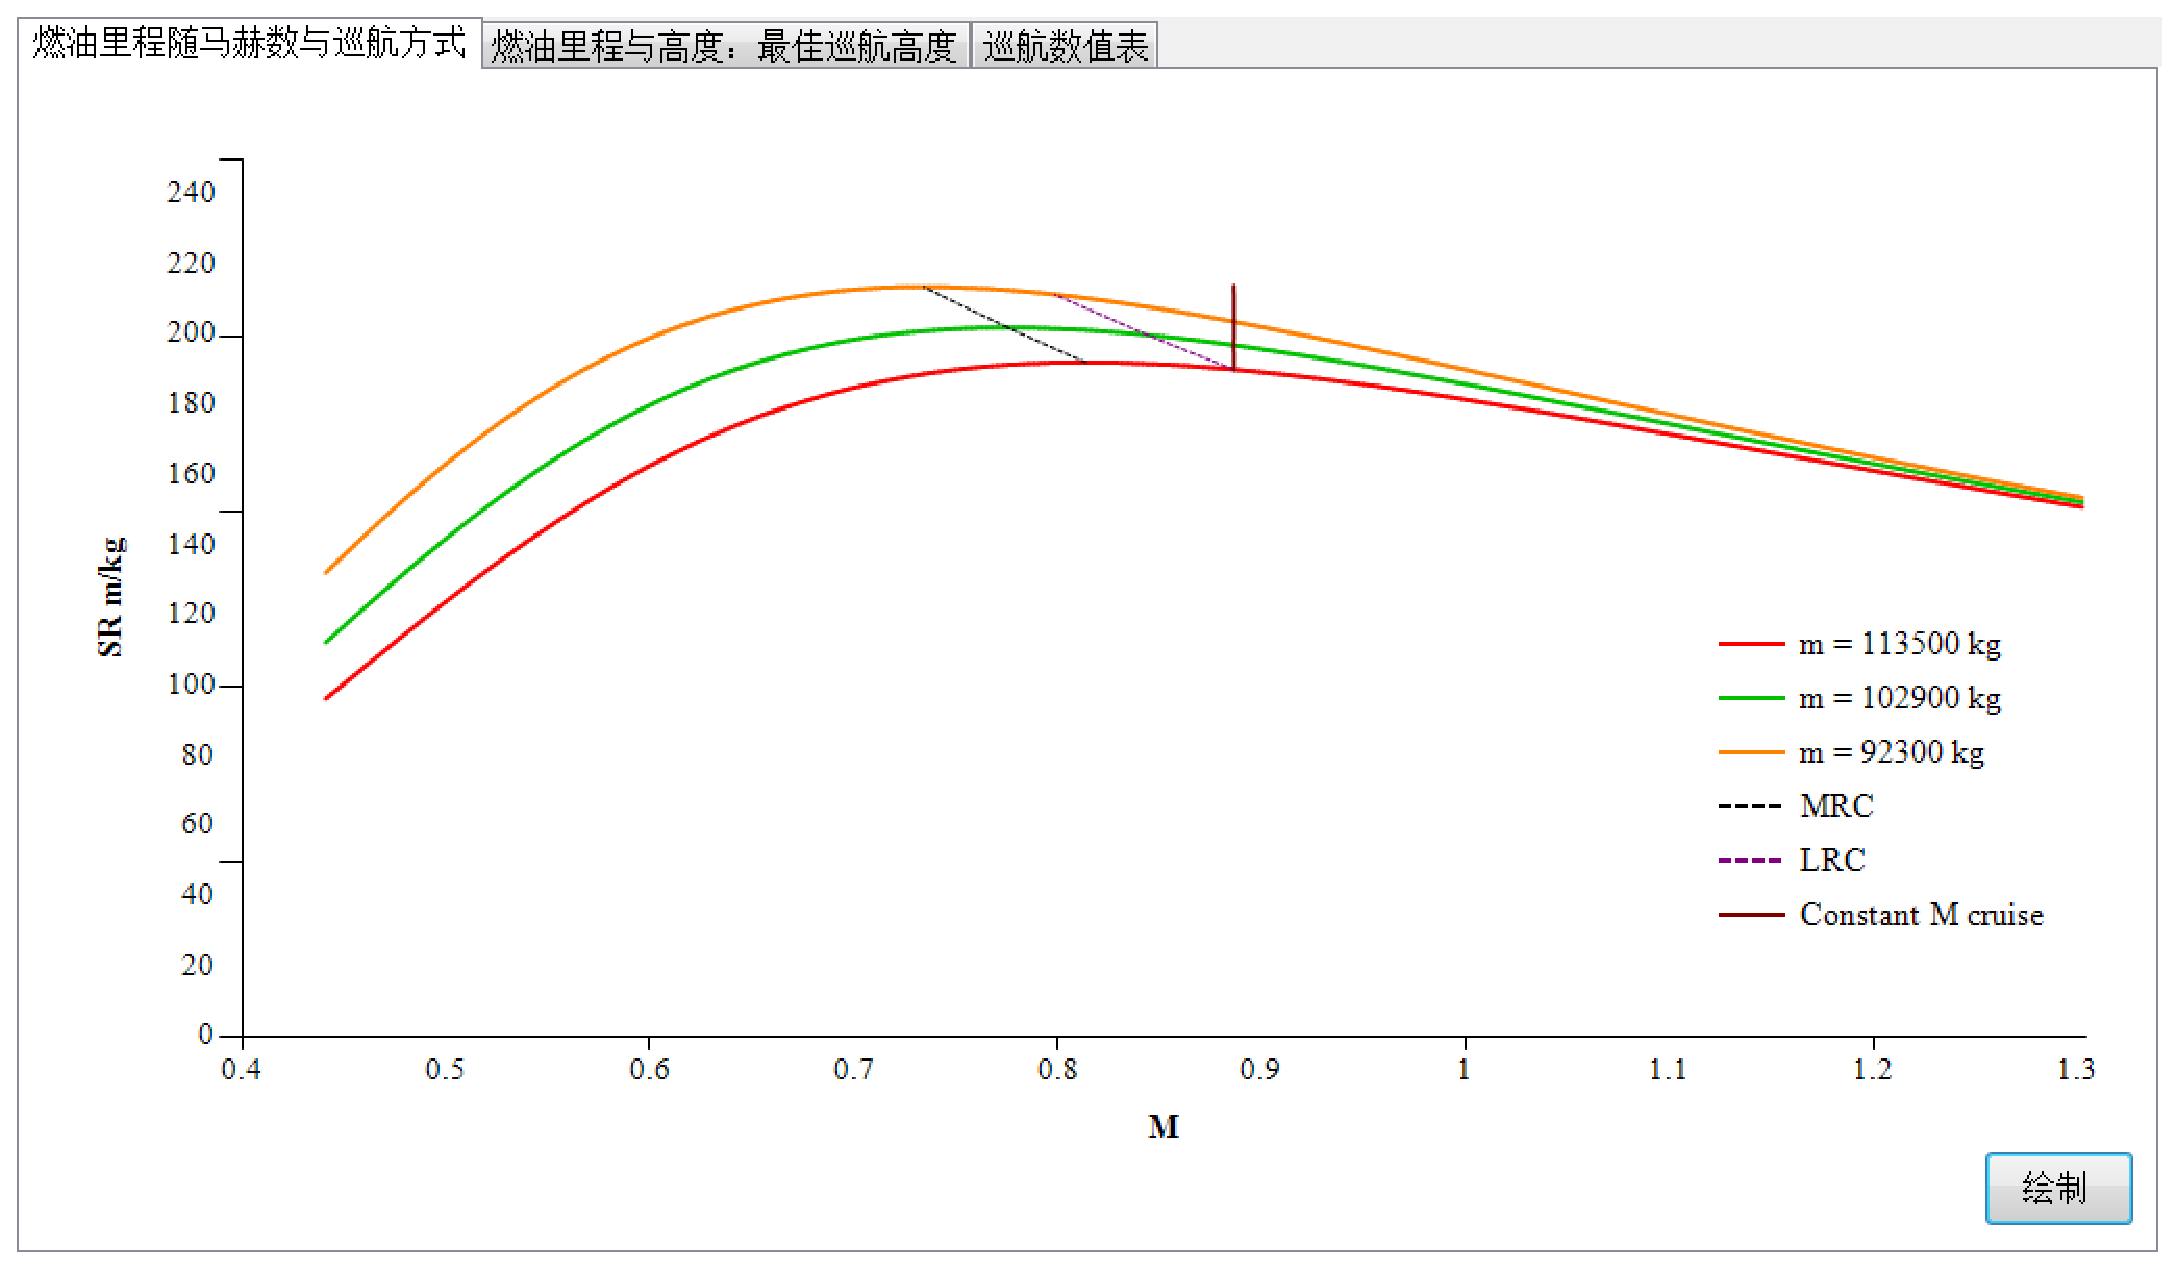
\includegraphics[width=0.8\textwidth]{pic/cruisetype.eps}\hspace{30pt}
	\caption{空客300-600燃油里程与马赫数曲线}\label{cruisetype}
\end{figure}


(2)燃油里程与高度及最佳巡航高度

使用式\ref{SRequ}绘制$SR$\ -\ $h$曲线。为了方便理解,将高度$h$作为竖轴。最佳巡航高度为燃油里程最大的点对应高度,即曲线最右侧点的高度值。

绘制空客300-600的在不同重量下的$SR$\ -\ $h$曲线,如图\ref{optimalaltitude}所示。从图中看出随着航空器重量减小,曲线向右上方移动。连接每条曲线上代表最佳巡航高度的点,可以看到随着重量减小最佳巡航高度将逐渐升高。

\begin{figure}[h]
	\centering
	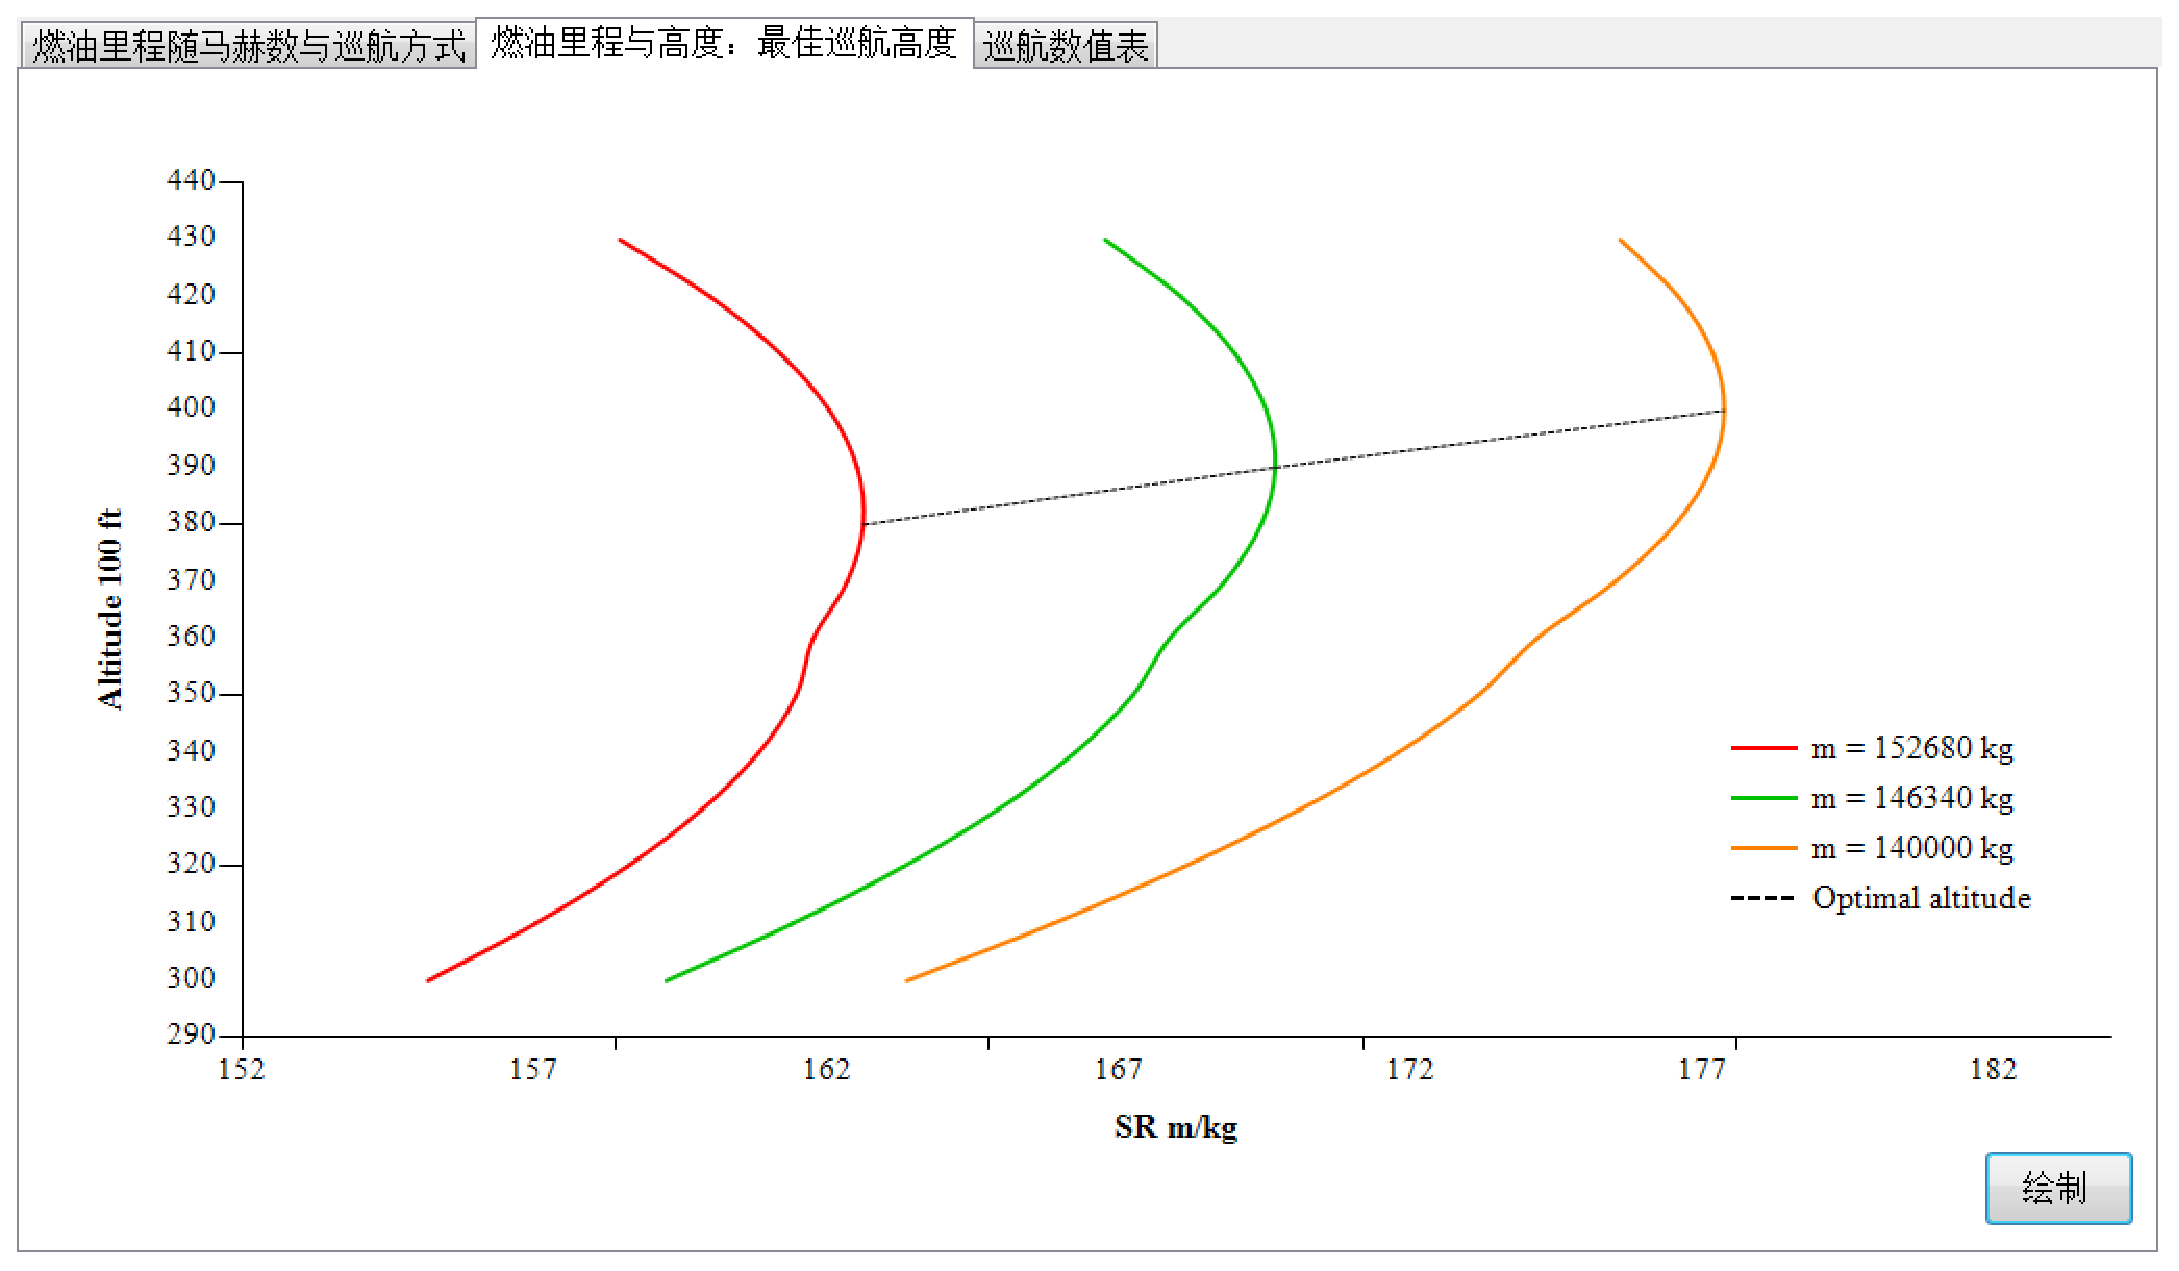
\includegraphics[width=0.8\textwidth]{pic/optimalaltitude.eps}\hspace{30pt}
	\caption{空客300-600燃油里程与高度曲线}\label{optimalaltitude}
\end{figure}


(3)巡航数值表

调用计算函数打印空客300-600飞机的巡航数值表。如图\ref{cruisetable}所示,数值表展示了按等校正空速飞行,各高度的真空速及不同重量下的燃油流量$ff$。值得一提的是,在计算41000\ $\rm ft$标准重量下的燃油流量,以及35000\ $\rm ft$高度以上最大重量下的燃油流量时均使用了最大巡航推力,其他情况均使用正常巡航推力计算。

\begin{figure}[h]
	\centering
	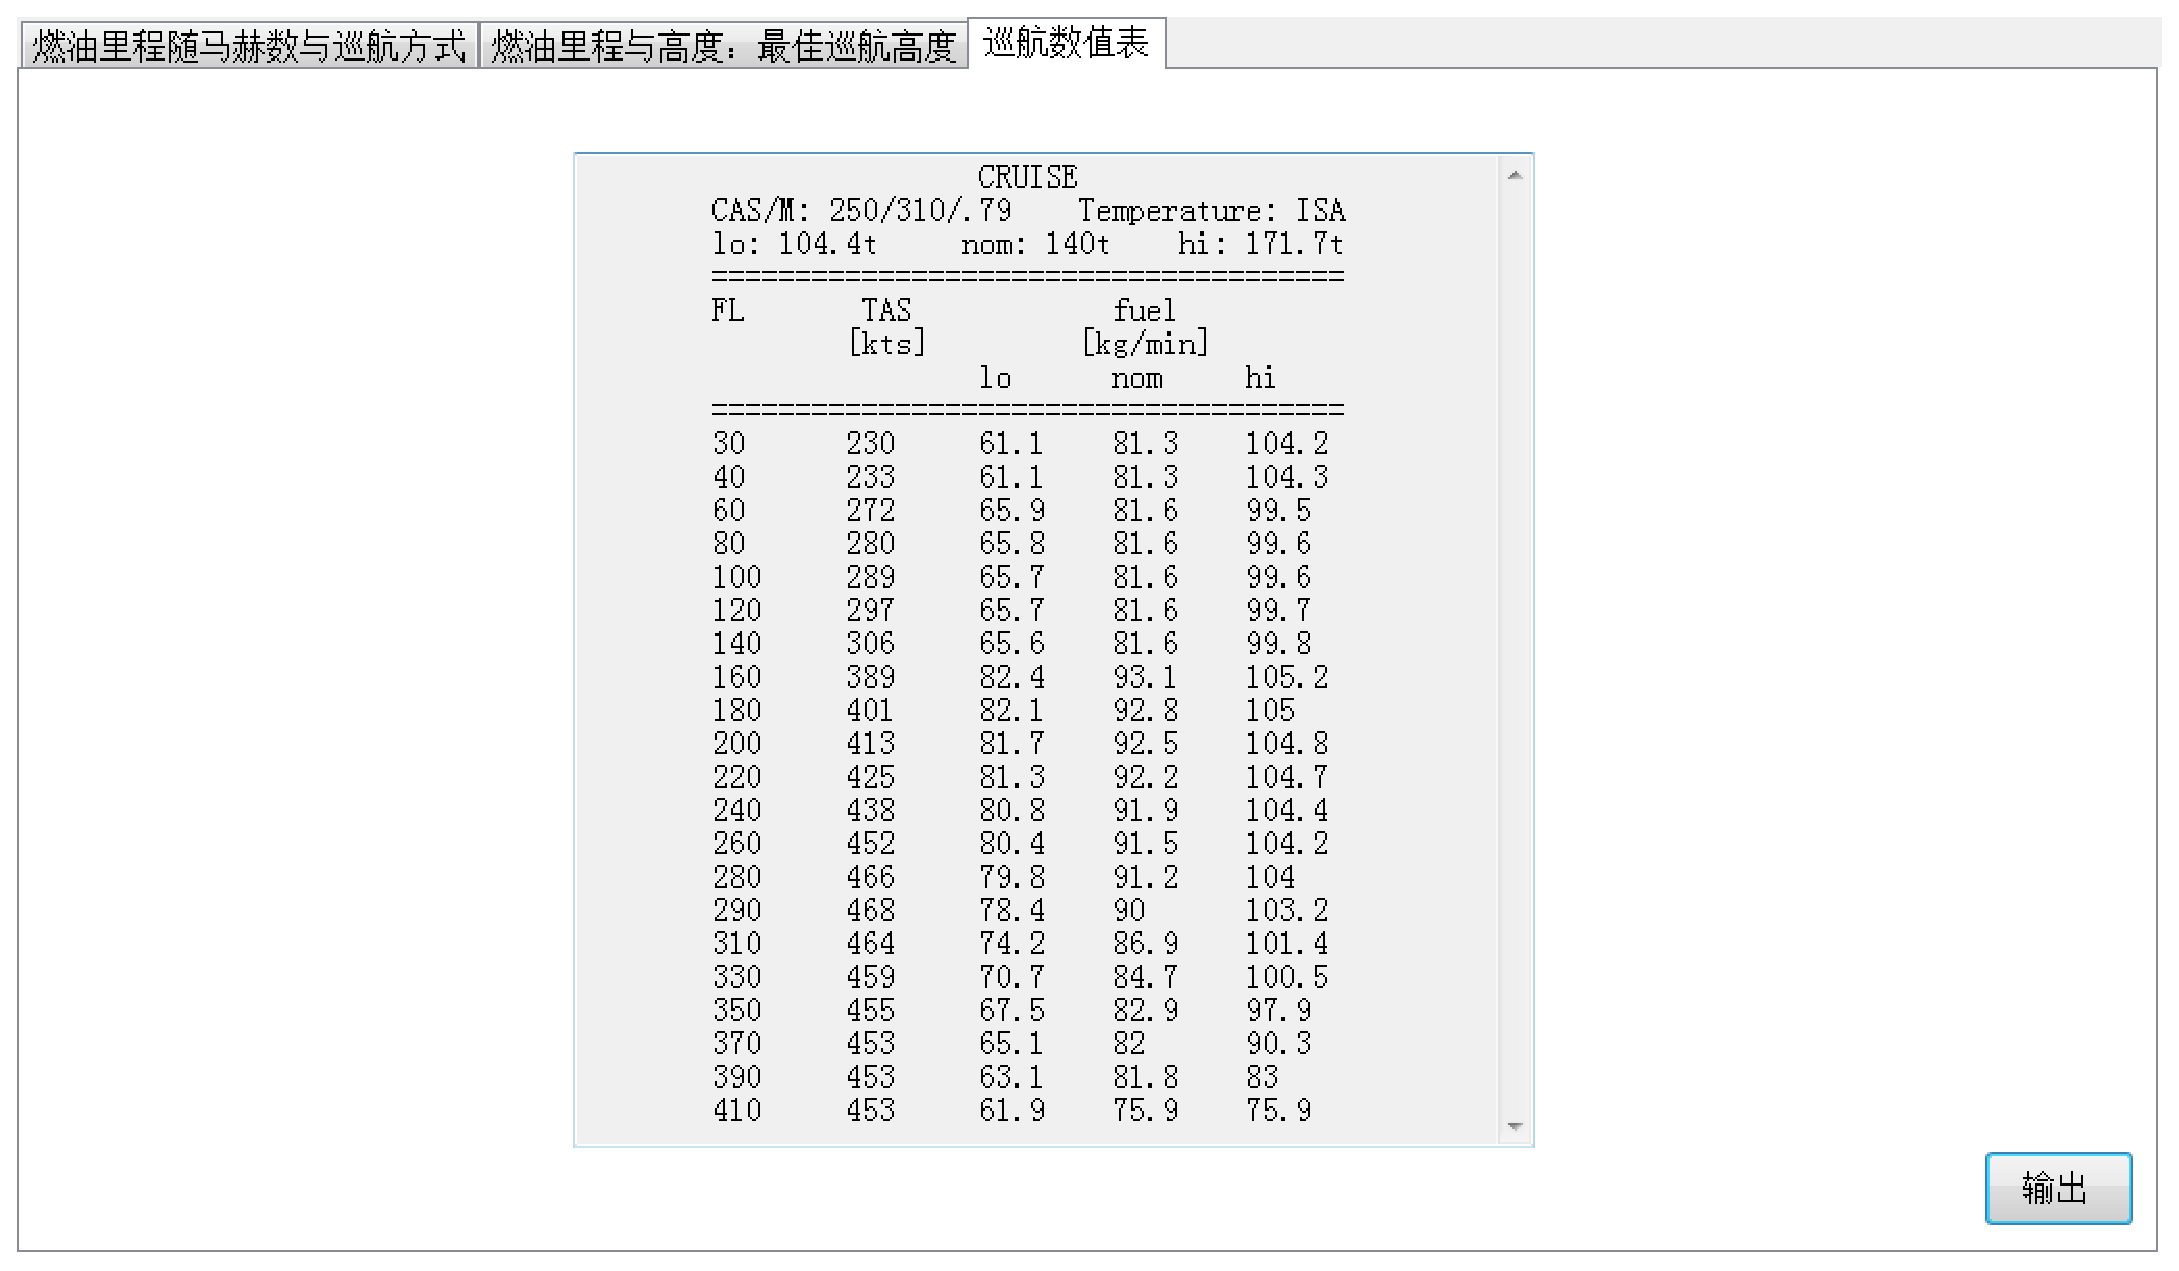
\includegraphics[width=0.8\textwidth]{pic/cruisetable.eps}\hspace{30pt}
	\caption{空客300-600巡航数值表}\label{cruisetable}
\end{figure}


\subsection{下降阶段}

(1)下降梯度随速度变化与飘降速度

为了使下降梯度为正值,将爬升率公式改写为

\begin{equation}
\sin\theta=DG=\frac{D-F_{\rm N}}{W}f\left\{M\right\}
\end{equation}

其中$DG$为下降梯度,$f\left\{M\right\}$为\ref{fM}节中使用的能量转移因子(加速因子)。注意在下降阶段,发动机推力处于IDLE状态,故上式中有

\begin{equation}\label{FIDLE}
F_{\rm N}=F_{\rm IDLE}。
\end{equation}

从上式可以看出下降梯度$DG$与阻力$D$同方向变化。由\ref{Dcurve}节中对阻力随速度变化的分析,可知随速度增大阻力$D$先减小后增大,故下降梯度与速度之间的关系同样也为随速度增加而先减小后增大。

飘降速度为使下降梯度最小的速度。在$DG$\ -\ $v_{\rm TAS}$图中,飘降速度为曲线的最低点。

绘制空客300-600飞机在18000\ $\rm ft$上下降梯度随速度的变化曲线,并在曲线上标注出飘降速度$v_{\rm drift-down}$,如图\ref{dg}所示。

\begin{figure}[h]
	\centering
	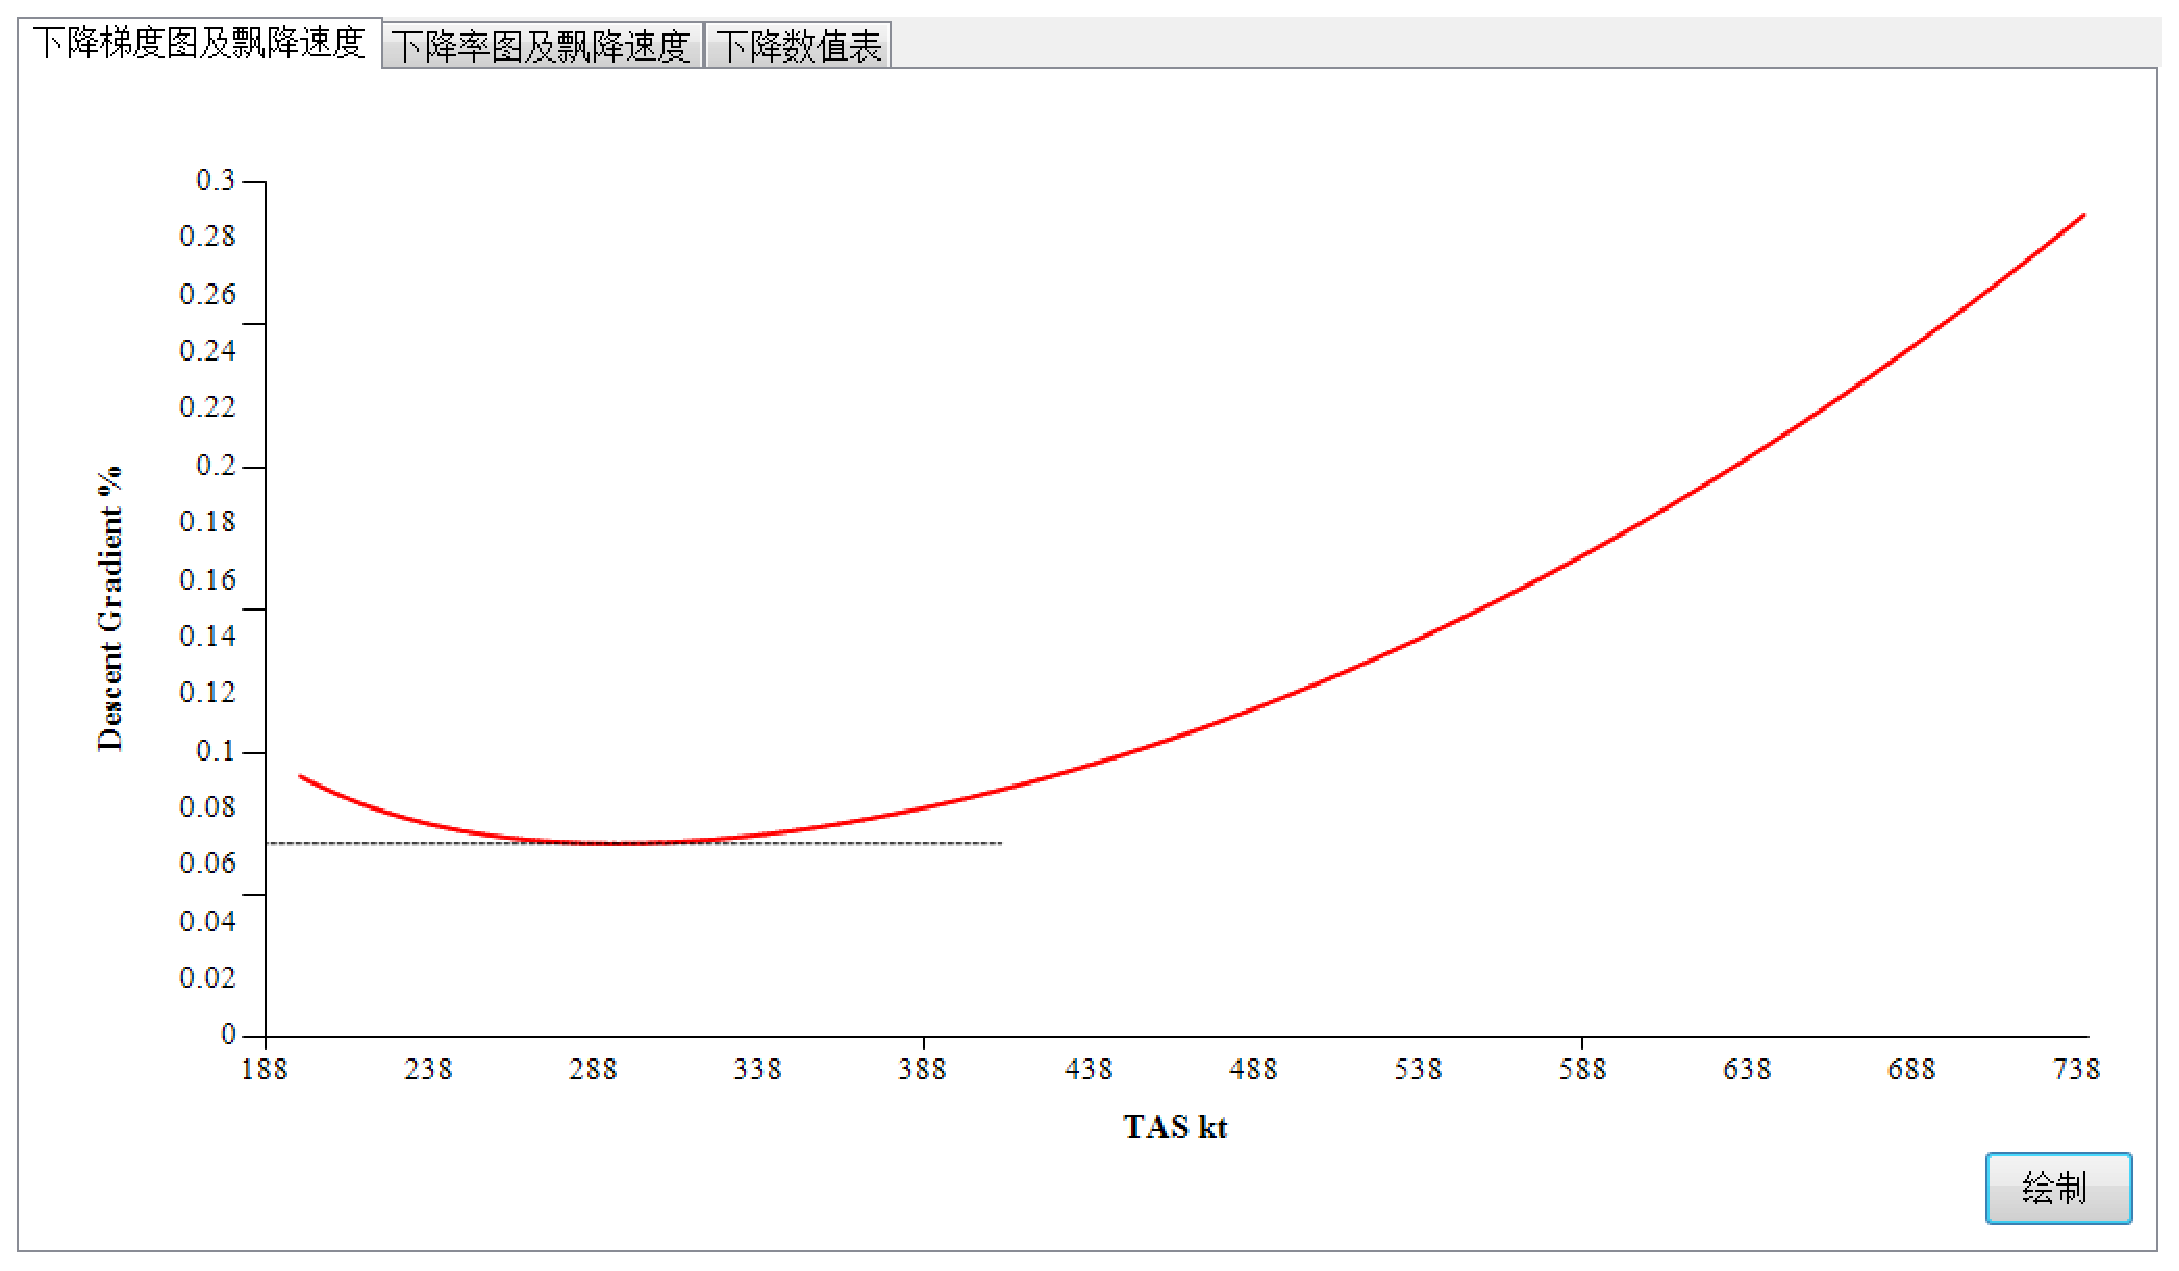
\includegraphics[width=0.8\textwidth]{pic/dg.eps}\hspace{30pt}
	\caption{空客300-600下降梯度随速度曲线与飘降速度}\label{dg}
\end{figure}


(2)下降率随速度变化与飘降速度

由下降率公式

\begin{equation}
ROD=DG\cdot v_{\rm TAS}
\end{equation}

可知随速度增大下降率同样先减小后增大。注意到$ROD$\ -\ $v_{\rm TAS}$曲线的斜率为

\begin{equation}
slope_{\rm ROD}=\frac{ROD}{v_{\rm TAS}}=\frac{DG\cdot v_{\rm TAS}}{v_{\rm TAS}}=DG
\end{equation}

故飘降速度在曲线斜率最小处取得。

绘制空客300-600飞机在18000\ $\rm ft$高度下降率随速度的变化曲线,并标注飘降速度$v_{\rm drift-down}$,如图\ref{rod}所示。

\begin{figure}[h]
	\centering
	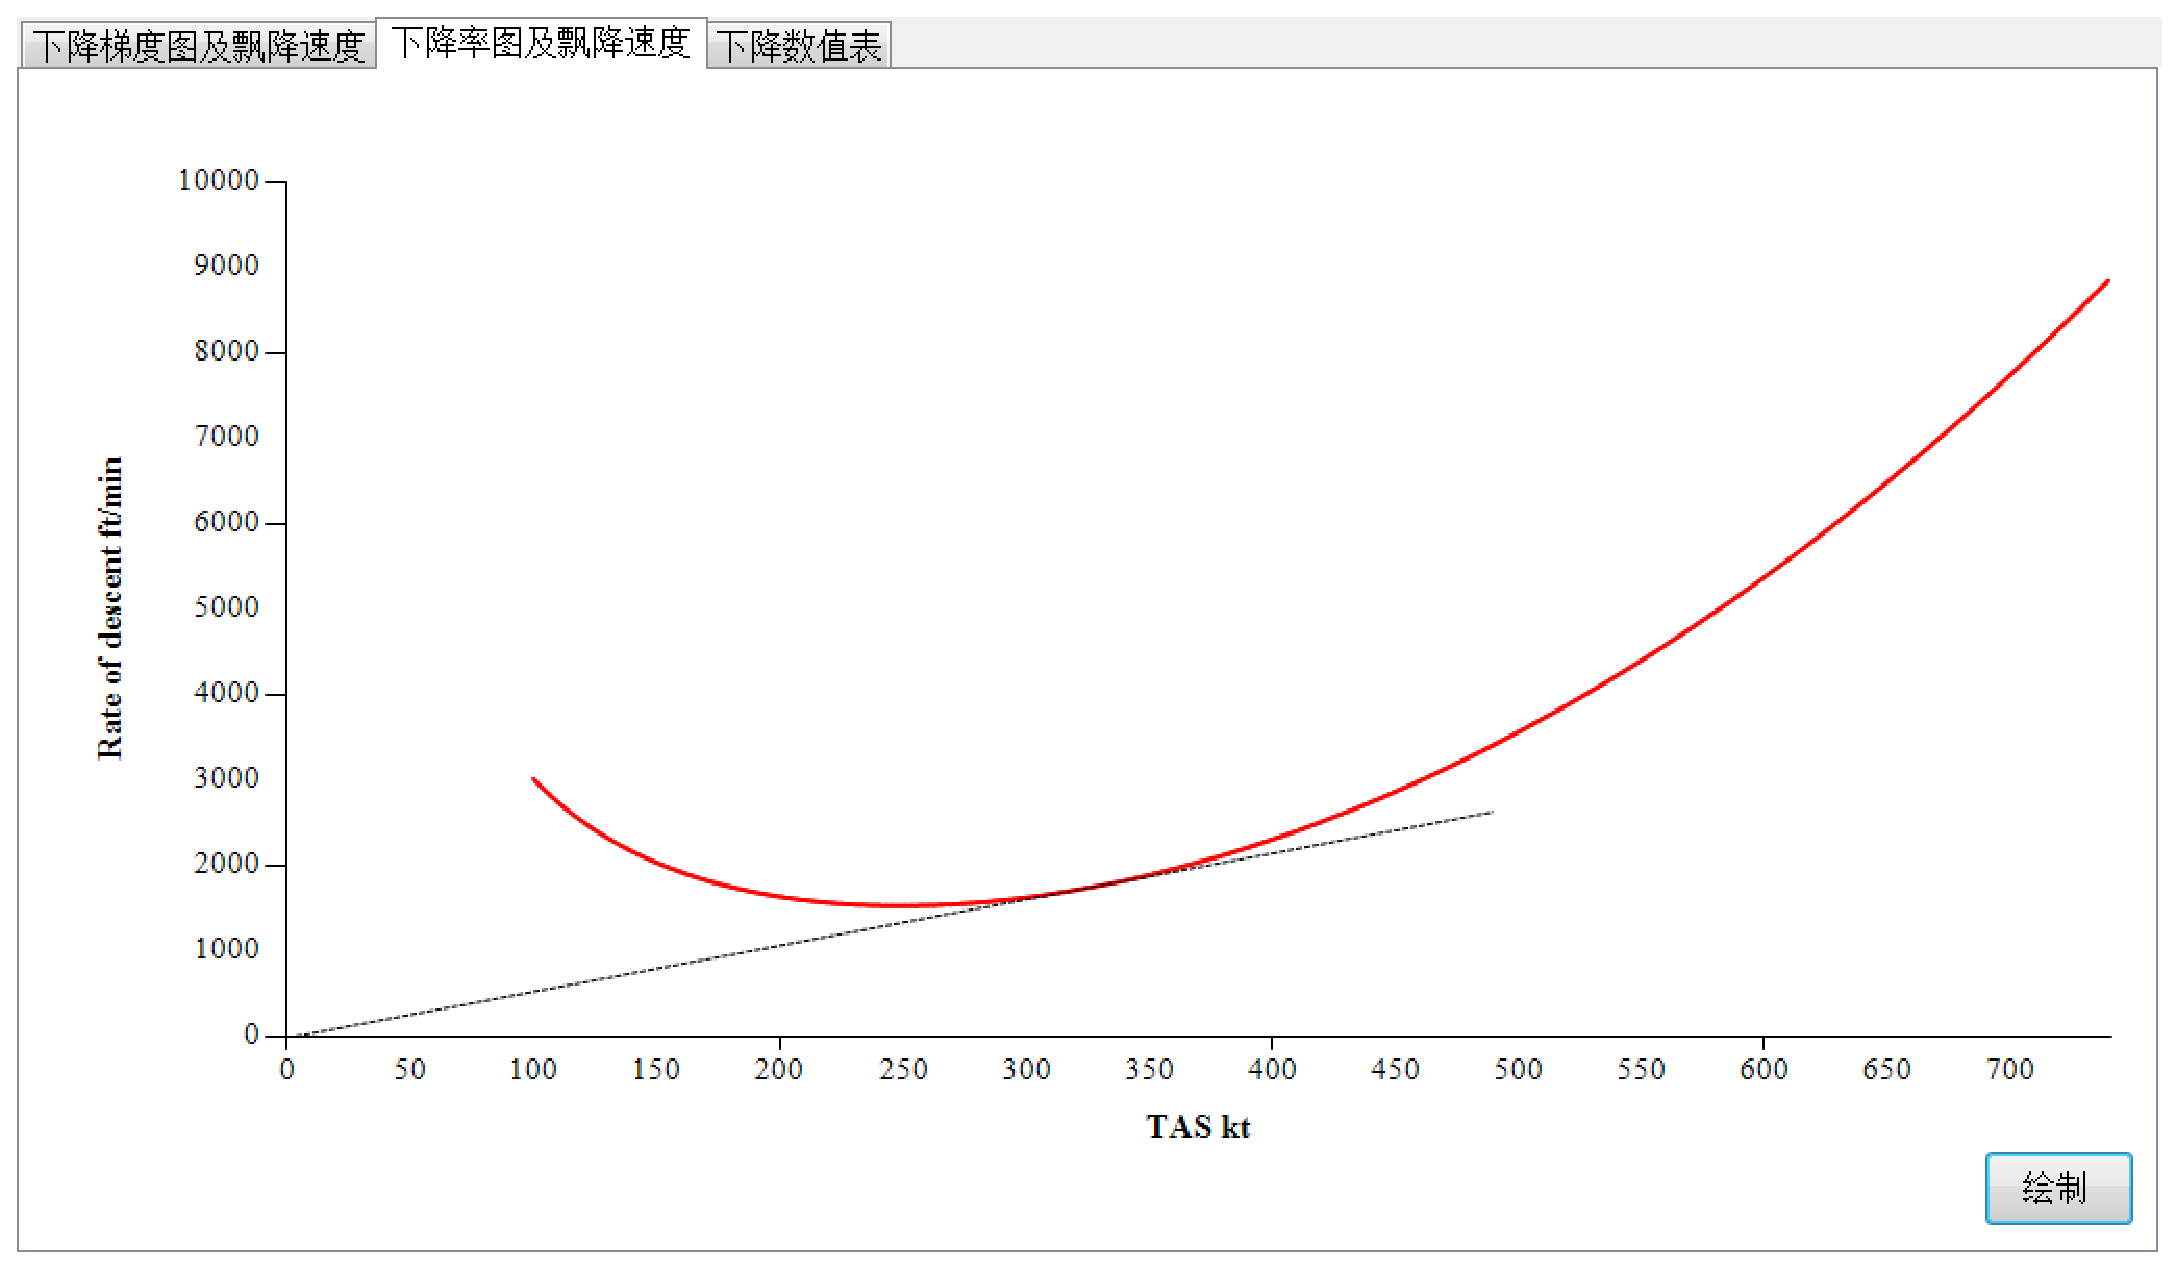
\includegraphics[width=0.8\textwidth]{pic/rod.eps}\hspace{30pt}
	\caption{空客300-600下降率随速度曲线与飘降速度}\label{rod}
\end{figure}


(3)下降数值表

根据调用程序计算函数得到的下降数据制作空客300-600飞机的下降数值表,如图\ref{descenttable}所示。表中展示了按等校正空速飞行,各高度的真空速及航空器处于标准重量时的下降率$ROD$和燃油流量$ff$。值得注意的是,表格中均按式\ref{FIDLE}计算燃油流量。

\begin{figure}[h]
	\centering
	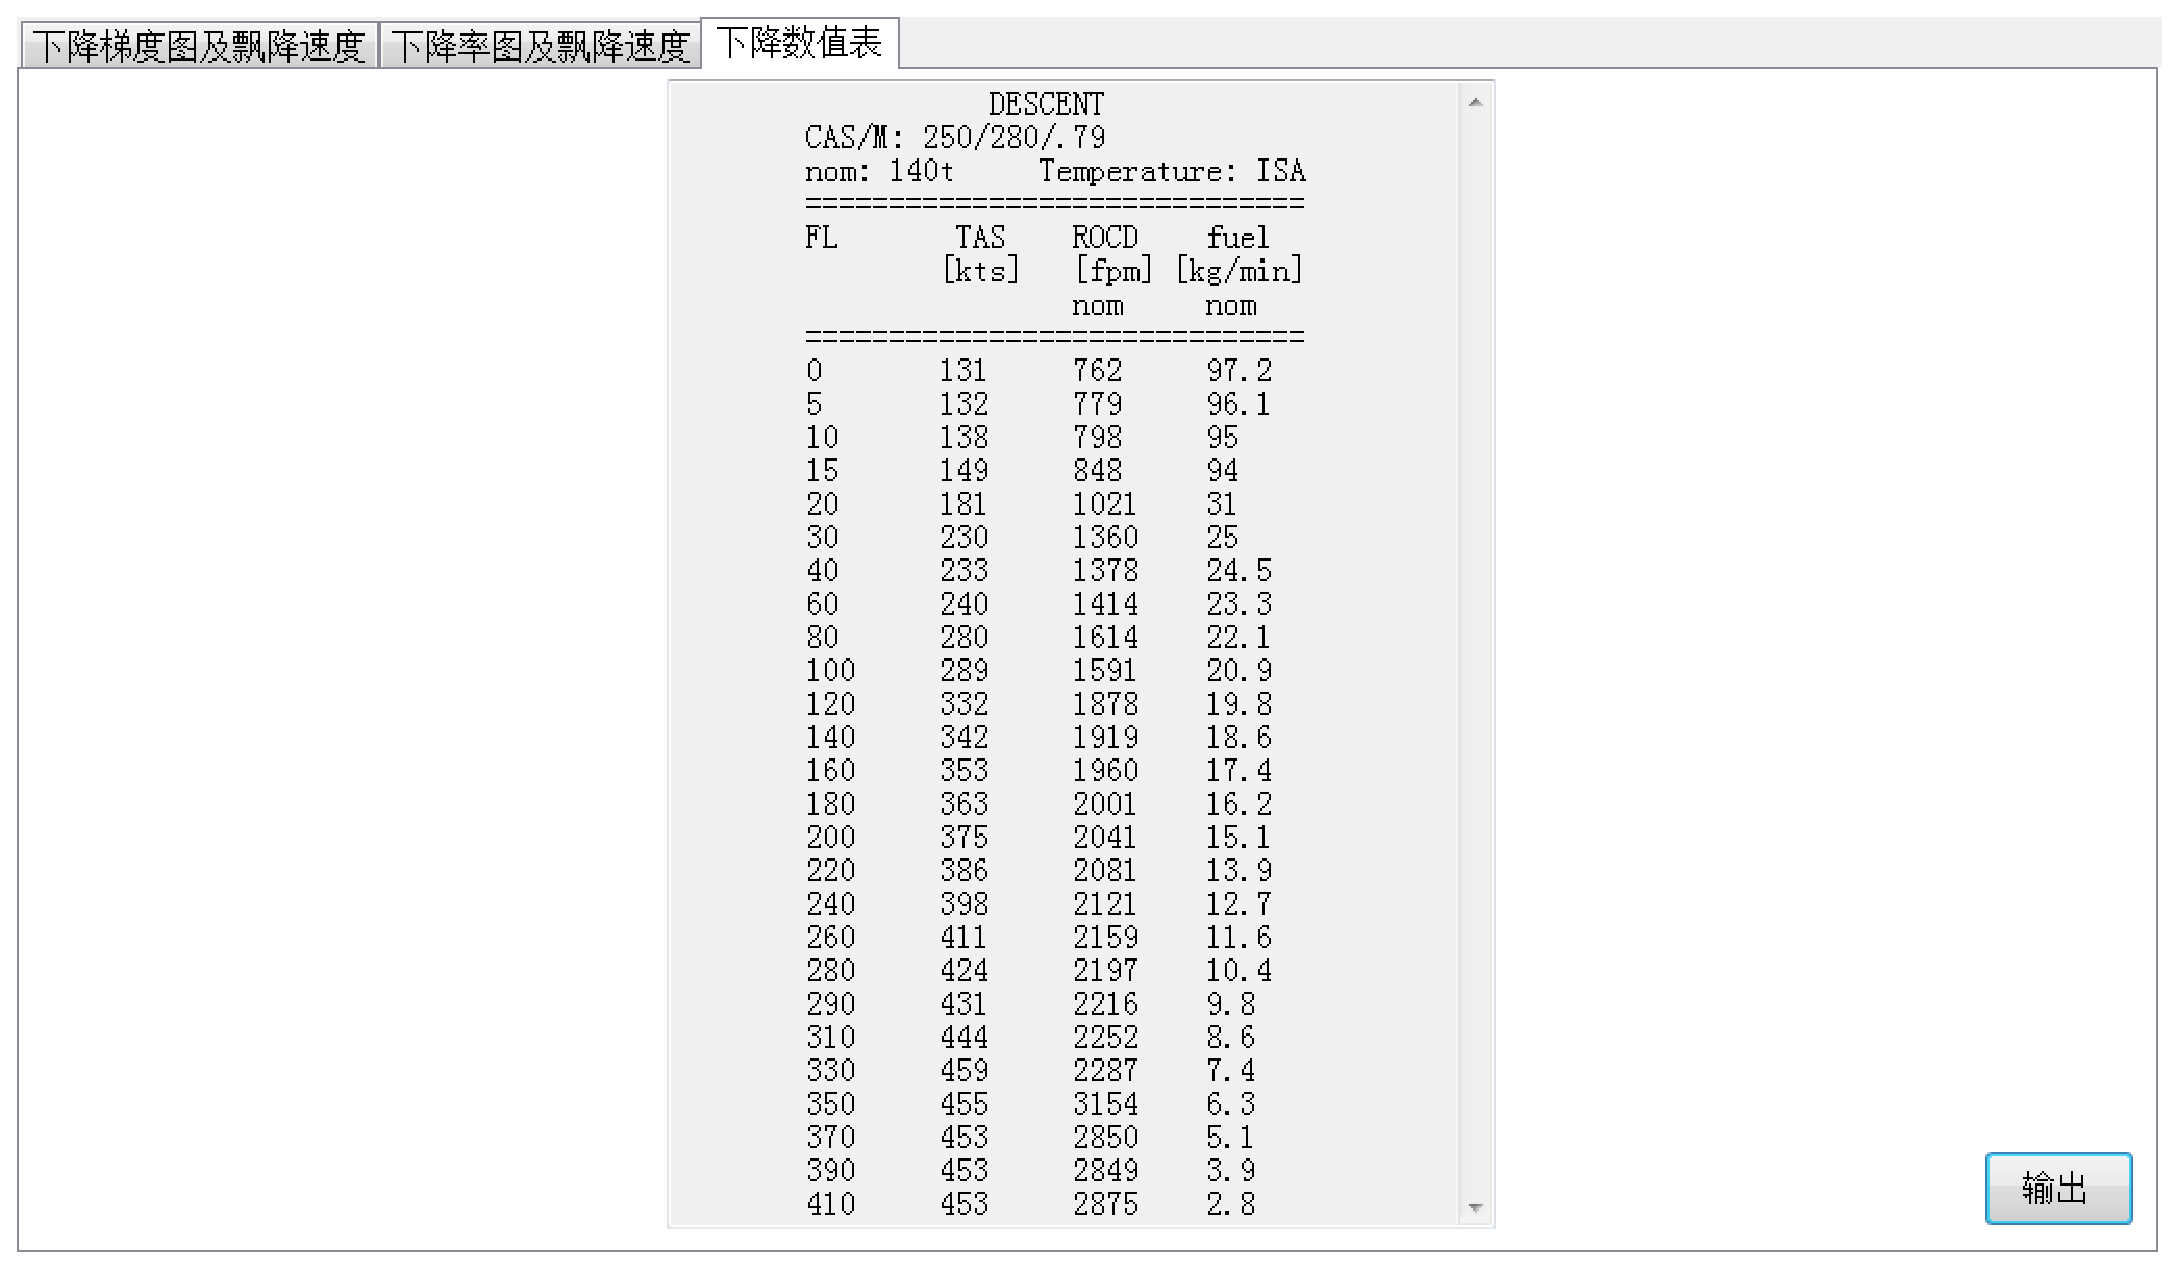
\includegraphics[width=0.8\textwidth]{pic/descenttable.eps}\hspace{30pt}
	\caption{空客300-600下降数值表}\label{descenttable}
\end{figure}


\section{仿真平台软件设计}

在完成基本类及绘制性能图册代码编写的基础上,可以开发性能计算的仿真平台。平台首先读入BADA中的基本机型数据,然后调用基本类进行计算和绘图。

为了保证平台读取基本数据的合法性,编写了一款如图\ref{reader}所示的BADA数据文件读写小工具,将OPF、APF和GPF文件转换为程序可读文本,并在工具中使用正则表达式检查数据合法性。在平台主程序成功读取基本数据后,创建Aircraft基本类,调用类函数可以完成各项性能数据的计算。平台按飞机性能工程课程内容分为气动特性、分析性能方法、飞机运行边界等版块,使用C\# WPF界面的内部控件绘制图线,在画图前可以自行指定图线中的参数,也可直接按默认参数绘制。在指定参数时为保证输出图线正确,平台使用了正则表达式检查输入参数的合法性,并将参数的可取值限定在了一定范围内。如图\ref{flightenvelopetrimmaxW},指定重量为空客300-600最大重量(171.7 $\rm t$),平台绘制出了该重量下的飞行包线。


\begin{figure}[h]
	\centering
	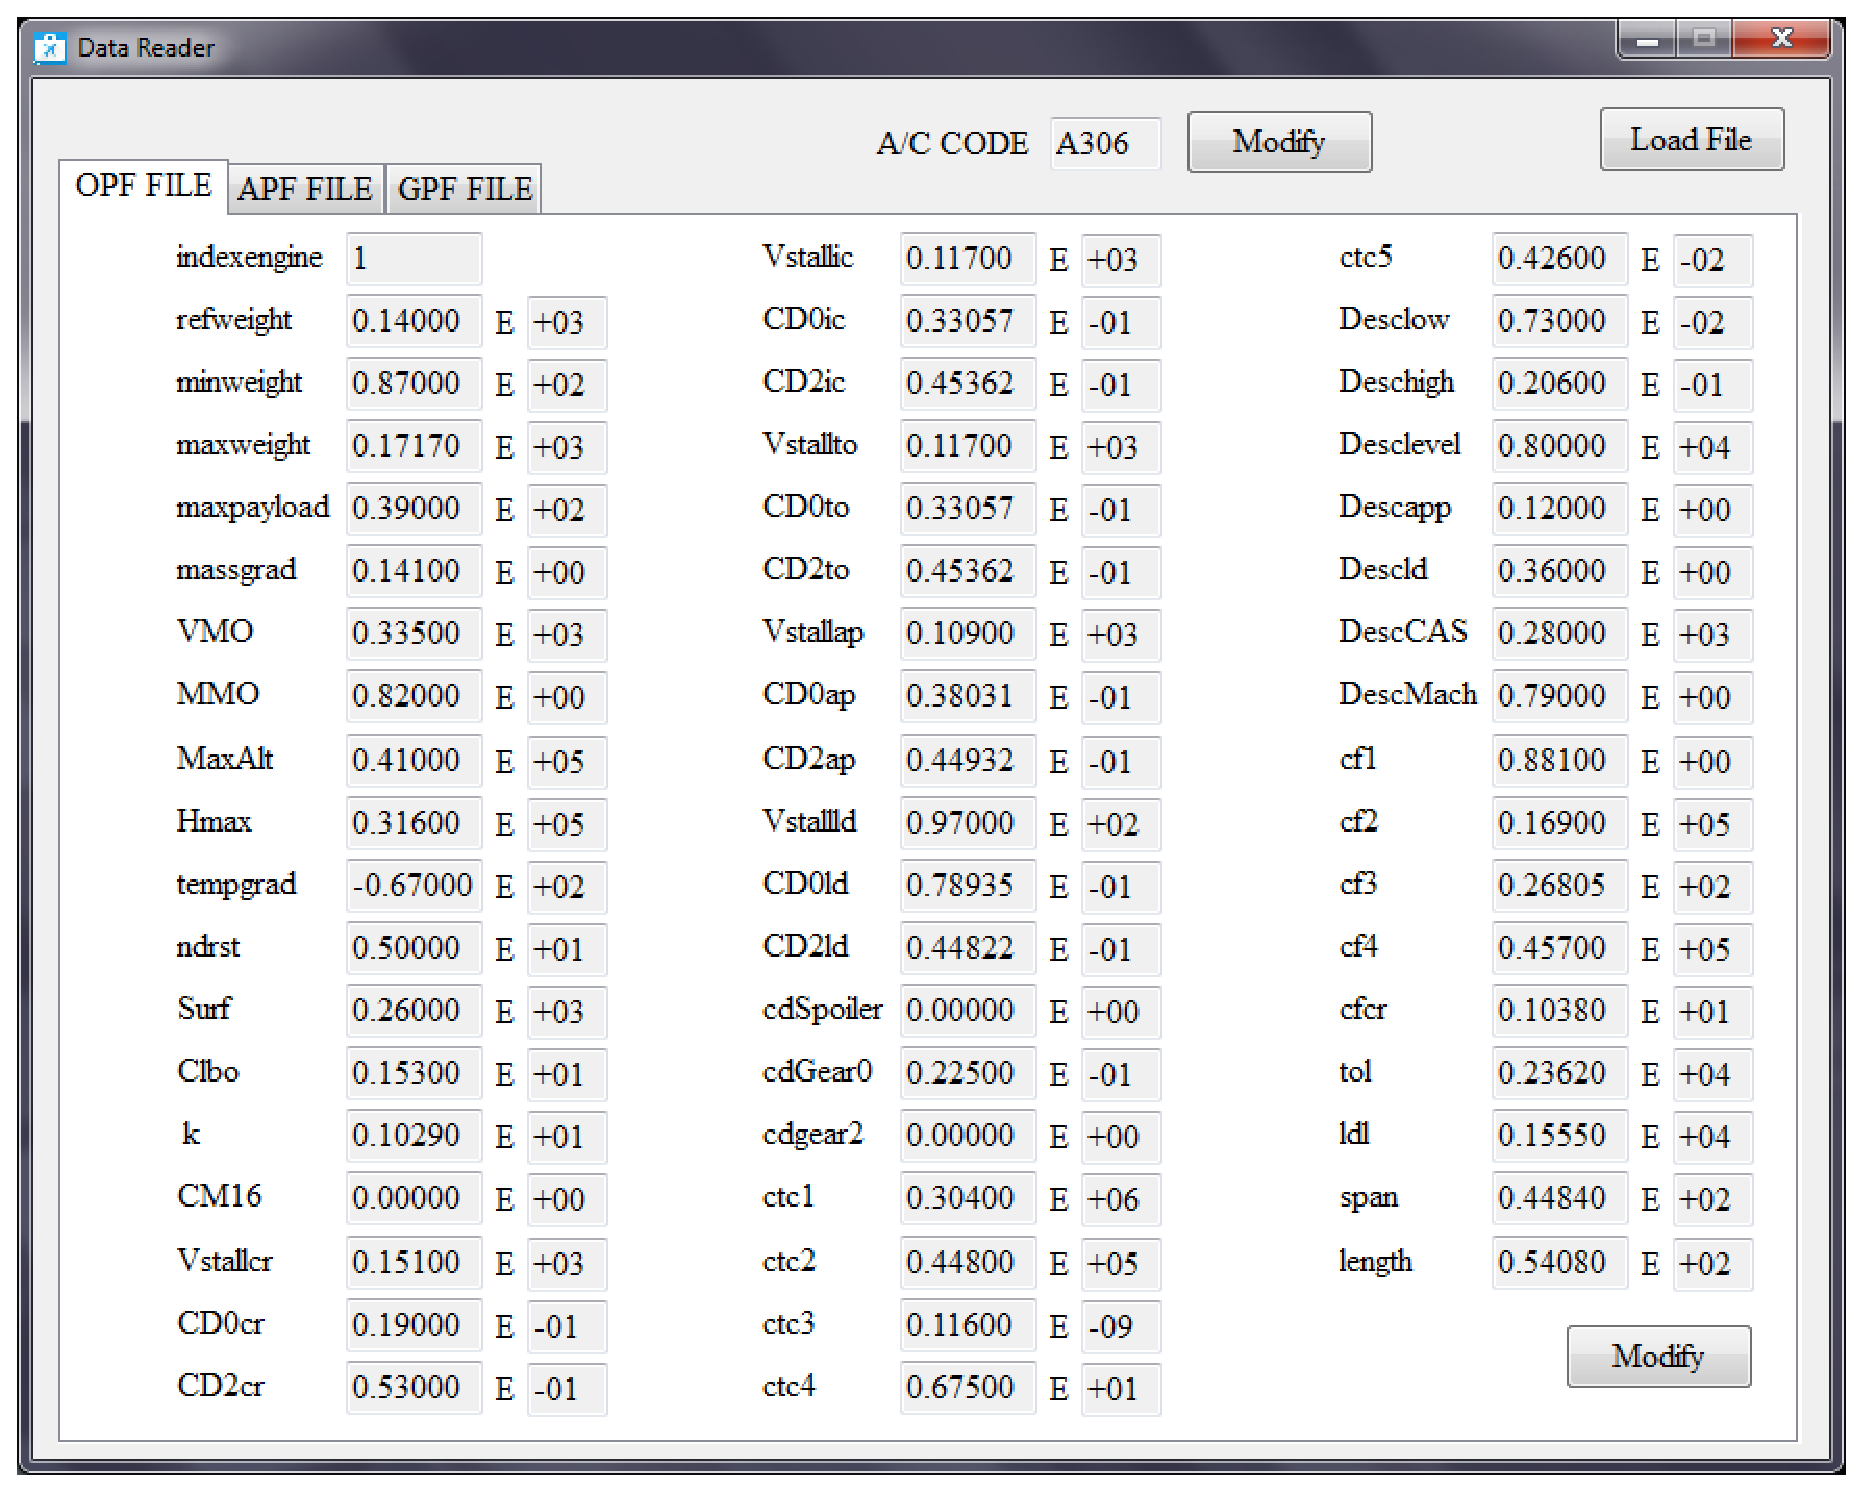
\includegraphics[width=0.9\textwidth]{pic/reader.eps}\hspace{30pt}
	\caption{BADA数据读写小工具}\label{reader}
\end{figure}


\begin{figure}[h]
	\centering
	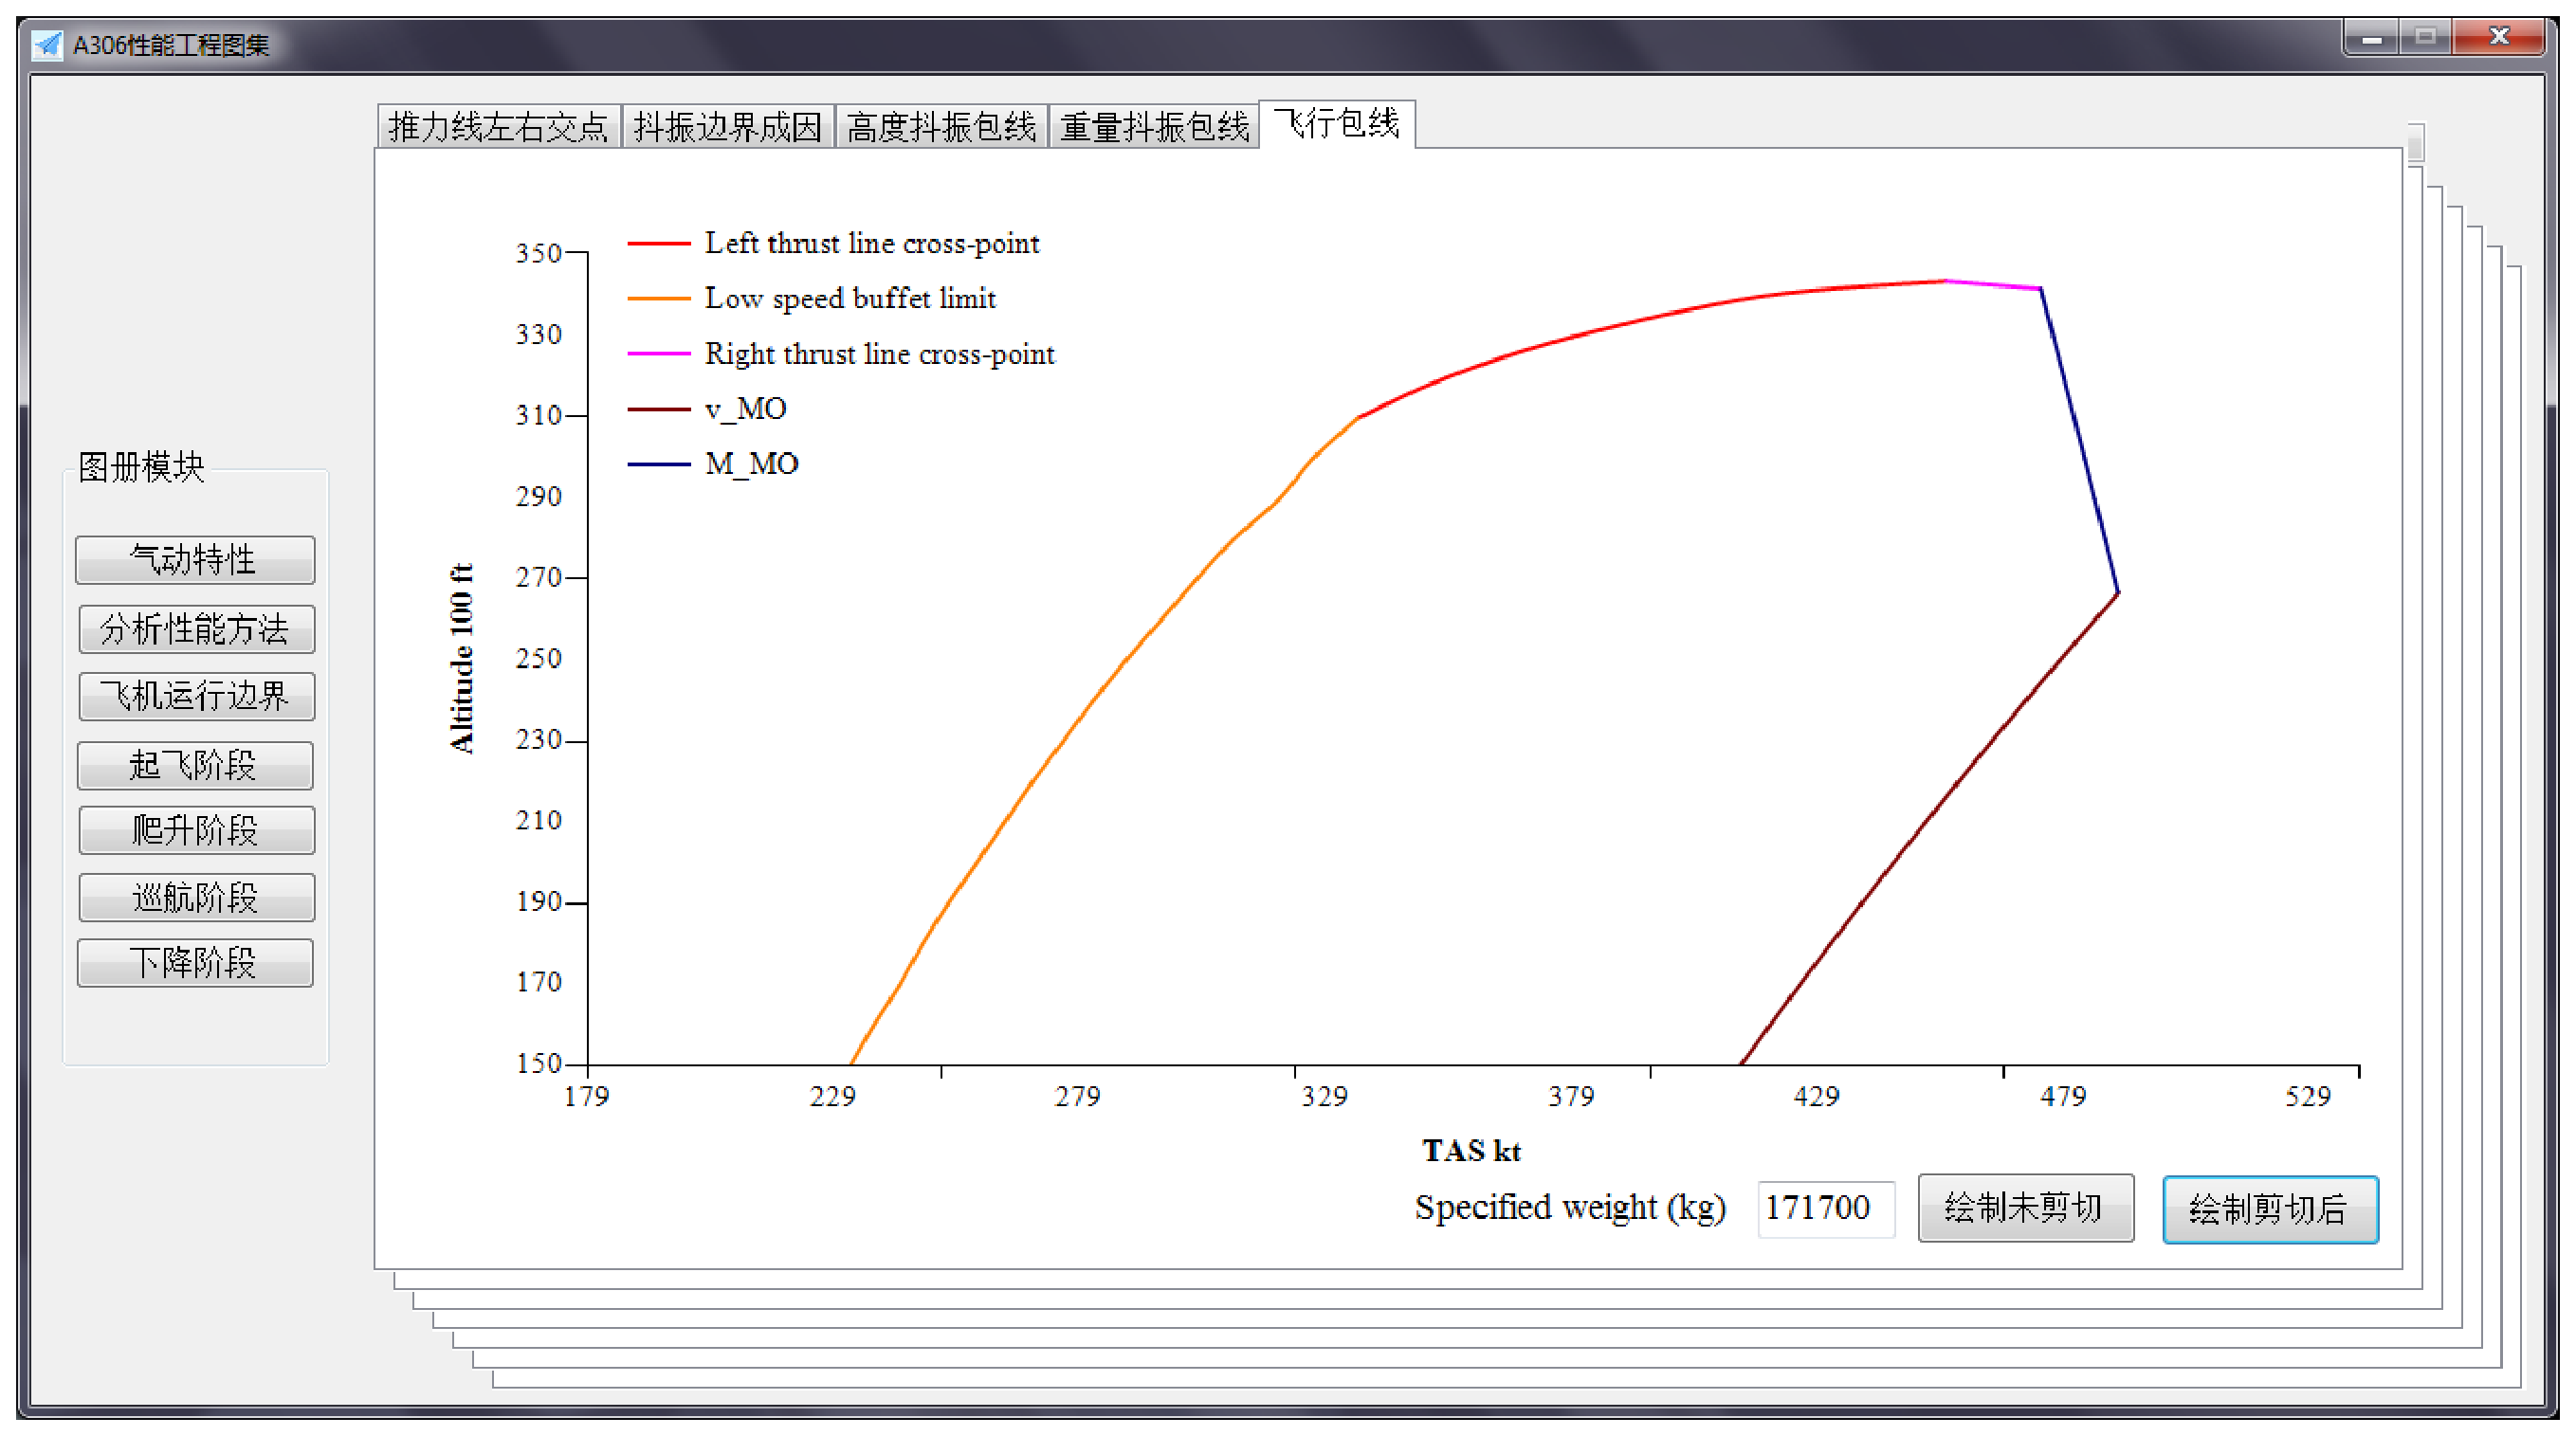
\includegraphics[width=0.9\textwidth]{pic/flightenvelopetrimmaxW.eps}\hspace{30pt}
	\caption{空客300-600在最大重量下的飞行包线(取交集)}\label{flightenvelopetrimmaxW}
\end{figure}


平台软件的开发与代码编写并非核心工作,这是因为制作该平台的目的是为了帮助学习飞机性能的相关知识。本章开发的性能计算仿真平台在结果的精度上不够高,但可以为学习性能工程课程提供基本正确的实证图象。



\chapter{结论}

飞机性能是民用喷气飞机领域中的重要研究课题。飞机在各阶段的性能计算与评估贯穿民航运输工作的始终,同时也是民航院校教学的重点。在学习飞机性能工程课程时,发现在教学中多使用定性的分析方法,在推导性能计算公式后,推测曲线的变化趋势并作出草图。而课程选取民航客机运行手册中的性能图集缺少具体数据,且无法通过调节参数来观察其他情况下的性能曲线。本文整理性能研究模型中的计算公式,编写性能计算基本类,根据性能工程课程内容绘制性能图册,开发了一款飞机性能计算与仿真的平台软件,弥补了实证图象的缺失。具体成果如下:

(1)通过对欧洲空管中心建立的BADA 3.7模型进行梳理,研究飞机的高速飞行性能,对其中涉及的性能计算公式编写成为基本类计算函数。程序读入BADA模型提供的基本机型数据后,即可输入函数所需的参数并调用函数计算各项性能数据。经模型使用手册给出的性能数值表验证,基本类函数的计算结果准确度较好;

(2)研究飞机的低速性能时,由于BADA模型并未提供相应的分析方法,转而采用《Civil Jet Aircraft Design》一书中的低速性能计算模型。在整理起飞距离、平衡场长和着陆距离的计算公式基础上,编写基本类函数。经与BADA 3.7机型基本数据文件比对,计算结果吻合程度较好;

(3)根据性能工程课程中各种性能图线的计算公式,调用基本类函数计算空客300-600飞机的性能数据,并在C\#的WPF界面中利用内部控件绘制图线。最后开发了一款仿真平台,在读入合法的基本参数文件后按照性能工程的课程内容制作性能图册。

性能计算使用了较为粗糙的模型与计算公式。与航空公司提供的性能手册或实际运行的真实数据相比,调用基本类得到的计算结果精确度较差,仿真平台根据这些数据绘制的性能图线也比较粗略。如果采用更加准确的飞机性能计算模型,会使得出的结果更加符合现实情况。另外,理论上仿真平台应可以正确地完成任意导入机型的性能计算和性能图线绘制。然而,这一点在缺乏大量使用反馈和调试工作的情况下很难得到保证。

本文研究结果和开发的仿真平台可能存在诸多不足,请各位审阅老师不吝指正。



\begin{thebibliography}{10}
\markboth{}{}
\addcontentsline{toc}{chapter}{参考文献}%将“参考文献加入目录中”
\bibitem{zhengfengmin}郑峰敏. 飞机起飞性能算法[J]. 空军工程大学学报:自然科学版,2019(3):29-32.
\bibitem{guoan}郭安,周洲,祝小平,等. 基于飞行仿真的飞机起降性能计算方法研究[J]. 西北工业大学学报,2019(3):433-442.
\bibitem{liuxiaochuan}刘小川,张俐娜. 民用飞机最大起飞重量的初步确定方法[J]. 科学技术创新,2019(22):56-57.
\bibitem{wenruiying}温瑞英,魏志强,王红勇,等. 民用飞机巡航性能计算研究[J]. 飞行力学,2015(4):289-292.
\bibitem{huihuihui}惠辉辉,李广文. 基于飞机模型的性能计算与管理[J]. 飞机设计,2019,39(2):24-28.
\bibitem{chushaunglei}褚双磊,董奇,刘子昂,等. 民用飞机的飞机性能辅助计算系统设计与开发[J]. 航空计算技术,2016,46(3):79-83,89.
\bibitem{wangruiping}王锐平. 民用飞机性能综合仿真平台研究[J]. 软件导刊,2014,13(09):97-99.
\bibitem{liuwei}刘薇,马雪,孙俊鹏. 飞机爬升,下降与机动飞行性能计算软件的开发[J]. 长沙航空职业技术学院学报,2019,v.19;No.74(03):67-73.
\bibitem{sunj}Sun J,Hoekstra JM. OpenAP: An Open-Source Aircraft Performance Model for Air Transportation Studies and Simulations[J]. Aerospace,2020,7(8):104.
\bibitem{Wasiuk}Wasiuk,M. H. Lowenberg. An aircraft performance model implementation for the estimation of global and regional commercial aviation fuel burn and emissions[J]. Transportation,2015,35:142-159.
\bibitem{BADA}Eurocontrol Experimental Centre. User Manual for the Base of Aircraft Data (BADA) Revision 3.7[R]. EEC Technical/Scientific Report No. 2009-003.
\bibitem{AircraftDesign}Lloyd R Jenkinson,Paul Simpkin. Civil jet aircraft design[M]. Arnold Press,1999.
\bibitem{PerformaceCourse}陈治怀,谷润平,刘俊杰. 飞机性能工程[M]. 北京:兵器工业出版社,2006.
\bibitem{reflabel1}王淼,刘子昂,褚双磊,等. 基于VB的飞行性能辅助计算软件设计[J]. 成都航空职业技术学院学报,2016,32(01):70-73.
\bibitem{reflabel2}刘春,魏辉. 飞机动力学仿真模型误差分析及调整[J]. 计算机仿真,2013,30(3):101-104,246.


\end{thebibliography}


\thispagestyle{plain}
\chapter*{致\qquad 谢}
\addcontentsline{toc}{chapter}{致\qquad 谢}%将“参考文献加入目录中”
\markboth{}{}
本文的完成离不开庄南剑老师的悉心指导和错误指正,在此对老师表示由衷的感谢。同时刘菲老师和温瑞英老师在我完成毕业设计过程中提供了很多帮助,也在此表达对两位老师的感谢。




\thispagestyle{plain}
\CTEXsetup[format={\Large\bfseries}]{chapter}
\chapter*{附录:外文翻译资料}
\addcontentsline{toc}{chapter}{附录:外文翻译资料}%将“参考文献加入目录中”
\markboth{}{}
\begin{flushleft}
	\setlength\abovedisplayskip{18pt}
	Article Source:Transportation Research Part C 98 (2019) 118–138.
	\setlength{\baselineskip}{20pt}
	\setlength\belowdisplayskip{18pt}
\end{flushleft}

\begin{center}
	\setlength\abovedisplayskip{18pt}
	\setlength{\baselineskip}{20pt}
	\sanhao WRAP: An open-source kinematic aircraft performance model
	\setlength\belowdisplayskip{18pt}
\end{center}

\begin{center}
	\wuhao
	Junzi Sun, Joost Ellerbroek and Jacco M. Hoekstra
	
	\setstretch{1}
	Faculty of Aerospace Engineering, Delft University of Technology, Kluyverweg 1, 2629 HS Delft, the Netherlands
\end{center}


{
	\setstretch{1}
	\noindent\xiaosi\bfseries{3. The data}
}

When dealing with aggregated ADS-B flight data, errors often occur. Trajectory data need to be pre-processed and segmented by flight phase accordingly. At the same time, not all parameters can be directly observed. To infer those hidden parameters, certain models and methods need to be designed. In the following two sections, we discuss the methods used for data processing and performance modeling.\\
3.1. Data source

For this research, the input data are primarily based on ADS-B messages that are broadcast by aircraft through Mode-S transponders. However, even with good installation and placement, a single ground-based receiver only has a maximum reception range of around 250 nm (∼500 km). Considering Mode-S line-of-sight availability, it is not possible to capture large quantities of completed flight data with a single ground station. This is especially challenging when dealing with long-range flights. Thanks to networks of ADS-B ground receivers, such as FlightRadar24 (FlightRadar24 AB, 2017), it is possible to gain access to a much larger collection of flight data obtained from ground stations from contributors around the world.
It is also worth noting that in addition to ADS-B data, using the same receiver setup, aircraft positions and velocities can be also obtained from multiple ground stations using Mode-S multilateration. This technology is employed by some ground receivers within the FlightRadar24 network. It is useful for those aircraft that are not yet equipped with ADS-B compatible transponders. However, the availability is limited to areas where air traffic controllers are present and not usable when aircraft are close to the ground.\\
3.2. Trajectory processing

Data collected from ADS-B are usually scattered. Previous machine learning methods proposed by Sun et al. (2017a) have made it possible to extract flight trajectories easily. However, this method can only segment flights into four different phases: on-ground, climb, cruise, and descent.
The work in this paper requires further processing of those segments. To this end, an altitude threshold is applied to the climb and descent trajectory to extract the initial climb and final approach. We consider the climbing section up to 1500 ft to be the initial climb. The final approach starts from 1000 ft toward the end of the descent. Secondly, to avoid the level-flight segments in climb or descent phases being identified as the cruise, we consider that the cruise segment lasts less than five minutes to be level-flight segments. This threshold is selected empirically based on our analysis of a large number of flights. Lastly, an evaluation process is used to examine the data of all flight segments, ensuring a certain level of completeness and continuity in the given time series data.
To ensure the trajectories selected are matched with correctly identify phases, we employ the validation method proposed in Sun et al. (2017a), which checks the number of altering phases. We then examine the altitude at the start and end of each flight phase, as well as the number of data points presented in each phase.\\
3.3. Atmospheric conditions and speed conversions

The velocity provided in an ADS-B message gives the ground speed of an aircraft. However, the accuracy of the model may be compromised as wind is not considered. For example, the seasonal wind and jet streams cause a great bias when modeling the cruise speed, if only the ground speed is considered. In this paper, wind speeds are computed using an interpolation model from Global Forecast System (GFS) Reanalysis data (Saha et al., 2010).
The GFS Analysis model cycles every six hours, producing atmospheric grids using global data assimilation. The grid data are stored at two resolutions (0.5 and 1 degree). Vertically, isobaric levels from 1000 hPa to 10 hPa are provided, divided into 26 layers. In this paper, the U component (west-east direction) and V component (south-north direction) of wind, as well as the temperature of all grid points, are extracted from the datasets. Then 4-D (latitude, longitude, altitude, and time) grids for wind and temperature are constructed.           
After that, an N-dimensional multi-linear interpolation (Weiser and Zarantonello, 1988) is used to construct a linear 4-D interpolated model. As such, wind and temperature can be produced at any position and time. ADS-B positions of all aircraft are mapped with wind vectors from the model to produce the corresponding airspeeds.

{
	\noindent\bfseries{4. Construction of WRAP parameters}
}

After the flight trajectories are sorted and segmented in proper flight phases, they can be used to construct the desired model parameters. For each aircraft type, at least five thousand trajectories are used to give a good level of confidence in the model. This section discusses the methods for extracting these parameters from the trajectory data.\\
4.1. Takeoff

During the takeoff phase, the parameters of most interest are takeoff distance, mean acceleration and lift-off speed.To overcome the large noise in the velocity measurements during takeoff, a second-degree spline is applied to obtain a smoothed velocity sample set. The distance parameters can be derived from aircraft surface position at the starting and ending positions of the takeoff, using the spherical law of cosines, based on the dot product of the vectors from the center of the earth to the positions.
Compared to takeoff distance and average acceleration, the lift-off speed is more complicated to estimate, due to the low data update rate in an aggregated ADS-B dataset. There is usually a gap of a few seconds between the last on-ground data sample and the first in-air observation.
To estimate the exact moment of lift-off, as shown in Fig. 4, an interpolation model is used. Firstly, the vertical rate VS and time stamp at the first in-air observation are used to estimate the time of lift-off. Combining this result with previously calculated acceleration, the lift-off speed can be obtained.\\
4.2. Initial climb

The initial climb phase is defined as the segment from 35 ft until the aircraft reaches around 1500 ft. There are several major configuration changes (retraction of landing gear and flaps) during this short period of time that can affect the performance of the aircraft. However, because the initial climb segment lasts for only a short time, it suffers from having relatively few data samples, comparable to the takeoff phase. The parameters to be studied are aircraft calibrated airspeed and vertical rate. Both parameters can be computed directly from ADS-B data.\\
4.3. Climb

The climb segment starts when the aircraft reaches clean configuration and lasts until the moment when it reaches cruise altitude. As a common practice, aircraft first accelerate to a target CAS and then fly according to this constant CAS. Mach number increases with the increasing true airspeed, as well as the effect of the decreasing speed of sound. When a certain Mach number is reached, an aircraft will fly according to this constant Mach number until its cruising altitude. During the Mach climb segment, a decreasing CAS will be observed due to the decreasing pressure and temperature.
The challenge is to identify the crossover between the constant CAS and constant Mach climb. Knowing the general profile of CAS and Mach number during the climb, it is possible to design a two-step and two-piecewise estimator for extracting this feature from CAS and Mach number profiles.
The crossover estimator consists of two parts: an increasing (quadratic or linear) segment and a constant segment. The quadratically increasing part is designed so that it resembles the general observation that velocity increases with a decreasing acceleration. The constant segment approximates constant CAS or Mach values.
The entire climbing phase in terms of Mach number can be divided into two parts (increasing and constant). The first estimator applies on the entire climb data and uses a least-squares fitting to extract the best CAS/Mach crossover time and constant Mach climb number.\\
4.4. Cruise

Aircraft generally cruise at selected optimal flight levels that are often the most fuel efficient. Optimal cruise altitude changes as aircraft weight decreases and atmospheric condition alters. The calculation of the optimal cruise altitude requires the knowledge of thrust and drag forces, atmospheric conditions, as well as mass of the aircraft. Since the WRAP model deals with the kinematic parameters of the flight, we have to limit the scope of our model. The model focuses on describing the common and maximum values of altitude, speed, and range based on our data.
The common parameters to be modeled are the cruise altitude and cruise Mach number. These two parameters are computed as the mean values respectively during the flight. The initial cruise altitude, is also an interesting parameter that defines the top of the climb. It is computed as the average altitude during the first minute of the cruise.
Aircraft operational boundary conditions such as their maximum cruise altitude, and maximum cruise Mach number, are first computed as the maximum altitude and Mach number per flight. Then the maximum values of the flights from the same aircraft type are used to model the final boundary conditions in the WRAP model. It is worth noting that the obtained parameters representing operational boundary conditions are the maximum values occurring during the operation. They are often within the performance limitations provided by the aircraft manufacturer.
In addition, the cruise range is extracted as an operational reference parameter. Since aircraft rarely fly a direct route between the origin and destination airport, the flight range cannot be calculated as the great circle distance between origin and destination. Due to the noise inherited from onboard GPS receivers, position reports in ADS-B can contain errors (Mohleji and Wang, 2010). When integrating positions along the trajectory, the accumulated error may grow larger. Hence, a first order spline filter is implemented, and then the trajectory is re-sampled and integrated to produce the cruise range.\\
4.5. Descent

The descent phase of the aircraft is comparable to the climb phase. From the top of descent, the aircraft undergoes a constant Mach and constant CAS descent segment before reaching the approach altitude.
The essential parameters to be modeled are: range from top of descent to destination, Mach number during constant Mach descent, CAS during constant CAS descent, crossover altitudes, and vertical rates.
Similar to climb, the constant Mach/CAS descent performance can be modeled by piecewise estimators. It is possible to use the same process as described in Fig. 5. The Mach profile is described using two linear pieces. The CAS profile consists of a linear and quadratic piece due to the high non-linearity in speed for the final approach segment.
At lower traffic densities, it can occur that aircraft follow a so-called Continuous Descent Approach (CDA), which eliminates levelflight segments to reduce fuel consumption and engine noise. Such an approach affects the result of the aircraft performance in descent. This effect is discussed in Section 7.5 in this paper.\\
4.6. Final approach

Due to different control procedures at each airport, it is not easy to generalize the entire approach segment solely based on flight data. However, the final approach segment from around 1,000 ft until landing can be modeled.
The segment of the final approach represents the end of a descent, where aircraft operate at a nearly constant airspeed and rate of descent. The approach speed and Rate of descent are modeled. In addition, the final approach path angle is calculated.\\
4.7. Landing

The landing model is comparable with the takeoff model. Parameters such as touchdown speed, braking distance, average braking deceleration alnd of the aircraft are modeled similarly to the takeoff phase. Approach speed can be observed from the last in-air velocity. Braking distance can be calculated using Eq. (13), and average deceleration can be calculated similarly to takeoff acceleration.

{
	\noindent\bfseries{5. Results}
}

For this paper, the proposed methods have been applied to 17 common aircraft types. Sufficient data were collected for all aircraft. For each aircraft type, this represents around 5000 sets of data per flight phase. In order to better illustrate the modeling of each individual parameter, detailed results from a single aircraft type (Airbus A320) are described according to the previous model specification.\\
5.1. An Airbus A320 example

For each parameter, all three probability density functions (Normal, Gamma, and Beta) are applied using MLE.\\
5.1.1. Takeoff

Three performance parameters are shown in Fig. 9, where the most common values of these parameters are 1.65 km, 165 kt, and 1.93 m/s2, respectively.\\
5.1.2. Initial climb

Two performance parameters up to the altitude of 1500ft, are shown in the first two plots of Fig. 10, where the most common values are 161 kt and 2477 ft/min.
The evidence for quasi-constant airspeed and vertical rate assumption can be seen from the standard deviations per trajectory, shown in the last two plots. It should also be noted that, in general, the vertical rate has larger variances. This is due to the fact that data sources for vertical rate commonly contain a certain degree of uncertainty (Hempe, 2010).\\
5.1.3. Climb

Within the climb phase, the objective is to model the constant CAS/Mach climb profile, as well as the vertical rates in each of the segments of the profile. All parameters are shown in Fig. 11. Most commonly, before the aircraft accelerates to a constant calibrated airspeed of 293 kt, it has a mean climbing rate of 2016 ft/min. Once reaching the altitude of approximately 12 kft, the aircraft then climbs at 1600 ft/min until reaching a constant Mach number of 0.78 at the crossover altitude of 28.9 kft. After that, the aircraft climbs at 1039 ft/min until reaching the cruise altitude. The flight range of the climb phase is also shown in the last plot, which is typically around 257 km.\\
5.1.4. Cruise

During the cruise phase, cruise Mach number, altitude, and cruise range are shown in Fig. 12 respectively. Maximum cruise Mach number, and maximum cruise altitude, can be obtained as the maximum value of cruise Mach number and altitude.
Unlike other performance parameters, the cruise range is spread very widely, where 99\% of flights globally range from 487 km to 4352 km. This reflects the broad usage of the A320. However, most common flights for this type cruise with a range of less than 1000 km operationally.\\
5.1.5. Descent

Similar to climb, the descent phase can also be modeled as a constant Mach descent segment and a constant CAS descent segment. The parameters are shown in Fig. 13. Most commonly, the aircraft starts its initial descent at a constant Mach number of 0.77 and a vertical rate of −1128 ft/min, until reaching an altitude of 31.6 kft. It then starts a constant CAS descent of 281 kt and vertical rate of −1974 ft/min until reaching the altitude 18.9 kft. Then, the aircraft descends with a vertical rate of −1196 ft/min until final approach. The last plot shows the range from top-of-descent to destination, typically around 234 km.
It is worth taking into consideration that the results obtained from the dataset contain both CDA and non-CDA descent approaches.

\clearpage
\thispagestyle{plain}
\CTEXsetup[format+={\centering}]{chapter}
\chapter*{外文翻译资料译文部分}

\begin{flushleft}
	\setlength\abovedisplayskip{18pt}
	文章出处:交通运输研究,2019,C部分98:118-138.
	\setlength{\baselineskip}{20pt}
	\setlength\belowdisplayskip{18pt}
\end{flushleft}

\begin{center}
	\setlength\abovedisplayskip{18pt}
	\setlength{\baselineskip}{20pt}
	\sihao\bfseries\songti WRAP:一个开源的飞机性能动力学模型
	\setlength\belowdisplayskip{18pt}
\end{center}
\vspace{0.05em}
\begin{center}
	\wuhao
	孙俊姿,朱斯特 艾勒布鲁克,雅科 霍克斯特拉
	\setstretch{1.5}
	
	荷兰代尔夫特工业大学航空航天工程学院,2629 代尔夫特
\end{center}

{
	\setstretch{1}
	\noindent\xiaosi\bfseries\songti{3. 数据}
}

处理所有的ADS-B飞行数据时,经常会发生错误。航迹数据需要根据飞行阶段进行相应的预处理和分段化。同时,并非所有参数都可以直接观察。为了推断那些隐藏的参数,需要设计某些模型和方法。在以下两小节中,我们将讨论用于数据处理和有关性能建模的方法。\\
3.1. 数据源

对于本研究,输入数据主要基于飞机通过S模式应答器广播的ADS-B消息。但是,即使安装和放置的很好,单个地面接收器的最大接收范围也只有大概250海里(约等于500公里)。考虑到S模式的视距内可用性,使用一个地面站捕获大量的飞行数据不可能的。在处理远航程航班时,这尤其具有挑战性。由于有ADS-B地面接收器组成的网络,例如FlightRadar24(FlightRadar24 AB,2017年),从世界各地的贡献者的地面站获取更大范围的飞行数据成为了可能。
还值得注意的是,除了ADS-B数据外,使用相同的接收器设置,飞机的位置和速度也可以从多个地面站使用S模式多点测量获得。该技术被一些FlightRadar24网络内部的地面接收器采用。对于尚未配备与ADS-B兼容的应答器的飞机而言,它很有用。然而可用性仅限于有空中交通管制员的区域,并且当飞机靠近地面时是不能使用的。\\
3.2. 航迹处理

从ADS-B收集的数据通常是零散的。先前Sun等一些人(2017a)提出的机器学习方法做到了可以轻松提取飞行航迹。但是,此方法只能将航段分为四个不同的阶段:地面,爬升,巡航和下降阶段。
本文的工作需要对这些阶段进一步处理。为此,将在爬升和下降段使用一个高度阈值来提取初始爬升和最后进近的数据。我们认为1500英尺以下的爬升段是初始爬升。最后进近是从1000英尺开始至下降末点。其次,为避免爬升或下降阶段的平飞被认为是巡航,我们将持续不到五分钟的巡航段视作平飞段。这个高度阈值是根据我们对大量航班的实证分析得来的。最后,有一个用于检查所有航段数据的评估进程,以确保给定的时间序列数据达到一定程度的完整性和连续性。
为确保所选的航迹与正确识别的航段匹配,我们采用了Sun等人(2017a)提出的验证方法,它检查阶段变更的次数。然后,我们检查每个飞行阶段开始和结束时的高度以及每个阶段中呈现数据点的数量。\\
3.3. 大气条件和速度转换

ADS-B信息中提供的速度给出了飞机的地速。但是,模型的准确性可能会因为没有考虑风而受到影响。例如,如果仅考虑地速,则季风和急流会在对巡航速度建模时造成很大的偏差。在本文中,使用来自全球预测系统(GFS)的二次分析数据(Saha等人,2010年)插值模型计算风速。
GFS分析模型每六个小时循环一次,使用全球数据同化生成大气网格。网格数据以两种分辨率(0.5和1度)存储。在垂直方向上提供了1000百帕至10百帕的等压面,被分为26层。在本文中,风的U分量(东西向)和V分量(南北方向)以及所有网格点的温度均从数据集中提取。之后风和温度的四维(纬度,经度,高度和时间)网格由此生成。
之后,使用N维多维线性插值法(Weiser和Zarantonello,1988年)来构建一个线性的四维插值模型。这样,可以得出任何位置和任何时间的风和温度数据。利用模型中的风矢量绘制所有飞机的ADS-B位置从而得到对应的空速。

{
	\setstretch{1}
	\noindent\xiaosi\bfseries\songti{4. WRAP参数的生成}
}\\
4.1. 起飞

在起飞阶段,最值得关注的参数是起飞距离,平均加速度,以及离地速度。为了消除起飞过程中速度测量中大量的噪声影响,使用二阶样条曲线获得平滑的速度样本集。距离参数可以根据飞机起飞起点和终点的地面位置,使用余弦球律,计算地球中心到该位置的向量点积来得到。
与起飞距离和平均加速度相比,由于所有ADS-B数据集中数据更新率低,离地速度的估算更为复杂。最后一个地面数据样本与升空后的首次观察数据之间经常有几秒的间隔。
为了准确估算升空力矩,将使用插值模型。首先,使用垂直速率VS和升空后的首次观察数据的时间戳来估算离地的时间。将这个时间与先前计算的平均加速度结合可得出离地速度。\\
4.2. 起始爬升

起始爬升阶段为从35英尺到飞机达到1500英尺左右的阶段。这个短时间内常常有飞机构型的变化(起落架和襟翼收上),会飞机的性能产生影响。但是,由于初始爬升阶段仅持续很短的时间,因此与起飞阶段相比其数据样本相对较少。这个阶段中需要研究的参数是飞机的校正空速和垂直速率,这些参数都可以从ADS-B数据中直接计算得到。\\
4.3. 爬升

爬升段从飞机达到光洁构性开始,一直持续到到达巡航高度为止。通常的做法是飞机首先加速到目标的校正空速,然后保持该校正空速飞行。马赫数随着真空速的增加以及音速降低而增加。当达到某个马赫数时,飞机将保持此恒定马赫数飞行直至达到巡航高度。在等马赫数爬升阶段,将观察到校正空速由于气压和温度的降低而逐渐减小。
具有挑战性的是确定等校正空速爬升与等马赫数爬升之间的转换高度。通过对等校正空速爬升和等马赫数爬升的常见剖面分析,可以设计一个两步、两段近似估算来从中提取这一特征。
转换高度近似估算包括两部分:一段递增(二次或线性)和一段恒定。设计二次递增的一段是使其类似于通常的结论,即速度随着加速度的减小而增加。恒定段的数值约等于恒定的校正空速或马赫数。
在等马赫数爬升中,整个爬升段可以分为两部分(递增段和恒定段)。第一段近似估算适用于整个爬升段的数据,使用最小二乘拟合来获取最佳的等校正空速/等马赫数爬升转换时间与需保持的恒定马赫数。\\
4.4. 巡航

飞机通常在一般最省油的最佳飞行高度进行巡航。最佳巡航高度随飞机重量的减少与大气条件的变化而改变。最佳巡航高度的计算需要用到推力和阻力,大气条件以及飞机的质量的相关知识。由于WRAP模型处理运动学的飞行参数,我们必须限制模型的范围。该模型着重于描述我们所用数据得出的高度,速度和航程常用值和最大值。
建模的通用参数是巡航高度和巡航马赫数。这两个参数是在飞行过程中分别计算的平均值。初始巡航高度也是一个有用的参数,根据它可以定义爬升的顶点。它可以由巡航第一分钟的平均高度计算得到。
飞机运行边界条件,例如最大巡航高度和最大巡航马赫数在首次计算时为每次飞行的最大高度和马赫数。然后将同型号飞机的航班这两个数据的最大值作为WRAP模型中的最终边界条件进行建模。值得注意的是,所获得的参数代表的运行边界条件是在运行过程中出现的最大值。他们通常在飞机制造商提供的性能限制之内。
此外,获取巡航航程作为运行的参考。由于飞机很少在起飞机场和目的地机场之间直线飞行,不能计算起飞机场和目的地机场之间的大圆距离来作为飞行航程。由于机载GPS接收器存在之前的噪声,因此ADS-B中的位置报告可能有错误(Mohleji和Wang,2010年)。当沿航迹去对位移作积分,累积误差可能会变大。因此,使用一阶样条滤波器,并将航迹重新采样和整合以得到巡航航程。\\
4.5. 下降

飞机的下降段与爬升段分析方法基本相同。从下降的顶点开始,飞机在达到进近高度前按照先等马赫数再等校正空速的方式下降。
建模需要的基本参数是从下降顶点到目的地的航程,等马赫数下降中的恒定马赫数,等校正空速下降中的恒定校正空速,转换高度和等马赫数下降与等校正空速下降的垂直速率。
与爬升段类似,可以通过分段近似估算对等马赫数/等校正空速下降性能进行建模。使用两个线性线段描述等马赫数下降剖面。等校正空速下降剖面由线性和二次曲线两个线段构成,之所以使用二次曲线是由于最后进近航段的速度变化具有很高的非线性。
在低交通密度下,飞机可能会采用所谓的连续下降进近(CDA),这种方式中没有平飞段,从而减少燃油消耗和发动机噪音。这种方法会影响飞机的下降性能。本文在7.5节讨论了这种影响。\\
4.6. 最后进近

由于每个机场的管制飞行程序不同,仅根据航班数据来概括整个进近航段并不容易。但是,约1,000英尺到着陆的最后进近段是可以建模的。
最后进近航段标志了下降的终点,在最后进近时飞机以几乎恒定的空速和下降率下降。根据数据可以建模计算进近速度和下降速度。此外还可以计算最后进近下降航段的角度。\\
4.7. 着陆

着陆的模型与起飞模型基本相同。飞机的接地速度,制动速度,平均制动加速度等参数可以用起飞航段模型类似的方法建模计算。进近速度可以从飞机在空中的最后速度来观测到。制动距离可以使用公式计算,平均制动加速度可以用类似起飞加速度的计算方法得到。

{
	\setstretch{1}
	\noindent\xiaosi\bfseries\songti{5. 结果}
}

本文中提出的方法已应用于17种常见飞机类型。从所有飞机上已经获得了足够的数据。对于每种型号的飞机,各个飞行阶段已经有了5000套数据。为了更好地说明每个参数的建模,根据先前的模型规范,描述了单个飞机型号(空中客车A320)的详细结果。\\
5.1 一个空客A320的例子

对于每个参数,在MLE中使用所有三个概率密度函数(正态,伽玛和贝塔)。\\
5.1.1. 起飞

图中展示了三个性能参数,起飞距离,离地速度和起飞平均加速度。他们的常见值分别为1.65公里,165节和1.93米每二次方秒。\\
5.1.2. 起始爬升

图中展示了起始爬升中直至1500英尺的两个性能参数等校正空速爬升速度和垂直速率,他们最常见的值为161节和2477英尺每分钟。
从每条航迹的标准偏差可以看出准恒定空速和垂直速率假设的证据,这在最后两张图中显示。还应注意,通常垂直速率具有较大的方差。这是因为垂直速率的数据源通常包含一定程度的不确定性(Hempe,2010年)。\\
5.1.3. 爬升

在爬升阶段,目标是对恒定的等校正空速/等马赫数爬升剖面以及每个航段中的垂直速率进行建模。图中展现了所有的参数。最常见的情况是在飞机加速至恒定的校正空速293节之前,平均爬升率为2016英尺每分钟。当到达约12,000英尺的高度后,飞机以1600英尺每分钟的速度爬升,直至在28,900英尺的转换高度达到恒定马赫数0.78。再之后,飞机以1039英尺每分钟的速率爬升直至到达巡航高度。图中也显示了爬升段的飞行航程,通常为257公里左右。\\
5.1.4. 巡航

在巡航阶段,巡航马赫数、巡航高度和巡航航程在图中分别展示。最大巡航马赫数和最大巡航高度可由上述数据得到。
与其他性能参数不同,巡航航程的分布非常广泛,全球99\%的航班的飞行航程在487至4352公里之间。这反映了A320飞机得到了广泛使用。但是,这种型号的大多数常见航班的巡航航程在实际运行中一般小于1000公里。\\
5.1.5. 下降

与爬升段类似,下降阶段的建模也可以为等马赫数下降和等校正空速下降段。参数如图中所示。最常见的情况是飞机以0.77的恒定马赫数和-1128英尺每分钟的垂直速率开始初始下降,直至到达31,600英尺的高度。然后它开始以281节的恒定校正空速和-1974英尺每分钟的垂直速率下降,直到达到18,900英尺的高度。再之后飞机以-1196英尺每分钟的垂直速率下降直至最后进近段。图中展示了从下降顶点到目的高度的飞行航程,通常约为234公里。
值得考虑的是,从数据集获得的结果既包含CDA下降,也包含非CDA下降方式。


	
%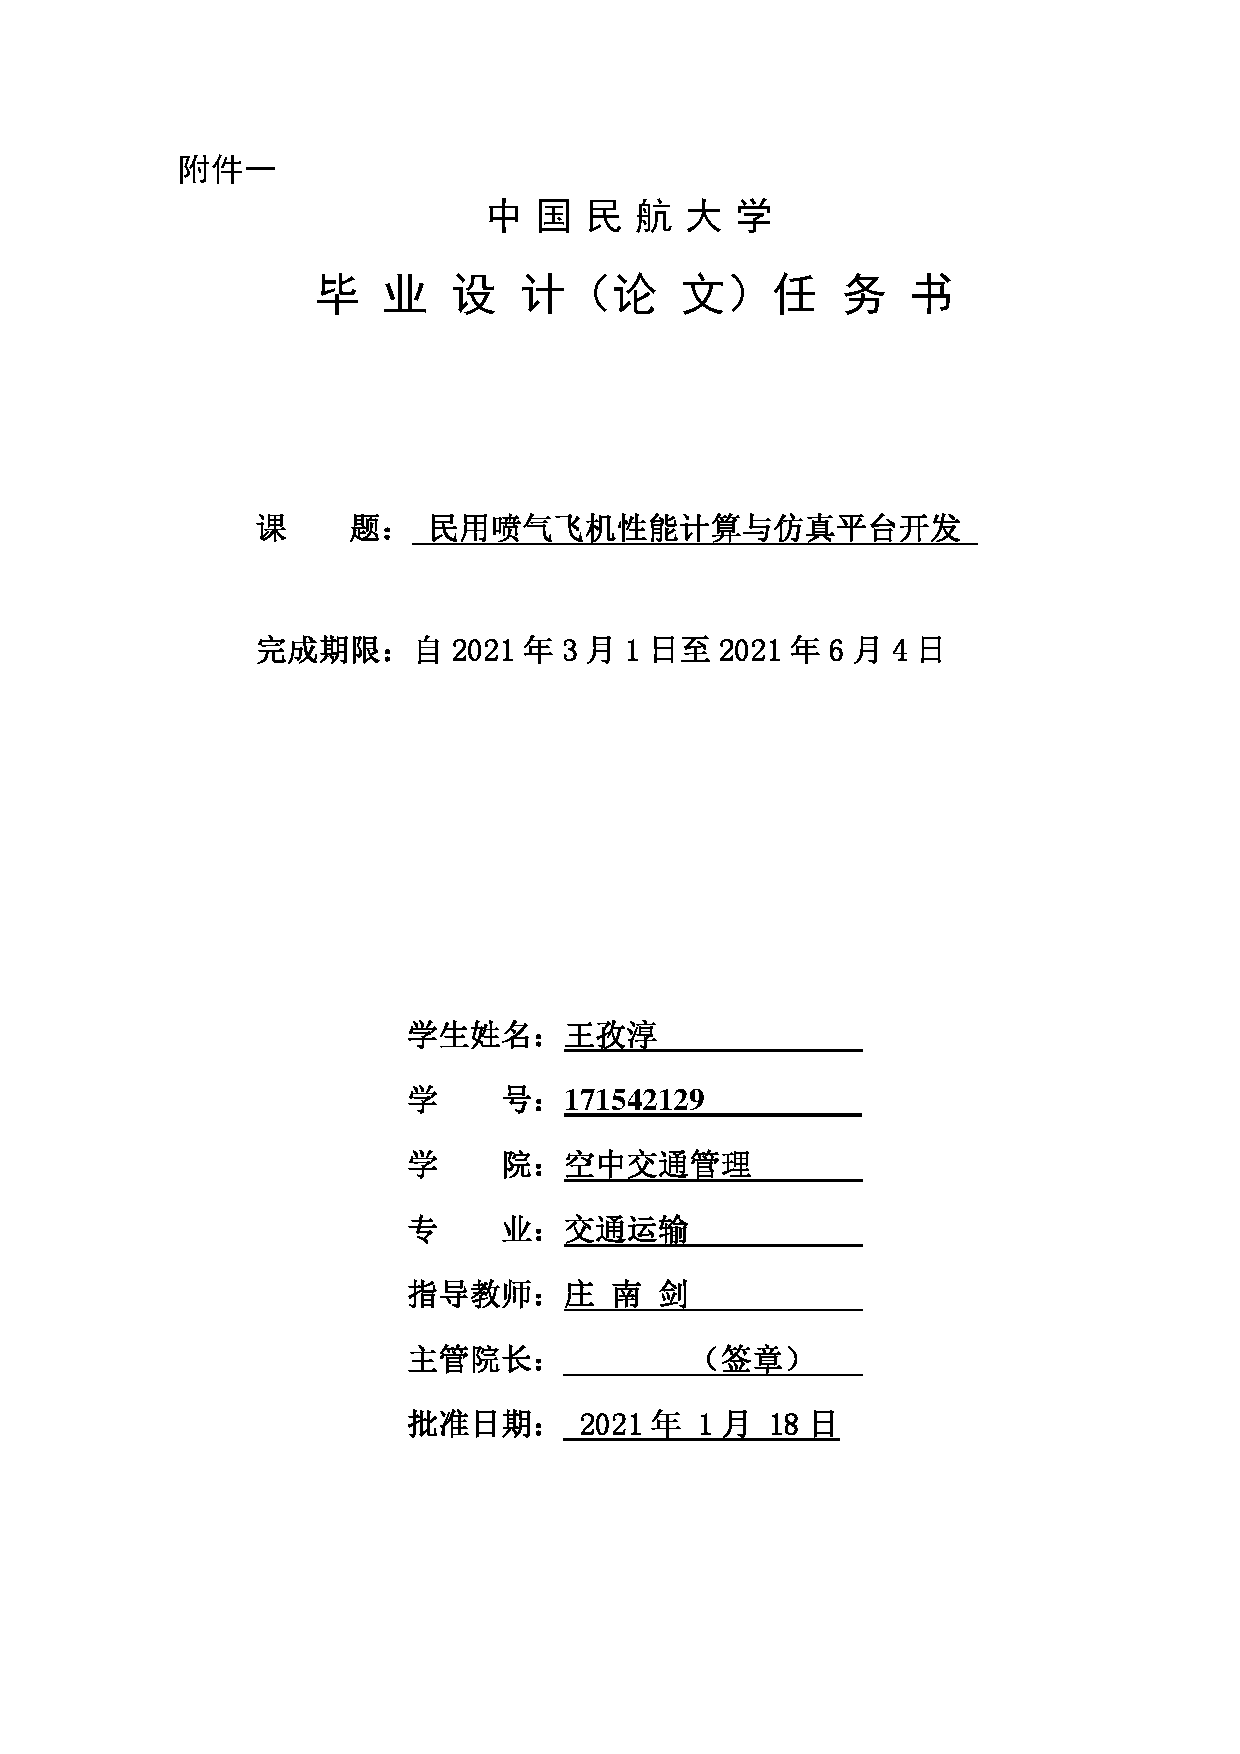
\includepdf[pages=-]{amend.pdf}

\end{document}
